%%%%%%%%%%%%%%%%%%%%%%%%%%%%%%%%%%%%%%%%%%%%%%%%%%%%%%%%%%%%
\documentclass[a4paper,english]{report}    % list options between brackets

\RequirePackage{color}
\RequirePackage{float}
\RequirePackage{amsfonts}
\RequirePackage{amsmath}
\RequirePackage{alltt}
\RequirePackage{ae}
\RequirePackage{times}
\RequirePackage{fancyhdr}
\RequirePackage{graphicx} 
\RequirePackage{makeidx}  

\RequirePackage{hyperref}

\UseRawInputEncoding

\hypersetup{
    bookmarks=true,         % show bookmarks bar?
    unicode=false,          % non-Latin characters in Acrobat�s bookmarks
    pdftoolbar=true,        % show Acrobat�s toolbar?
    pdfmenubar=true,        % show Acrobat�s menu?
    pdffitwindow=false,     % window fit to page when opened
    pdfstartview={Fit},    % fits the width of the page to the window
    pdftitle={Elmer non-GUI Tutorials},    % title
    pdfauthor={CSC - IT Center for Science},     % author
%    pdfsubject={Subject},   % subject of the document
%    pdfcreator={Creator},   % creator of the document
%    pdfproducer={Producer}, % producer of the document
%    pdfkeywords={keywords}, % list of keywords
    pageanchor=true,
    hyperindex=true,
    pdfnewwindow=true,      % links in new window
    colorlinks=true,       % false: boxed links; true: colored links
    linkcolor=black,          % color of internal links
    citecolor=black,        % color of links to bibliography
    filecolor=black,      % color of file links
    urlcolor=black           % color of external links
}
 
\makeindex             
  
%%%%%%%%%%%%%%%%%%%%%%%%%%%%%%%%%%%%%%%%%%%%%%%%%%%%%%%%%%%%

% Use these to make the printable area bigger
% Also have the option 'ownsize' active in the documentclass
\setlength{\hoffset}{-15mm}
\setlength{\voffset}{-10mm}
\addtolength{\textwidth}{30mm}
\addtolength{\textheight}{20mm}
%\addtolength{\headwidth}{30mm}


% Command file syntax stuff
\definecolor{SifCol}{rgb}{0.5,0.5,0.5}
%\definecolor{SifCol}{rgb}{1,1,1}

% Index for keywords
\newcommand{\sifitem}[2]{\item[\tt{#1}]\index{#1}\hspace{1mm}{\color{SifCol}\hspace{1mm}\tt{#2}}\newline} 
%item with two fields but no text
\newcommand{\sifitemnt}[2]{\item[\tt{#1}]\index{#1}\hspace{1mm}{\color{SifCol}\hspace{1mm}\tt{#2}}} 


\newcommand{\sifbegin}{\begin{description}}
\newcommand{\sifend}{\end{description}}
\newcommand{\modinfo}[2]{{\bf{#1}}: {#2}\newline}

\newcommand{\ttbegin}{\begin{alltt}}
\newcommand{\ttend}{\end{alltt}}
\newcommand{\ttitem}[1]{\item[\tt{#1}]\mbox{}\\}
\newcommand{\keno}{$\backslash$}


\newcommand{\Sf}[1]{\textsf{#1}}
\newcommand{\Bf}[1]{{\sffamily\bfseries}}

\newcommand{\URL}[1]{\texttt{#1}}

% Some new commands...
\def\xwin{X Window System}
\def\xbr{Xbrowse}
\def\prag{\Tt{\#pragma}}

\newcommand{\inxgra}[2]{{\centerline{\includegraphics[width=#1]{#2}}}}
\newcommand{\inygra}[2]{{\centerline{\includegraphics[height=#1]{#2}}}}
\newcommand{\incgra}[2]{{\centerline{\includegraphics[height=#1]{#2}}}}

\providecommand{\ftn}{Fort\-ran~90}
\providecommand{\Idx}[1]{{#1}\index{#1}}


%%%%%%%%%%%%%%%% Math definitions for Elmer Solver Manuals %%%%%%%%%%%%%%%%%
\newcommand{\Bfm}[1]{\mbox{\boldmath{${#1}$}}}

\newcommand{\tensorspace}[1]{\boldsymbol{#1}}         % Sets of tensors are bold italic
\newcommand{\tensor}[1]{\boldsymbol{#1}}              % Tensors are bold italic
\newcommand{\point}[1]{\mathbf{#1}}                   % Points are bold upright
\newcommand{\pointf}[1]{\mathbf{#1}}                  % Point-valued functions are bold upright
\newcommand{\pointfm}[1]{\mbox{\boldmath{${#1}$}}}    % Point-valued functions for math symbols

\DeclareMathOperator{\grad}{\mathbf{grad}}            % The spatial gradient operator
\newcommand{\Grad}{\mbox{\boldmath{${\nabla}$}}}      % gradient with respect to the points of the reference configuration
\DeclareMathOperator{\curl}{\mathbf{curl}}            % The spatial curl operator
\DeclareMathOperator{\Curl}{\mathbf{Curl}}            % curl with respect to the points of the reference configuration
\DeclareMathOperator{\rot}{\mathbf{rot}}              % rot operator defined for scalars
\DeclareMathOperator{\divs}{\mathrm{div}}             % scalar-valued divergence
\DeclareMathOperator{\divvec}{\mathbf{div}}           % vector-valued divergence
\DeclareMathOperator{\Divvec}{\mathbf{Div}}           % vector-valued divergence w. r. t. the points of the reference configuration
\newcommand{\Div}{\nabla\cdot}                        

%\newcommand{\Vec}[1]{\vec{#1}}
%\newcommand{\Vec}[1]{\mathify{\mathbf{#1}}}

%\newcommand{\Matr}[1]{\mbox{${#1}$}}                  % Matrices are just italic to differentiate between true tensors and matrices
\newcommand{\Matr}[1]{{#1}}                     % Matrices
\newcommand{\Der}[2]{\frac{\partial{#1}}{\partial{#2}}}
\newcommand{\Secder}[2]{\frac{\partial^2{#1}}{\partial{#2}^2}}
\newcommand{\Inv}[1] {\frac{1}{#1}}


% Make the headings fancier
\pagestyle{fancy}

\lhead[\normalfont\small\bf\thepage]{\normalfont\small\slshape\rightmark}
\rhead[\small\slshape\lefthead]{\normalfont\small\bf \thepage}
%\setlength{\headrulewidth}{0.4pt}
%\renewcommand{\chaptermark}[1]{\markright{\bf \chaptername \ \thechapter.\ #1}{}}
%\renewcommand{\chaptermark}[1]{\markright{\bf \thechapter.\ #1}{}}
\renewcommand{\sectionmark}[1]{}
\renewcommand{\subsectionmark}[1]{}
\cfoot{}

% This sets the Elmer version in the documentation
%\newcommand{\elmerversion}{6.0}



% This sets the Elmer version in the documentation
\newcommand{\elmerversion}{8.4}


%%%%%%%%%%%%%%%%%%%%%%%%%%%%%%%%%%%%%%%%%%%%%%%%%%%%%%%%%%%%

\title{\Huge{\bf Elmer non-GUI Tutorials}}
\author{CSC -- IT Center for Science}
\date{\today}

%%%%%%%%%%%%%%%%%%%%%%%%%%%%%%%%%%%%%%%%%%%%%%%%%%%%%%%%%%%%

\begin{document}
\vbox{
  \centering
  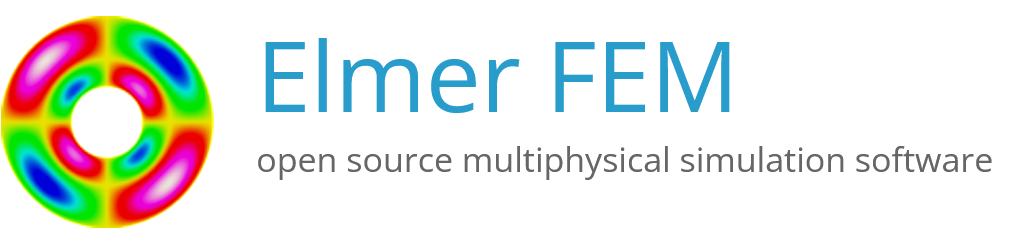
\includegraphics[width=0.9\textwidth]{../elmerlogo}
  \maketitle
}

\chapter*{Get Started with Elmer}

\section*{About this document}

This document, Get Started with Elmer, is intended to help anyone who has just downloaded Elmer and would like some help getting started.\\

The first three chapters are provided specifically for Windows users, with detailed instructions to download, install, and start using Elmer.  The instructions have been tested on Windows 10.\\

The rest of the chapters in this document generally apply to all users, running Windows, Linux, and MacOS.\\

Topics discussed include:

\begin{itemize}
  \item Paraview and ElmerVTK for post processing Elmer results
  \item Using Elmer, where to find test cases, tutorials, the Elmer user forum, and youtube video
  \item Parallel operation of Elmer
  \item External tools with Elmer, such as Gmsh and Salome, providing examples of creating multiple bodies
  \item Elmerfem Wiki, a copy of the old wiki
  \item Installing the Elmer Virtual Machine
  \item Installing Elmer in Linux
\end{itemize}


The present manual corresponds to Elmer software version~\elmerversion{}.\\

Latest documentations and program versions of Elmer are available (or links are provided) at \url{http://www.csc.fi/elmer}. \\

\section*{Copyright information}

This document is licensed under the Creative Commons Attribution-NonCommerical 3.0 License.  To view a copy of this license, visit \url{http://creativecommons.org/licenses/by-nc/3.0/}.\\

Initially this document, Get Started with Elmer, has been written by Rich Bayless.  External contributions are welcome.





%%%%%%%%%%%%%%%%%%%%%%%%%%%%%%%%%%%%%%%%%%%%%%%%%%%%%%%%%%%%

%\pagenumbering{roman}
\pagestyle{empty}

% Table of contents:
\setcounter{secnumdepth}{2}
\setcounter{tocdepth}{1}  % set this to 1 in the final version

\phantomsection
\addcontentsline{toc}{part}{Table of Contents}
\tableofcontents

%%%%%%%%%%%%%%%%%%%%%%%%%%%%%%%%%%%%%%%%%%%%%%%%%%%%%%%%%%%%

\newpage

\renewcommand{\chaptername}{Tutorial}

% change the plain style used for chapter pages
\fancypagestyle{plain}{
\lhead{}
\rhead{}
\rfoot{
\includegraphics[width=18mm]{by-nc}}
\lfoot{\footnotesize{CSC -- IT Center for Science}}
\chead{}
%\cfoot{\bfseries \thepage}
\cfoot{}
\renewcommand{\headrulewidth}{0.0pt}
}

% and the fancy style used elsewhere
\pagestyle{fancy}
\rhead{\bfseries \thepage}
\lhead{\bfseries \rightmark}
\rfoot{
\includegraphics[width=18mm]{by-nc}}
\lfoot{\footnotesize{CSC -- IT Center for Science}}
\chead{}
\cfoot{}
\renewcommand{\headrulewidth}{0.4pt}
\renewcommand{\footrulewidth}{0.4pt}


%%%%%%%%%%%%%%%%%%%%%%%%%%%%%%%%%%%%%%%%%%%%%%%%%%%%%%%%%%%%
\clearpage
%\pagenumbering{arabic}

 
%\part{non-GUI Problems}

\graphicspath{{./}{ElasticEigenValues/}}
\chapter{Eigenvalue analysis of an elastic beam}

\modinfo{Directory}{ElasticEigenValues}
\modinfo{Solvers}{\Idx{StressSolve}, \Idx{EigenSolve}}
\modinfo{Tools}{\Idx{ElmerGrid},Editor}
\modinfo{Dimensions}{3D, Steady-state}

\subsection*{Case definition}

A homogenous, elastic silicon beam of dimensions 1 m length, 0.1 m height and 0.2 m width
is supported on its both ends (boundaries 1 and 2). 
A beam has the density 2330 kg/m$^{3}$, Poisson ratio 0.3 and Young's modulus 10$^{11}$ N/m$^{2}$. The problem is to calculate the eigenvalues of the beam. Mathematically the equation to be solved is
\begin{displaymath}
-\rho \omega^{2}\phi = \nabla\cdot\tau(\phi)
\end{displaymath}
where $\rho$ is the density, $\omega$$^{2}$ is the eigenvalue, $\omega$ is the angular frequency, $\phi$ is the corresponding vibration mode and $\tau$ is the stress tensor.

\begin{figure}[h]
\centering
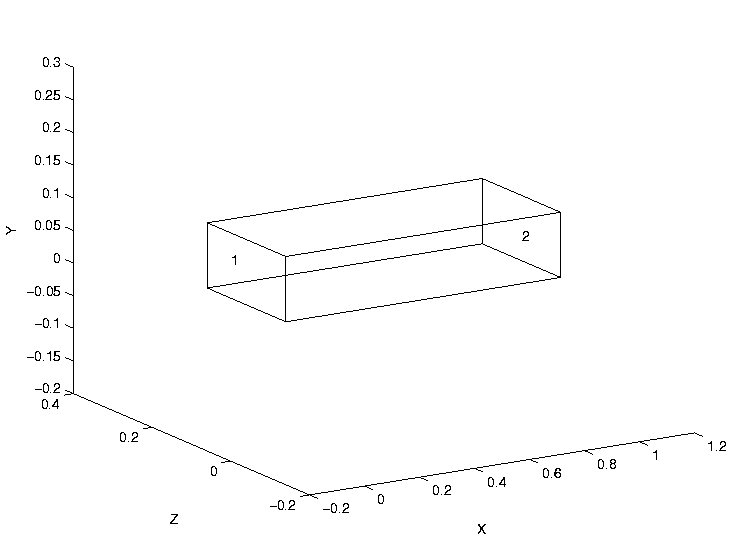
\includegraphics[height=80mm]{palkki}
\caption{Beam.}\label{fg:palkki}
\end{figure}




\subsection*{Solution procedure}

The mesh has been created by using Gambit software and it consists of 2500 elements. The mesh can be converted to Elmer format with ElmerGrid with the command

\ttbegin
ElmerGrid 7 2 mesh.FDNEUT
\ttend

\begin{flushleft}
This command creates the directory which contains the Elmer mesh files.


\ttbegin
Header
  Mesh DB "." "mesh"
  Include Path ""
  Results Directory ""
End
\ttend

A steady-state three-dimensional analysis is defined in the simulation section.

\ttbegin
Simulation
  Coordinate System = "Cartesian 3D"
  Coordinate Mapping(3) = 1 2 3
  Simulation Type = "Steady State"
  Steady State Max Iterations = 1
  Solver Input File = "eigen_values.sif"
  Output File = "eigen_values.dat"
  Post File = "eigen_values.vtu"
End
\ttend 

The geometry of the problem is simple and it includes only one body and material. 

\ttbegin
Body 1
  Equation = 1
  Material = 1
End

Material 1
  Youngs Modulus = 100e9
  Poisson Ratio = 0.3
  Density = 2330
End
\ttend

The problem is solved according to linear elastic theory and due to that stress analysis is set to true.

\ttbegin
Equation 1
  Stress Analysis = True
End
\ttend

In the solver section {\tt Stress Analysis} is selected. In addition, the value of the keyword 
{\tt Eigen Analysis} has to be set to true. The keyword {\tt Eigen System Values} defines the number of the computed eigenvalues. The problem also is possible to solve with iterative solver but we have used direct solver in this example.

\ttbegin
Solver 1
  Equation = "Stress Analysis"
  Eigen Analysis = Logical True
  Eigen System Values = Integer 5
  Linear System Solver = "direct"

  Variable = "Displacement"
  Variable Dofs = 3
  Linear System Iterative Method = "BiCGStab"
  Linear System Max Iterations = 1000
  Linear System Convergence Tolerance = 1.0e-08
  Linear System Abort Not Converged = True
  Linear System Preconditioning = "ILU0"
  Linear System Residual Output = 1
  Steady State Convergence Tolerance = 1.0e-05
  Nonlinear System Convergence Tolerance = 1.0e-05
  Nonlinear System Max Iterations = 1
  Nonlinear System Newton After Iterations = 3
  Nonlinear System Newton After Tolerance = 1.0e-02
  Nonlinear System Relaxation Factor = 1
  Linear System Precondition Recompute = 1
End
\ttend

The beam is supported on its both ends and therefore displacements are set to zero in all directions.

\ttbegin  
Boundary Condition 1
  Target Boundaries(1) = 1
  Displacement 1 = 0
  Displacement 2 = 0
  Displacement 3 = 0  
End

Boundary Condition 2
  Target Boundaries(1) = 2
  Displacement 1 = 0
  Displacement 2 = 0
  Displacement 3 = 0  
End
\ttend  

After that, the problem is ready to solve.
\linebreak[4]

\begin{bf}
An anisotropic model
\end{bf}
\linebreak[2]

The same problem can also be solved as an anisotropic problem
which causes a couple of changes in the sif-file.
First, it is reasonable to rename the files in the simulation section

\ttbegin
Solver Input File = "eigen_values_aniso.sif"
Output File = "eigen_values_aniso.dat"
Post File = "eigen_values_aniso.vtu"
\ttend

For anisotropic material Young's modulus has to be redefined as a matrix. 
In this case the matrix is defined as follows

\ttbegin
Youngs Modulus
Size 6 6
    Real  200e9  60e9   60e9   0     0     0      
          60e9   200e9  200e9  0     0     0      
          60e9   60e9   200e9  0     0     0      
          0      0      0      80e9  0     0      
          0      0      0      0     80e9  0      
          0      0      0      0     0     80e9   
    End
\ttend

No more changes are needed in the sif-file.

\end{flushleft}
\subsection*{Results}
Both the eigenvalues of the isotropic and the eigenvalues of the anisotropic model are shown below in Elmer outputs. Figure \ref{fig:eig12345} presents the computed eigenvectors of the beam with the isotropic model. The formula $\omega$ = 2$\pi$$f$ have been used in calculating frequencies ($f$)
(Table \ref{tb:freq}).
According to the results the anisotropic model yielded greater eigenvalues with
these values of Young's modulus.  


\ttbegin
EigenSolve: Computed Eigen Values:
EigenSolve: --------------------------------
EigenSolve:            1        (16737546.4275755,0.00000000000000D+000)
EigenSolve:            2        (48175589.4544061,0.00000000000000D+000)
EigenSolve:            3        (99674749.0526558,0.00000000000000D+000)
EigenSolve:            4        (110392974.959463,0.00000000000000D+000)
EigenSolve:            5        (253947166.278411,0.00000000000000D+000)

\ttend
\begin{center}
Isotropic model.
\end{center}
\ttbegin
EigenSolve: Computed Eigen Values:
EigenSolve: --------------------------------
EigenSolve:            1        (29608629.8775828,0.00000000000000D+000)
EigenSolve:            2        (88782964.0905879,0.00000000000000D+000)
EigenSolve:            3        (198583949.415515,0.00000000000000D+000)
EigenSolve:            4        (205085884.544046,0.00000000000000D+000)
EigenSolve:            5        (480903841.387323,0.00000000000000D+000)
\ttend
\begin{center}
Anisotropic model.
\end{center}
\begin{table}[h]
\caption{Computed frequencies.}
\label{tb:freq}
\begin{center}
\begin{tabular}{lll} \hline
step  & isotropic & anisotropic\\ \hline
1 & 651.127 Hz  & 866.023 Hz\\
2 & 1104.673 Hz & 1499.633 Hz\\
3 & 1588.959 Hz & 2242.809 Hz\\
4 & 1672.210 Hz & 2279.229 Hz      \\
5 & 2536.249 Hz & 3490.191 Hz    \\ \hline
\end{tabular}
\end{center}
\end{table}


\begin{figure}[h!]
\begin{center}
  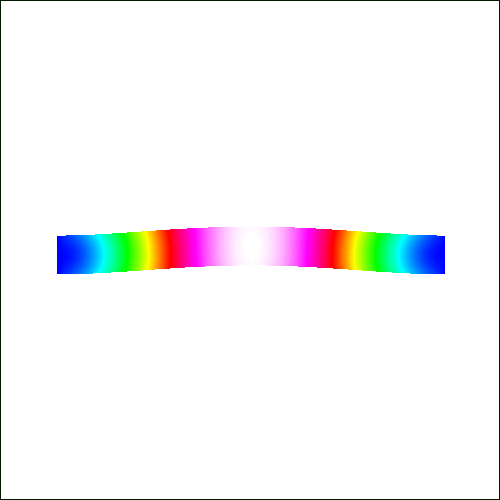
\includegraphics[width=0.4\textwidth,angle=0]{eig1}
  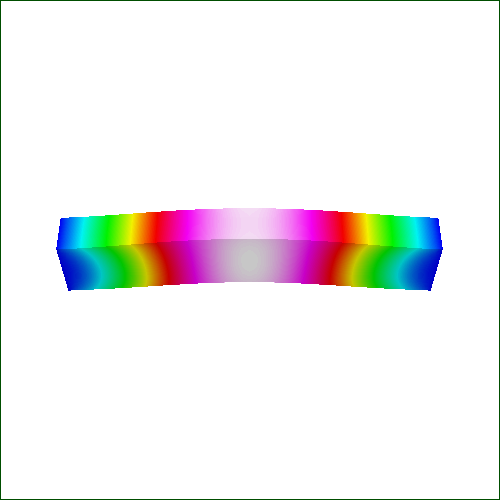
\includegraphics[width=0.4\textwidth,angle=0]{eig2}
  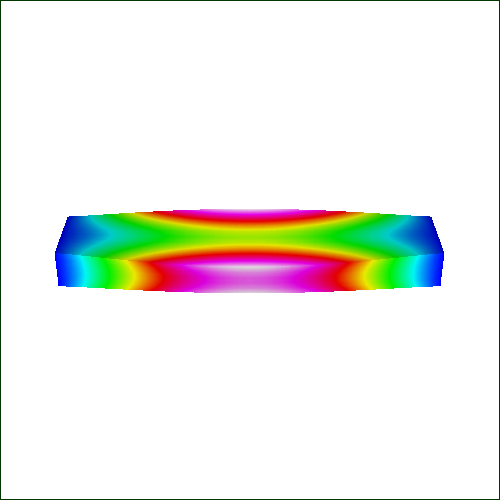
\includegraphics[width=0.4\textwidth,angle=0]{eig3}
  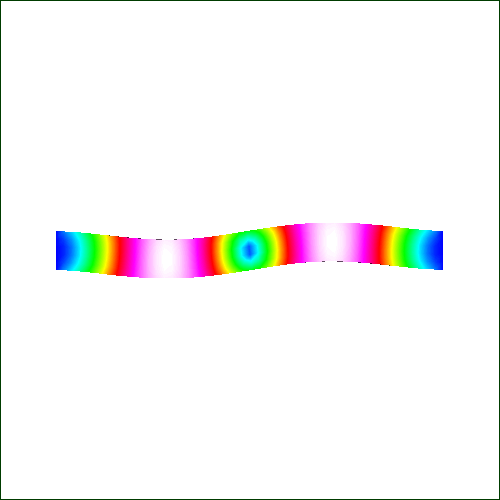
\includegraphics[width=0.4\textwidth,angle=0]{eig4}
  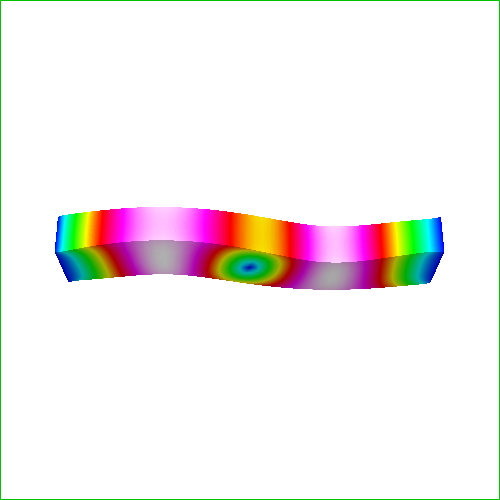
\includegraphics[width=0.4\textwidth,angle=0]{eig5}
  \caption{Eigenvectors}
  \label{fig:eig12345}
\end{center}
\end{figure}

\vfill


\graphicspath{{./}{FlowResistance/}}
\chapter{Flow through a hole -- determining the acoustic impedance} 

\modinfo{Directory}{FlowResistance}
\modinfo{Solvers}{\Idx{FlowSolve}}
\modinfo{Tools}{\Idx{ElmerGrid}, editor}
\modinfo{Dimensions}{3D, Steady-state}

\noindent
Note: This test case is available as consistency tests 
\texttt{FlowResNoslip} and \texttt{FlowResSlip}. This may be outdated
in parts. For example, it is not necessary to use any special unit system,
and also the computation of forces is now more accurate.

\subsection*{Case definition}

The problem at hand consists of finding the resistance that a fluid
faces as it is forced to flow through a hole. The flow resistance is
stated by the ratio of pressure drop over the hole and the input
velocity. In micro-system modeling, the hole resistance is often needed
to analyse the gas damping effect in perforated structures. Here, the
contribution of the holes is homogenized over the perforated structure
based on a single hole resistance. For homogenization in Elmer, the
specific \Idx{acoustic impedance} is used to represent the flow
resistance. Specific acoustic impedance $z_h$ is defined as
\begin{equation}
z_h = \frac{p}{v} = \frac{F}{vA_h},
\end{equation}
where $F$ is the net force due to gas on the moving surface, $v$ is
the velocity of the gas on the same surface, and $A_h$ is the area of
the moving surface. The calculation is best performed in a unit cell
of the geometry.

In order to the homogenization to be possible, the dependence of input
velocity and the net force should be linear. Further, there should not
be a phase change between these two quantities. These conditions are
satisfied when the flow is incompressible.  In a linear case, the
fluid flow can be treated with the linear form of Navier-Stokes
equations called the \Idx{Stokes equation}
\begin{equation}
\rho\frac{\partial \vec{u}}{\partial t}
-\nabla\cdot(2\eta\overline{\overline{\varepsilon}}) +\nabla p =
\rho \vec{f},
\end{equation}
where $\vec{u}$ is the unknown velocity field, $p$ is the pressure,
$\eta$ is the viscosity of the fluid, $\rho\vec{f}$ is a body force
and $\overline{\overline{\varepsilon}}$ is the linearised strain
tensor. Note, that the stationary version of the above equation can be
used in homogenization calculations.

The condition for Stokes equation to apply is that the Reynolds number
$Re$ of the problem should be small
\begin{equation}
Re = \frac{\rho UL}{\eta},
\end{equation}
where $\rho$ is density of the fluid and $U$ and $L$ are,
respectively, the velocity and length scales of the problem.

The issue of compressibility is more difficult to answer. A classical
condition for the compressibility is that the Mach number $Ma$ of the
problem should be small
\begin{equation}
Ma = \frac{U}{a} < 0.3,
\end{equation}
where $a$ is the speed of sound in the gas in operating conditions and
the value~0.3 is often stated limit for a small Mach number (actually,
the condition is that $Ma^2$ has to be small).  Also the frequency and
amplitude of the oscillations of the system have an effect on the
validity of the linearity and incompressibility assumptions, since
they affect the velocity scale of the problem.

However, also other factors have an effect on the compressibility of
the gas. In micro-systems, the viscous effects on pressure, or even
temperature changes, can affect the density of the gas. A
condition for viscous pressure changes is that $Ma^2/Re$ has to be
small, and for temperature, in addition, that the Prandtl number $Pr$
may not be too large
\begin{equation}
Pr = \frac{\eta c_p}{k},
\end{equation}
where $c_p$ is the heat capacity ({\em ie.} specific heat) in constant
pressure and $k$ is the thermal conductivity.

The conditions listed here for the flow to be approximately
incompressible are only an overview and the validity of
incompressibility assumption should be considered in each case
separately. In micro-systems, refer for example to the article
M.~Gad-el-Hak, J.~Fluids Eng., 121, 5--33, 1999. Additionally, it is
advisable to perform numerical checks on the issue.

One final point on the applicability of the Stokes (or Navier-Stokes)
equations is the effect of gas rarefaction. If the dimensions of the
problem are very small the continuity assumption may not be valid
anymore. The importance of the gas rarefaction effects are given by
the Knudsen number $Kn$
\begin{equation}
Kn = \frac{{\cal L}}{L},
\end{equation}
where ${\cal L}$ is the mean free path of the gas molecules. The mean
free path depends inversely on ambient pressure, which has to take
into account in stating the Knudsen number. For Knudsen numbers close
to and less than~1, slip boundary conditions should be used.

To summarize, the motivation of this tutorial is to perform a linear
incompressible simulation of fluid flowing through a hole. The wake
for the flow is a constant velocity boundary condition for a boundary
before the hole. On the same boundary, the force caused by the fluid
is recorded. These two quantities can then be used to determine the
specific acoustic impedance of a single hole. The constant velocity
boundary condition may be interpreted as describing a moving wall with
small displacement. In this particular tutorial, a symmetrical
quadrant of a square-shaped hole is used.



\subsection*{Solution procedure}

The solution for the problem is found by solving iteratively the
Stokes equation. Nonlinear iterations are not needed, since the
problem is linear.

The computational mesh should include enough free space after the hole
so that any artificial effects due to the boundaries of the mesh are
avoided. In this tutorial, the geometry is created and meshed using
the ElmerGrid program by the command
{\tt
elmergrid 1 2 hole.grd}. 
The default mesh consists of about 12000 nodes and 10500 eight-noded
hexahedrons.

The header section of solver input file includes only the location of
the mesh files.
\ttbegin
Header
  Mesh DB "." "hole"
End
\ttend

In the simulation section, a steady-state three-dimensional analysis
is defined.
\ttbegin
Simulation
  Coordinate System = Cartesian 3D
  Simulation Type = Steady State
  Steady State Max Iterations = 1
  Output File = "flow.result"
  Post File = "flow.vtu"
End
\ttend

The geometry contains only one body and no body forces or initial
conditions are present. The body section reads thus as follows.
\ttbegin
Body 1
  Equation = 1
  Material = 1
End
\ttend

For solving the flow patterns the Navier-Stokes solver is used but the
nonlinearity through convection is switched off in the equation block.
Also, solvers for the fluidic force and saving data are enabled.
\ttbegin
Equation 1
  Active Solvers(3) = Integer 1 2 3
  NS Convect = False
End
\ttend

Just a single iteration of the Navier-Stokes solver is needed, since
the equation is linear. This can be verified by switching the number
of nonlinear iterations to a value more than one, and observing the
change in solution between iteration steps.
\ttbegin
Solver 1
   Equation = Navier-Stokes
   Variable = Flow Solution
   Variable DOFs = 3
   Linear System Solver = Iterative
   Linear System Iterative Method = BiCGStab
   Linear System Preconditioning = ILU0
   Linear System Max Iterations = 200
   Linear System Convergence Tolerance = 1.0e-08
   Stabilize = True
   Nonlinear System Convergence Tolerance = 1.0e-05
   Nonlinear System Max Iterations = 1
   Nonlinear System Newton After Iterations = 3
   Nonlinear System Newton After Tolerance = 1.0e-08
   Nonlinear System Relaxation Factor = 1.0
   Steady State Convergence Tolerance = 1.0e-05
End
\ttend

The fluidic force solver needs to be run only once, after the flow
solution is finished. With the keyword {\tt Calculate Viscous Force} it
is possible to define whether the viscous forces of the fluid are
included in the force or not. If this is set to false, only the
pressure integral is calculated.
\ttbegin
Solver 2
  Exec Solver = After All
  Equation = Fluidic Force
  Procedure  ="FluidicForce" "ForceCompute"
  Calculate Viscous Force = True
End
\ttend

The final solver is used to save data from the analysis. With the
following definitions, the input velocity and the net force on the
input boundary as well as the area of the boundary are written into a
file called {\tt flowdata.dat}.
\ttbegin
Solver 3
  Exec Solver = After All
  Equation = SaveScalars
  Procedure = "\Idx{SaveData}" "SaveScalars"
  Filename = "flowdata.dat"
  Save Variable 1 = Velocity 3
  Save Coordinates(1,2) = 0.0 0.0
End
\ttend

The fluid is defined to be air. Note the Elmer \Idx{MEMS} units used.
\ttbegin
Material 1
  Name = Air
  Density = 1.293e-12
  Viscosity = 1.67e-5
End
\ttend

Finally, the boundary conditions. BC~1 defines the input boundary,
where also the fluidic force is calculated. BCs~2 and~4 define the
symmetry boundaries, BC~3 defines the no-slip conditions for the
walls, and BC~5 defines an open boundary.
\ttbegin
Boundary Condition 1
  Target Boundaries = 4
   Velocity 1 = 0.0
   Velocity 2 = 0.0
   Velocity 3 = 1.0e3
   Calculate Fluidic Force = True
End

Boundary Condition 2
  Target Boundaries(2) = 8 10
   Velocity 2 = 0.0
End

Boundary Condition 3
  Target Boundaries(4) = 1 2 3 7
   Velocity 1 = 0.0
   Velocity 2 = 0.0
   Velocity 3 = 0.0
End

Boundary Condition 4
  Target Boundaries(2) = 6 9
   Velocity 1 = 0.0
End

Boundary Condition 5
  Target Boundaries = 5
  Pressure = 0.0
End
\ttend

\subsection*{Slip boundary conditions}

The same simulation can also be performed using slip boundary
conditions. These are appropriate, as stated in the introduction, when the
Knudsen number is between $10^{-3}$ and 1. The slip boundary condition
implemented in Elmer is of first order 
\begin{equation}
S\cdot \vec{u} = \overline{\overline{\sigma}}\cdot\vec{n},
\end{equation}
where $S$ is a vector containing the slip coefficients $s_i$ for each
velocity component, $\mu$ is the viscosity, and
$\overline{\overline{\sigma}}$ is the stress tensor. For Newtonian
fluids and for tangential directions of the boundary this gives
\begin{equation}
s_i u_i = \mu\frac{\partial u_i}{\partial n},
\end{equation}
where $s_i$ and $u_i$ refer to the same tangential component of the
slip coefficient and the flow velocity.

The value of the slip coefficient is related to the mean free path of
the gas molecules $\lambda$. For example, Maxwell's first order slip
boundary condition may be used (as in {\em e.g.} A.~Beskok, {\em
Num. Heat Transfer,} B, 40, 451--471, 2001):
\begin{equation}
u_i = \frac{2-\sigma_v}{\sigma_v}\lambda 
\frac{\partial u_i}{\partial n},
\end{equation}
where $\sigma_v$ is the tangential momentum accommodation coefficient,
which models the momentum exchange of gas molecules and the
surface. The accommodation coefficient is dependent on the gas and on
the surface, and recent measurements give a result of $\sigma_v\simeq
0.80$ for various monoatomic gases such as Argon in contact with
prime Silicon crystal. 

The slip coefficient of Elmer can finally be written as
\begin{equation}
s_i = \frac{\mu}{\lambda}\frac{\sigma_v}{2-\sigma_v}.
\end{equation}
The mean free path is defined as
\begin{equation}
\lambda = \frac{\mu}{\rho}\sqrt{\frac{\pi M}{2RT}}_,
\end{equation}
where $\rho$ is density, $M$ is the molar mass, $T$ is the
temperature, and $R=8.3145$~J/mol~K is the molar gas constant.

In the Elmer analysis, only a few changes in the sif-file are needed
to make the slip conditions active. The flow force boundary conditions
have to be turned on and the numerical value of the slip coefficient
has to be defined on each boundary (here $s=$2e-4 is used for
air). Further below is a list of the Boundary Condition blocks. Note
that there are more BCs than in the no-slip simulation, since a
separate condition is needed for surfaces oriented differently in
space.

Generally, a normal-tangential orientation scheme for the boundary
conditions are needed, since the surfaces are not necessarily having a
normal vector pointing in one of the coordinate directions. This would
be done for each such boundary by the line
\ttbegin
  Normal-Tangential Velocity = True
\ttend
after which the Velocity component~1 points to the normal direction
and the other components to the tangential directions.

\ttbegin
! Definitions for slip boundary conditions:
Boundary Condition 1
  Target Boundaries = 4
   Flow Force BC = True
   Slip Coefficient 1 = 2e-4
   Slip Coefficient 2 = 2e-4
   Velocity 3 = 2.0e3
   Calculate Fluidic Force = True
End

Boundary Condition 2
  Target Boundaries(2) = 8 10
   Velocity 2 = 0.0
End

Boundary Condition 3
  Target Boundaries(2) = 2 3
   Flow Force BC = True
   Velocity 3 = 0.0
   Slip Coefficient 1 = 2e-4
   Slip Coefficient 2 = 2e-4
End

Boundary Condition 4
  Target Boundaries(2) = 6 9
   Velocity 1 = 0.0
End

Boundary Condition 5
  Target Boundaries = 5
  Pressure = 0.0
End

Boundary Condition 6
  Target Boundaries = 1
   Flow Force BC = True
   Velocity 1 = 0.0
   Slip Coefficient 2 = 2e-4
   Slip Coefficient 3 = 2e-4
End

Boundary Condition 7
  Target Boundaries = 7
   Flow Force BC = True
   Velocity 2 = 0.0
   Slip Coefficient 1 = 2e-4
   Slip Coefficient 3 = 2e-4
End
\ttend

\subsection*{Results}

The computation takes about 200~cpu seconds on an AlphaServer with
1~GHz central processor when trilinear elements are used (historical results).
The results
for two different input velocities taken from the file {\mbox{\tt
flowdata.dat}} are summarised in Table~\ref{tab:imped_res}. Also the
specific acoustic impedance $z_h$ is calculated in the table. The
results of slip and no-slip simulations are also compared.  Note that
for the force, only the component perpendicular to the surface should
be used since the other components cancel out due to symmetry. The
values in the table are again given in Elmer MEMS units (these units
are numerically favourable in small dimensions and were used historically
in MEMS projects).
\begin{table}[htb]
\caption{Results of flow simulations for two input velocities}
\label{tab:imped_res}
\begin{center}
\begin{tabular}{cccc} \hline
$v$ & \ \ slip model\ \  & $F_z$ & $z_h$ \\ \hline 
$1.0\cdot 10^3$   & no-slip  & 36.13  &  $1.45\cdot10^{-3}$ \\
$2.0\cdot 10^3$   & no-slip  & 72.25  &  $1.45\cdot10^{-3}$ \\ \hline
$1.0\cdot 10^3$   & slip     & 29.30  &  $1.17\cdot10^{-3}$ \\
$2.0\cdot 10^3$   & slip     & 58.60  &  $1.17\cdot10^{-3}$ \\ \hline
\end{tabular}
\end{center}
\end{table}

The identical values obtained for the spesific acoustic impedance in
Table~\ref{tab:imped_res} prove by no means that the flow in reality
is linear, since this was the assumption and the simulation performed
can and should not reveal any nonlinear behavior. The results
indicate, though, that allowing slip on the boundaries reduces the
resistance that the fluid faces. This example shows that in
micro-systems, as the dimension of the smallest flow channel is in the
range of a micrometer, it is reasonable to use slip boundary
conditions for the velocity.

\begin{figure}[htb]
  \centerline{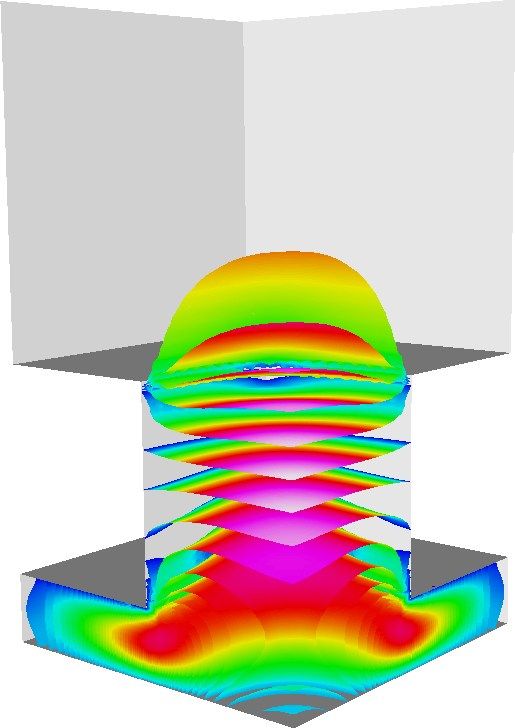
\includegraphics[width=0.40\textwidth]{flow_res}}
  \caption{The linear flow results.} 
  \label{fig:flow_res}
\end{figure}
Finally, a picture of the results obtained with no-slip conditions is
presented. The Fig.~\ref{fig:flow_res} shows a lot of pressure
isosurfaces which are coloured using the absolute value of the
velocity.

Note: it seems that the results with the current code are not
exactly the same. However, we didn't invest where the small discrepancy
might come from. 


\vfill
\mbox{}


\graphicspath{{./}{Electrostatics/}}
\chapter{Electrostatics}

\modinfo{Directory}{Electrostatics}
\modinfo{Solvers}{\Idx{StatElecSolve}, \Idx{ElectricForce}}
\modinfo{Tools}{\Idx{ElmerGrid}, editor}
\modinfo{Dimensions}{3D, Steady-state}

\subsection*{Case definition}

This case presents solving the Poisson equation for electric potential
and calculating appropriate derived quantities, such as
\Idx{capacitance}, based on the result. The geometry studied is a
symmetric quadrant of a plane capacitor having a rectangular hole in
another plate. A setting of this kind can be used to study the effects
of geometrical features on the capacitance and on the electrostatic
force, which both are meaningful quantities for coupled
simulations in {\em e.g.}  microsystems.


\subsection*{Solution procedure}

The mesh is constructed using ElmerGrid with the following command
\ttbegin
ElmerGrid 1 2 elmesh.grd
\ttend
The mesh is extended above the hole to avoid undesired boundary
effects. The geometry is presented in the Figure~\ref{geo_elstat}

\begin{figure}[hbt]
  \centerline{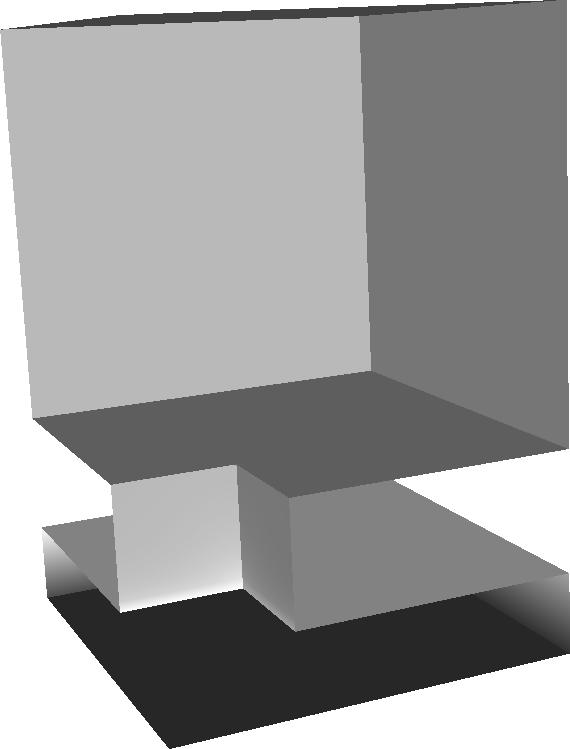
\includegraphics[width=0.32\textwidth]{geo_elstat}}
  \caption{The geometry of problem.} 
  \label{geo_elstat}
\end{figure}

The simulation problem includes a single body, and thus one material
and one equation set, as well as three solvers. The solvers are used
to compute the electric potential and related quantities, to calculate
the electric force, and to save relevant data into a file. This
tutorial is defined in Elmer \Idx{MEMS} units. The sif-file is presented
below.

\ttbegin
Check Keywords Warn

Header
  Mesh DB "." "elmesh"
End
\ttend

Only a single steady state iteration is needed, since the Poisson
equation is linear.
\ttbegin
Simulation
  Coordinate System = Cartesian 3D
  Simulation Type = Steady State
  Steady State Max Iterations = 1
  Output File = "elstatics.result"
  Post File = "elstatics.vtu"
End
\ttend

The permittivity of vacuum has to be defined in the Constants section.
\ttbegin
Constants
  Permittivity Of Vacuum = 8.8542e-12
End

Body 1
  Equation = 1
  Material = 1
End
\ttend

Electric energy density is added into the results in Equation
section. This allows energy density to be visualised.
Here the visualization is done with now obsolete ElmerPost
but you would probably rather use Paraview (or some other software that
can handle VTU files). 
Note also, that calculating electric flux (or the electric
displacement field) is disabled in the Solver~1 block. Further, the
potential difference used in calculating the capacitance of the system
has to be defined in this section. This should be the same as the
boundary conditions define for the capacitance calculation to be
sensible.
\ttbegin
Equation 1
  Active Solvers(2) = 1 2
  Calculate Electric Energy = True  ! (default False)
End

Solver 1
  Equation = Stat Elec Solver
  Variable = Potential
  Variable DOFs = 1
  Procedure = "StatElecSolve" "StatElecSolver"
  Calculate Electric Field = True  ! (default True)
  Calculate Electric Flux = False  ! (default True)
  Potential Difference = 1.0e6
  Linear System Solver = Iterative
  Linear System Iterative Method = BiCGStab
  Linear System Max Iterations = 200
  Linear System Convergence Tolerance = 1.0e-07
  Linear System Preconditioning = ILU1
  Linear System ILUT Tolerance = 1.0e-03
  Nonlinear System Max Iterations = 1
  Nonlinear System Convergence Tolerance = 1.0e-4
  Nonlinear System Newton After Tolerance = 1.0e-3
  Nonlinear System Newton After Iterations = 10
  Nonlinear System Relaxation Factor = 1
  Steady State Convergence Tolerance = 1.0e-4
End
\ttend

The static electric force solver does not need a lot of
information:
\ttbegin
Solver 2
  Equation = Electric Force
  Procedure = "ElectricForce" "StatElecForce"
End
\ttend

Finally, some data is saved in file scalars.dat in working directory.
\ttbegin
Solver 3
  Exec Solver = After All
  Equation = SaveScalars
  Procedure = "\Idx{SaveData}" "SaveScalars"
  Filename = "scalars.dat"
End
\ttend

Only the relative permittivity of the material has to be defined.
\ttbegin
Material 1
  Relative Permittivity = 1
End
\ttend

The boundary conditions include the values of electric potential
(voltage) and indication on which boundary the electric force should
be calculated. On all the other boundaries a natural boundary
condition is used, basically stating that the electric flux through
these boundaries is zero.
\ttbegin
Boundary Condition 1
  Target Boundaries = 4
  Potential = 0.0
  Calculate Electric Force = True
End

Boundary Condition 2
  Target Boundaries = 3
  Potential = 1.0e6
End
\ttend


\subsection*{Results}

The results obtained for capacitance and electric force are compared
to those of a complete plane capacitor. For a plane capacitor, the
capacitance is
\begin{equation}
C=\varepsilon_r\varepsilon_0\frac{A}{d},
\end{equation}
and the electrostatic force is
\begin{equation}
F_e = \frac{1}{2}\varepsilon_r\varepsilon_0\frac{A}{d^2}\Phi^2,
\end{equation}
where $\varepsilon_r$ is the relative permittivity, $\varepsilon_0$
is the permittivity of vacuum, $A$ is the area of a capacitor plate,
$d$ is the separation of the capacitor plates, and $\Phi$ is the
potential difference between the plates.

The results of the simulation as well as the comparison to the
complete plane capacitor values are shown in Table~\ref{tab_elstatics}
(in Elmer MEMS units). Note that the fringe fields on capacitor edges
are not calculated. This would require much larger mesh extending
outside the capacitor boundaries.

\begin{table}[htb]
\caption{Comparison of numerical results to analytic values}
\label{tab_elstatics}
\begin{center}
\begin{tabular}{lccc} \hline
            & simulation & analytic & ratio \\ \hline
Capacitance & \ \ $2.1361\cdot 10^{-10}$\ \  & 
              \ \ $2.2136\cdot 10^{-10}$\ \  & 0.965 \\
Electric Force & $1.0406\cdot 10^2$ & 
                 $1.1068\cdot 10^2$ & 0.940 \\ \hline
\end{tabular}
\end{center}
\end{table}

Finally, a picture of the results is presented. The
Figure~\ref{res_elstat} shows the isosurfaces of the electric
potential with the color marking the strength of the electric
field. From the picture it is clearly seen that the electric field is
constant between the plates except for the proximity of the hole which
causes weakening of the field magnitude. There are also strong
electric fields at the edges of the hole.


\begin{figure}[hbt]
  \centerline{
\includegraphics[width=0.8\textwidth]{res_elstat}}
  \caption{Isosurfaces of the potential coloured with electric field
  magnitude.} 
  \label{res_elstat}
\end{figure}



\vfill
\mbox{}




% this has changed!
%\graphicspath{{./}{CapacitanceMatrix/}}
%\chapter{Computation of a capacitance matrix}


\modinfo{Directory}{CapacitanceMatrix}
\modinfo{Solvers}{\Idx{StatElecSolve}}
\modinfo{Tools}{\Idx{ElmerGrid}, Editor}
\modinfo{Dimensions}{2D, Steady-state}

\subsection*{Case definition}

\begin{flushleft}

In Elmer, a \Idx{capacitance matrix} is possible to solve with an algorithm where a unity potential is permuted through 
all bodies and the resulting charges are registered. 

In this case the capacitances is solved between four different bodies (Figure \ref{fg:4holegeometry}). We have assumed that the model is manufactured from glass of dimensions 5 m height and length. Due to symmetry of the model each body has the height and length of 1 m. To solve the problem we only need to know the relative permittivity of glass (Table \ref{tb:glasspar}).

\begin{figure}[h]
\centering
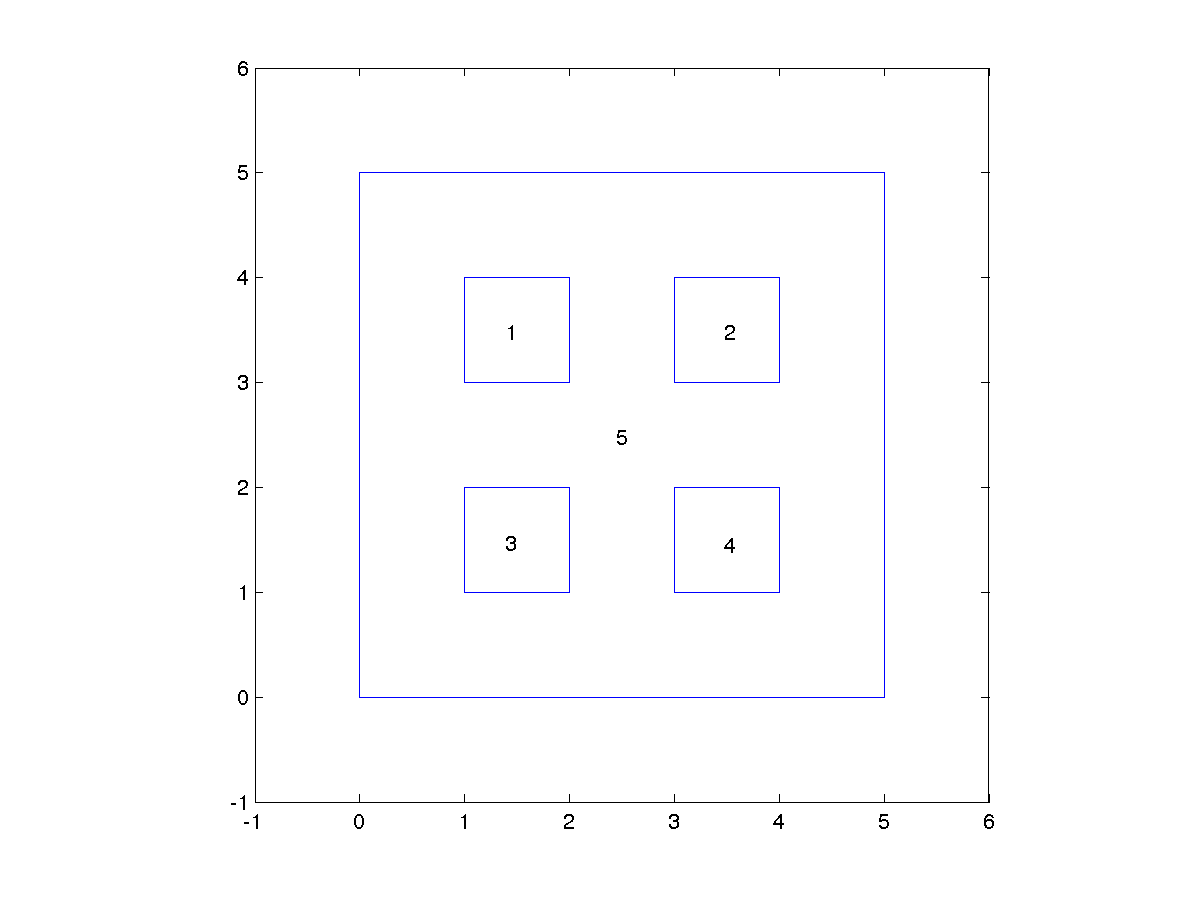
\includegraphics[height=80mm]{4holegeometry}
\caption{Geometry of the model.}\label{fg:4holegeometry}
\end{figure}


\begin{table}[h]
\caption{Material parameters.}
\label{tb:glasspar}
\begin{center}
\begin{tabular}{ll} \hline
parameter  & value \\ \hline
relative permittivity & 7      \\ \hline
\end{tabular}
\end{center}
\end{table} 


\end{flushleft}

\subsection*{Solution procedure}

\begin{flushleft}
Let us next introduce the solution procedure of the problem.
The computation mesh has been created with Gambit software and it consists of 15941 elements. The mesh can be convert into Elmer format with the command

\ttbegin
ElmerGrid 7 2 mesh.FDNEUT
\ttend

This command creates the directory {\tt mesh} which contains the mesh files. 

\ttbegin
Header
  Mesh DB "." "mesh"
End
\ttend

The simulation of the problem is carried out in a 2D Cartesian geometry.
The different permutation are computed within the non-linear iterations of the solver and therefore only one
steady state iteration is needed.

\ttbegin
Simulation
  Coordinate System = "Cartesian 2D"
  Simulation Type = "Steady"
  Output Intervals(1) = 1 
  Steady State Max Iterations = 1
  Output File = File "4_holes.result"
  Post File =   File "4_holes.ep"
End
\ttend

In the solver section the keyword {\tt Calculate Capacitance Matrix} must be set to {\tt True}. 
We also have to define the number of the bodies in our system. 
The calculated matrix is saved to file cmatrix.dat.

\ttbegin
Solver 1
  Equation = "Stat Elec Solver"
  Procedure = "StatElecSolve" "StatElecSolver"
  Variable = "Potential"
  Variable DOFs = 1
  Calculate Capacitance Matrix = Logical True
  Capacitance Bodies = 4
  Minimum CoEnergy = 1e-10
  Capacitance Matrix Filename = "cmatrix.dat"
  Linear System Convergence Tolerance = 1.0E-8
  Linear System Solver = "Iterative"
  Linear System Iterative Method = "BiCGStab"
  Linear System Max Iterations = 1000
  Linear System Abort Not Converged = True
  Linear System Preconditioning = ILU2
  Linear System Residual Output = 1
  Nonlinear System Convergence Tolerance =  1.0E-06
  Nonlinear System Max Iterations = 1
  Nonlinear System Relaxation Factor = 1.0
  Steady State Convergence Tolerance =  1.0E-04
End
\ttend

The body section is defined as follows

\ttbegin
Body 1
  Equation = 1
  Material = 1
End
\ttend                                      

If we want to write the electric energy density in the result file, the keyword {\tt Calculate Electric Energy} has to be set to {\tt True}.      

\ttbegin                                                           
Equation 1
  Active Solvers =  1
  Calculate Electric Energy = Logical True
End
\ttend

We only need one material parameter of glass in our simulation.

\ttbegin               
Material 1
  Relative Permittivity = 7
End
\ttend

The final task is to specify the needed boundary conditions.
The keyword {\tt Capacitance Body} indicates whether the capacitance will be calculated or not.
The bodies, in which the capacitance is going to be computed, should number from 1 up to the value of the
{\tt Capacitance Bodies} in the solver section.
The ground may be given with value 0 for this keyword (or by setting the potential to zero).  

\ttbegin
Boundary Condition 1
  Target Boundaries = 1
  Capacitance Body = 1
End

Boundary Condition 2
  Target Boundaries = 2
  Capacitance Body = 2
End

Boundary Condition 3
  Target Boundaries = 3
  Capacitance Body = 3
End

Boundary Condition 4
  Target Boundaries = 4
  Capacitance Body = 4
End

Boundary Condition 5
  Target Boundaries = 5
  Capacitance Body = 0
End
\ttend

\end{flushleft}


\subsection*{Results}

\begin{flushleft}

Elmer writes the capacitance matrix to file cmatrix.dat.
Note that if the capacitance has been calculated between two different bodies, the calculated value appears two times in the matrix.
Elmer also outputs the calculated capacitances on the screen, where they can be examined:

\begin{center}
\ttbegin
StatElecSolve: Capacitance matrix computation performed (i,j,C_ij)
StatElecSolve:   1  1    2.11054E-10
StatElecSolve:   2  2    2.11027E-10
StatElecSolve:   3  3    2.11015E-10
StatElecSolve:   4  4    2.11052E-10
StatElecSolve:   1  2    7.74093E-11
StatElecSolve:   1  3    7.74260E-11
StatElecSolve:   1  4    1.32739E-11
StatElecSolve:   2  3    1.32801E-11
StatElecSolve:   2  4    7.74067E-11
StatElecSolve:   3  4    7.74120E-11
StatElecSolve: Capacitance matrix was saved to file cmatrix.dat
\ttend 

$Capacitancies$ $(F)$.
\end{center}


\end{flushleft}






























\graphicspath{{./}{InductionHeating/}}
\chapter{Induction heating of a graphite crucible}

\modinfo{Directory}{InductionHeating}
\modinfo{Solvers}{\Idx{StatMagSolve}}
\modinfo{Tools}{\Idx{ElmerGrid}, editor}
\modinfo{Dimensions}{2D, Axi-Symmetric}

\subsection*{Case definition}

At high temperatures the most practical 
method to heat up the crucible 
is by electromagnetic induction. 
The induction coil generates an alternating 
current that flows through the crucible. 
The Ohmic resistance encountered by this current dissipates 
energy, thereby directly
heating the crucible via internal heat generation.

The tutorial case is a simple axi-symmetric crucible that could be
used, for example, to grow silicon carbide (SiC) by the sublimation method.
The crucible 
is made of dense graphite and isolated by 
porous graphite. At the bottom of the crucible there is
some SiC powder. The physical properties of the 
material are given in Table~\ref{tab:ind_heat1}. The dimensions of the
induction heating crucible are given in Table~\ref{tab:ind_heat2}.
Additionally, the powder thickness is 1.0~cm and there are 10 spirals
in the coil.
The frequency of induction heating $f$ is 50 kHz and the current 
$I$ is 10 A.
The permeability of the space is $4\pi 10^{-7}$
if the other variables are in SI-units.

\begin{table}
\caption{Material parameters of the crucible}
\label{tab:ind_heat1}
\begin{center}
\begin{tabular}{llll} \hline
material & $\varepsilon$  & $\kappa$ [W/mk] & $\sigma$ (1/$\Omega$m) \\ \hline 
graphite  &      0.7   &          10.0  &          2.0E4 \\
insulation &      0.9   &          1.0   &          2.0E3  \\
powder    &      0.5   &          25.0  &          1.0E4 \\ \hline
\end{tabular}
\end{center}
\end{table}

\begin{table}
\caption{Dimensions of the crucible}
\label{tab:ind_heat2}
\begin{center}
\begin{tabular}{lllll} \hline
body part &  $r_{inner}$ & $r_{outer}$ & $h_{inner}$ & $h_{outer}$ \\ \hline
graphite  &  2.0   &  2.5 & 6.0 & 8.0 \\
insulation &  2.5   &  4.0 & 8.0 & 12.0 \\
coil      &  5.0   & 5.5  &     & 8.0  \\ \hline
\end{tabular}
\end{center}
\end{table}


\subsection*{Solution Procedure}

At low frequencies the free charges may be neglected and the 
induction heating problem may be solved in terms 
of an magnetic vector potential. The proper solver to do
this is \texttt{StatMagSolver}.
However, the induction heating problem can only be modelled if the helicity 
of the coil is neglected and an average current density is assumed.
This current density may be computed easily when the 
area of the coil is known $j_0=n I / A$, where $A$ is the 
coil area.

The mesh for this problem may easily be created by ElmerGrid.
The provided mesh is quite sufficient for this case
but for higher frequencies the mesh should be tuned 
to solve the thin boundary layers.
The computational mesh is created from file \texttt{crucible.grd} by the 
command 
\ttbegin
ElmerGrid 1 2 crucible
\ttend

The mesh consists of 5 different bodies which need 4
different materials sets. Only one set of boundary conditions 
are required for the external boundary. Thus the header 
information of the command file is as follows
\ttbegin
Header
  Mesh DB "." "crucible"
  Include Path ""
  Results Directory ""
End
\ttend
%
In the \texttt{Simulation} section the coordinate system and
time dependency are set, among other things. Also we know that
the equation is linear and therefore only one steady state
iteration is requited. If the electric properties depend on 
the magnitude of the field then several iterations are required.
\ttbegin
Simulation
  Coordinate System = "Axi Symmetric"
  Simulation Type = Steady State
  Steady State Max Iterations = 1
  Output File = "crucible.result"
  Post File = "crucible.vtu"
End
\ttend
%
In the \texttt{Constants} section the permittivity of 
vacuum must be given.
\ttbegin
Constants
  Permittivity Of Vacuum = 8.8542e-12
End
\ttend
%
In the differential equation for the magnetic vector potential the 
source is the current density. Thus, it is given in the
\texttt{Body Force} section. 
\ttbegin
Body Force 1
  Current Density = 2.5e5
End
\ttend
%
In the \texttt{Body} section the different bodies are assigned 
with correct equation sets and material parameters, for example
\ttbegin
Body 3
  Name = "Insulation"
  Equation = 1
  Material = 2
End
\ttend
%
In the \texttt{Equation} block all the relevant solvers are 
set to active.
\ttbegin
Equation
  Name = "Vector Potential Equation"
  Active Solvers = 1
End
\ttend
%
The only solver in this simple tutorial is the solver for the magnetic
vector potential. Look for the relevant model manual for information
about the options. Here the equation is solved iteratively and the
local Joule heating and magnetic flux are computed as a post processing
step. The Joule heating is scaled so that the total heating power is
3.0~kW. This option may be used when the total heating efficiency is
known.  The nonlinear solver parameters are not really needed as the
material parameters are constant. Sometimes the parameters may depend
on the magnetic field and thus the nonlinear problem must be solved
iteratively.
%
\ttbegin
Solver 1
  Equation = Potential Solver
  Variable = Potential
  Variable DOFs = 2

  Angular Frequency = Real 50.0e3
  Calculate Joule Heating = Logical True
  Calculate Magnetic Flux = Logical True
  Desired Heating = Real 3.0e3

  Procedure = "StatMagSolve" "StatMagSolver"
  Linear System Solver = Iterative
  Linear System Iterative Method = BiCGStab
  Linear System Max Iterations = 300
  Linear System Convergence Tolerance = 1.0e-10
  Linear System Preconditioning = ILU1
  Linear System ILUT Tolerance = 1.0e-03
  Linear System Residual Output = 1
  Nonlinear System Max Iterations = 1
  Nonlinear System Convergence Tolerance = 1.0e-6
  Nonlinear System Relaxation Factor = 1
  Steady State Convergence Tolerance = 1.0e-6
End
\ttend
%
In the \texttt{Material} sections all the necessary 
material parameters are given, for example
\ttbegin
Material 2
  Name = "Insulation"
  Electric Conductivity = 2.0E3
End
\ttend
%
The magnetic field must vanish at infinity. Unfortunately the
computational domain is bounded and therefore the infinite
distance becomes very finite. A proper distance may be checked
by gradually increasing it until no change in the result occurs.
%
\ttbegin
Boundary Condition 1
  Target Boundaries = 1
  Potential 1 = Real 0.0
  Potential 2 = Real 0.0
End
\ttend

\subsection*{Results}

With the given computational mesh the problem is solved in 
a few seconds. With the 20\,072 bilinear elements the heating
efficieny is $16.9$ W. The corresponding results are shown
in Fig.~\ref{fig:ind_heat1}.

\begin{figure}
\begin{center}
  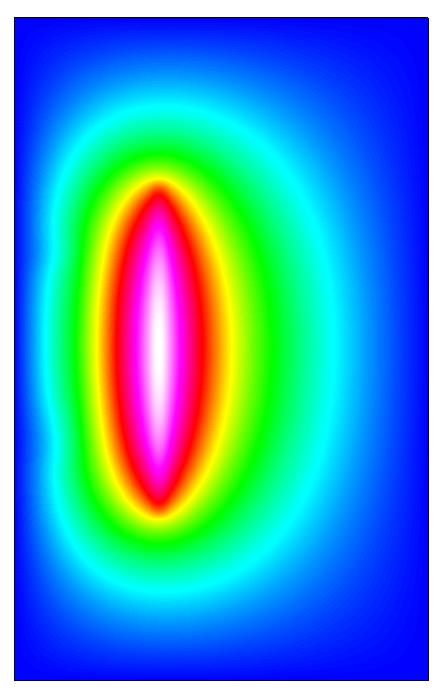
\includegraphics[height=0.4\textwidth]{induct2}
  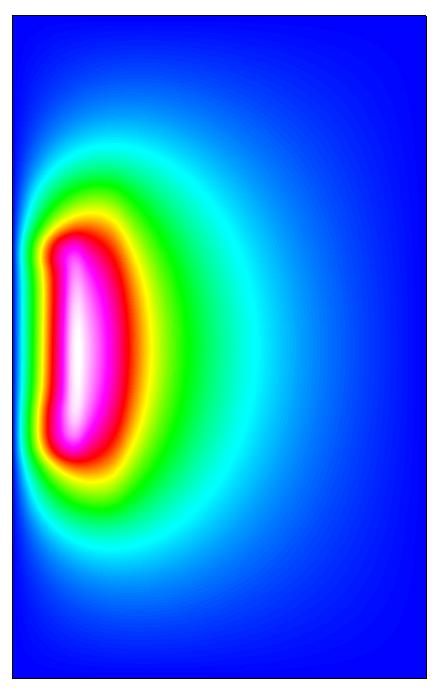
\includegraphics[height=0.4\textwidth]{induct3}
  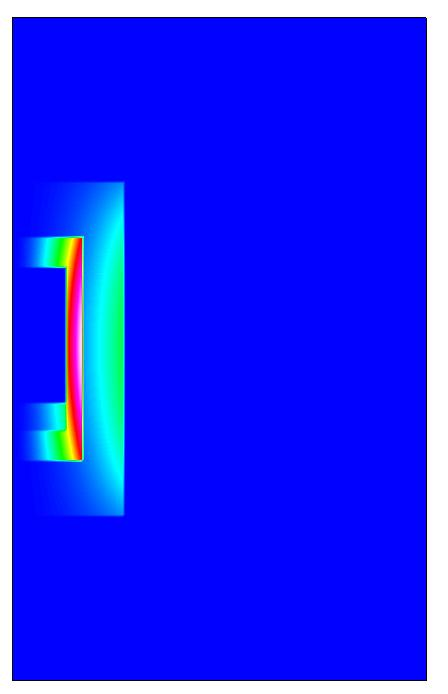
\includegraphics[height=0.4\textwidth]{induct1}
\end{center}
\caption{Induction heating of a simple crucible. 
a) in-phase component of the vector potential
b) out-of-phase component of the vector potential
c) Joule losses in the conductors}
\label{fig:ind_heat1}
\end{figure}



%\graphicspath{{./}{FluidStructureBeam/}}
%\chapter{Fluid flow around an elastic beam}

\modinfo{Directory}{FluiStructureBeam}
\modinfo{Solvers}{\Idx{ElasticSolve}, \Idx{FlowSolve}, \Idx{MeshSolve}}
\modinfo{Tools}{\Idx{ElmerGrid}, editor, \Idx{Fortran 90 compiler}}
\modinfo{Dimensions}{2D, steady-state}

\subsection*{Case definition}

A homogenous, elastic beam ($\Omega_2$) is in a fluid flow (which takes place
in the region $\Omega_1$), 
see figure~\ref{fg:fsi}. The beam is 5.0~m long and it is rigidly 
supported on the end $\Gamma_6$. At the incoming boundary $\Gamma_1$, the 
fluid velocity in the x-direction is a parabola which reaches its 
maximum value 1~m/s at the point y=5.0~m. At the incoming and outcoming 
boundaries $\Gamma_1$ and $\Gamma_2$ velocities in the y-direction 
are 0~m/s. At the outcoming boundary the pressure is 0~Pa. The velocities 
on boundaries $\Gamma_3$, $\Gamma_4$ and $\Gamma_5$ are 0~m/s. The 
fluid is incompressible and has density 1 kg/m$�$, dynamic 
viscosity 0.5 kg/ms and Poisson ratio 0.3. Material properties 
for the beam are the density 1000~kg/m$�$, Poisson ratio 0.3 and Young's 
modulus 1.0e3~N/m$�$. The problem is to solve the maximum displacement 
of the beam and the pressure change in $\Omega_1$.

\begin{figure}[h]
\centering
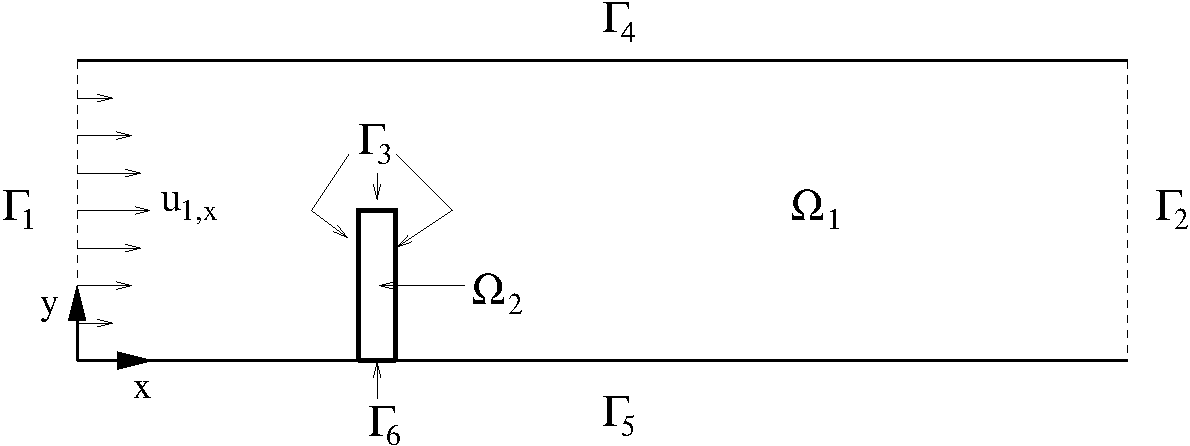
\includegraphics[width=100mm]{fsi}
\caption{Geometry of the problem}\label{fg:fsi}
\end{figure}

The flow generates normal and shear stresses to the beam
boundary $\Gamma_3$. These forces deform the beam and this changes the flow. 
This coupled problem can be modelled using the Navier-Stokes and elasticity 
equations. 

For the incompressible fluid the Navier-Stokes equations can be written as
\begin{equation}
\begin{array}{rcll}
- \nabla \cdot (2 \mu \overline{\overline{\varepsilon}}) + \rho 
\vec{u} \cdot \nabla \vec{u} + \nabla p &=& 0 & \mbox{ in } \Omega_1 \\
\nabla\cdot \vec{u}& = & 0 & \mbox{ in } \Omega_1 \\
\vec{u}_{x} &=& (10y-y^2)/25 & \mbox{ on } \Gamma_1 \\
\vec{u}_{x} &=& 0 & \mbox{ on } \Gamma_i ,\: i=3,4,5 \\
\vec{u}_{y} &=& 0 & \mbox{ on } \Gamma_i ,\: i=1,\ldots,5, 
\end{array}
\end{equation}
where $\mu$ is the dynamic viscosity, $\overline{\overline{\varepsilon}}$ is 
the strain tensor,  $\rho$ is the density, $\vec{u}$ is the velocity vector and
$p$ is the pressure. It is assumed that the density and viscosity are 
constants. 

For the homogeneous, elastic beam the elasticity equations are
\begin{equation}
\begin{array}{rcll}
-div [(I+ \nabla u) \Sigma] &=& 0 & \mbox{ in } \Omega_2 \\
\Sigma &=& \lambda (tr E)I + 2 \mu E & \mbox{ in } \Omega_2 \\
E &=& \frac{1}{2}(\nabla u^{T} + \nabla u + \nabla u^{T} \nabla u) 
& \mbox{ in } \Omega_2 \\
u &=& 0 & \mbox{ on } \Gamma_6 \\
(I+ \nabla u) \Sigma n &=& q & \mbox{ on } \Gamma_3 
\end{array}
\end{equation}
where $u$ is the displacement vector, $\Sigma$ is 
the second Piola-Kirchhoff stress tensor, $\lambda$ and $\mu$ are the Lam\'{e}
constants and $E$ is the Green-St Venant strain tensor, $q$ is the surface 
traction and $n$ is the unit normal to the beam boundary. The edge load $q$ is 
calculated from the stresses obtained using the Navier-Stokes equations.

For updating the fluids mesh a linear elasticity equation is used. In 
mathematical form it can be written as, 
\begin{equation}
\begin{array}{clcr}
-div \{\lambda tr [\varepsilon(v)]I + 2 \mu \varepsilon(v)\} = 0 & 
\mbox{ in } \Omega_1 \\
v = u_{\vert\Gamma_3} & \mbox{ on } \Gamma_3 \\
v = 0 & \mbox{ on } \Gamma_i, i=1,2,4,5 
\end{array}
\end{equation}
where $\lambda$ and $\mu$ are the Lam\'{e} constants, $\varepsilon$ is
linear strain tensor and $v$ is the displacement vector. Here $u$ is the 
solution to the elasticity equations.


\subsection*{Solution procedure}

In this problem geometry and mesh is created by using ElmerGrid by the 
command
\ttbegin
ElmerGrid 1 2 fsi.grd
\ttend

In this problem, external Fortran functions are used to express a
parabolic velocity inflow profile and to define a variable stiffness
for the deforming mesh. The stiffness of the mesh is controlled by the
Youngs modulus. In the case of deforming mesh, the absolute value of
the parameter is not important but its changes over the domain are
influential. The following function defines the mesh to be stiffer
near the corner of the beam where the mesh is deformed most. The idea
is to avoid too irregularly shaped elements in that area.

\ttbegin
FUNCTION Youngs( Model, n, x ) RESULT( s )
  USE Types
  IMPLICIT NONE

  TYPE(Model_t) :: Model
  INTEGER :: n
  REAL(KIND=dp) :: x,s,xx,yy
  
  xx = Model % Nodes % x(n)
  yy = Model % Nodes % y(n)
  
  s =  1.0d0 / SQRT( (xx-11.0)**2 + (yy-4.9)**2 )
  
END FUNCTION Youngs
\ttend

The following function is used to give the inflow boundary condition.

\ttbegin
FUNCTION InFlow( Model, n, x ) RESULT( vin )
  USE Types
  IMPLICIT NONE

  TYPE(Model_t) :: Model
  INTEGER :: n
  REAL(KIND=dp) :: yy,xx,x,vin,v0,vt

  xx = Model % Nodes % x(n)
  yy = Model % Nodes % y(n)
  
  v0 = (-(yy**2)+10*yy)/25
  
  IF(x < 8.0) THEN
    vt = x/8.0
  ELSE
    vt = 1.0
  END IF

  vin = v0*vt

END FUNCTION InFlow
\ttend

In general, the user may supply his/hers own functions for defining
general dependencies of variables or parameters. The function header
should read as follows
\ttbegin
FUNCTION FunctionName( Model, n, x ) RESULT( res )
\ttend
where {\tt Model} is a structure holding various information�of the
problem and {\tt n} is the number of the node being considered. These
are automatically given by the program. The parameter {\tt x} is the
value of the variable, which user defines to be given for the function
as input. The variable is defined in the sif file. Finally, a the
function returns the result {\tt res} for the parameter in
consideration. 

If the Elmer environment is successfully setup the compilation command 
should look like
\ttbegin
elmerf90 -o FsiStuff FsiStuff.f90
\ttend

The functions may be compiled also locally on a PC either for Linux or
WindowsNT, provided that a Fortran90 compiler and the Elmer software
are installed.

The next step is to edit the solver input file (\texttt{sif} file)
with a text editor, {\em e.g.} Emacs.
\begin{itemize}
\item The Header section, where the mesh is defined. 
%
\ttbegin
Header 
  Mesh DB "." "fsi" 
End
\ttend
%
\item The \texttt{Constants} section need not contain any constant this time.
%
\ttbegin
Constants
End
\ttend
%
\item The \texttt{Simulation} section gives the control data for the case.
%
\ttbegin
Simulation
  Coordinate System = Cartesian 2D
  Simulation Type = Steady State
  Steady State Max Iterations = 50
  Steady State Min Iterations = 2
  Output Intervals = 1
  Output File = "fsi.result"
  Post File = "fsi.ep"
End
\ttend
%
\item The \texttt{Body} section is used to define which equations and
materials are used for the simulation bodies.
($\Omega_2$).
%
\ttbegin
Body 1
  Equation = 1
  Material = 1
End

Body 2 
  Equation = 2 
  Material = 2 
End
\ttend
%
\item The \texttt{Material} section defines the material properties of
each body. Also the procedure \texttt{Youngs} is used. 
%
\ttbegin
Material 1 
  Density = 1.0 
  Viscosity = 0.5 
  Poisson Ratio = 0.3 
  Youngs Modulus = Variable time 
      Real Procedure "FsiStuff" "Youngs" 
End

Material 2
   Density = 1000
   Youngs Modulus = 1.0e3
   Poisson Ratio = 0.3
End
\ttend
%
\item The Solver section defines various control parameters for each 
solver.
%
\ttbegin
Solver 1
  Equation = Navier-Stokes
  Stabilize = True
  Linear System Solver = Iterative
  Linear System Iterative Method = BiCGStab
  Linear System Preconditioning = ILU1
  Linear System Max Iterations = 500
  Linear System Convergence Tolerance = 1.0e-8
  Nonlinear System Max Iterations = 10
  Nonlinear System Convergence Tolerance = 1.0e-5
  Nonlinear System Newton After Tolerance = 1.0e-5
  Nonlinear System Newton After Iterations = 20
  Nonlinear System Relaxation Factor = 1.0
  Steady State Convergence Tolerance = 1.0e-4
End

Solver 2
  Equation = Elasticity Solver
  Variable = Displacement
  Variable DOFs = 2
  Procedure = "ElasticSolve" "ElasticSolver"
  Linear System Solver = Direct
  Linear System Direct Method = Banded
  Nonlinear System Newton After Tolerance = 1.0e-3
  Nonlinear System Newton After Iterations = 20
  Nonlinear System Max Iterations = 100
  Nonlinear System Convergence Tolerance = 1.0e-5
  Nonlinear System Relaxation Factor = 1.0
  Steady State Convergence Tolerance = 1.0e-4
End

Solver 3 
  Equation = Mesh Update
  Linear System Solver = Iterative
  Linear System Iterative Method = BiCGStab
  Linear System Preconditioning = ILU1
  Linear System Max Iterations = 500
  Linear System Convergence Tolerance = 1.0e-8
  Steady State Convergence Tolerance = 1.0e-4
End
\ttend
%
\item The \texttt{Equation} section. This section defines the
equations for a body. Plane stress model for the elastic beam is 
applied. Setting this keyword to {\tt False} enables the plane 
strain assumption.
%
\ttbegin
Equation 1
  Active Solvers(2) = 1 3
End

Equation 2
  Active Solvers = 2
  Plane Stress = True
End
\ttend
%
\item In the \texttt{Boundary Condition} section different boundary
conditions are defined.  In Boundary Condition~1 the shape of inflow
is defined with the Fortran procedure \texttt{InFlow}. Note also the
bc 3, where keyword {\tt FSI BC} is supplied to define the boundary on
which the fluid affects a force on the elastic beam. Also, on the same
boundary, the mesh is constraint to follow the deformation of the beam
by the two Equals lines.
%
\ttbegin
Boundary Condition 1 
  Target Boundaries = 1
  Velocity 1 = Variable Time
      Real Procedure "FsiStuff" "InFlow"

  Velocity 2 = 0.0
  Mesh Update 1 = 0.0
End 

Boundary Condition 2
  Target Boundaries = 2
  Velocity 2 = 0.0
  Pressure = 0.0
  Mesh Update 1 = 0.0
End

Boundary Condition 3 
  Target Boundaries = 3
  Velocity 1 = 0.0
  Velocity 2 = 0.0
  FSI BC = True
  Mesh Update 1 = Equals Displacement 1
  Mesh Update 2 = Equals Displacement 2
End

Boundary Condition 4
  Target Boundaries(2) = 4 5
  Velocity 1 = 0.0
  Velocity 2 = 0.0
  Mesh Update 2 = 0.0
End

Boundary Condition 5
  Target Boundaries = 6 
  Displacement 1 = 0.0
  Displacement 2 = 0.0
End
\ttend
%
\end{itemize}

\subsection*{Results}

After the solution is done, view the results with ElmerPost. 
Read the result file fsi.ep in ElmerPost by choosing Read Model File. The 
fsi.ep file is located in the same directory as the mesh files. 

\begin{table}[tbhp]
\caption{Max. displacement and pressure difference}
\label{tb:struct5}
\begin{center}
\begin{tabular}{lll} \hline
Elements & $\max |u|$ [m] & $\max \Delta p$ [Pa] \\  \hline 
540  &  1.34  &  6.36  \\ \hline 
\end{tabular}
\end{center}
\end{table}

As a result the maximum absolute value of displacement and the 
pressure difference is given (see table~\ref{tb:struct5}).


\graphicspath{{./}{ThermalActuator/}}
\chapter{Thermal actuator driven with electrostatic currents}

\modinfo{Test}{ThermalActuator}
\modinfo{Directory}{ThermalActuator}
\modinfo{Solvers}{\Idx{StatCurrentSolve}, \Idx{HeatSolve}, 
	\Idx{StressSolve}}
\modinfo{Tools}{\Idx{ElmerGrid}, editor}
\modinfo{Dimensions}{3D, Steady-state}

\subsection*{Case definition}

The tutorial introduces a micro mechanical thermal actuator as shown
in Fig.~\ref{geom_thermal}. A static electric current is driven
through the actuator. The power loss due to the resistance of the
actuator is transformed into heat which in turn causes thermal
stresses into the structure. The electric current thus results in
deformation of the actuator. In industry, such an actuator might be
used to control the position of a micromechanical component.

\begin{figure}[h]
  \centerline{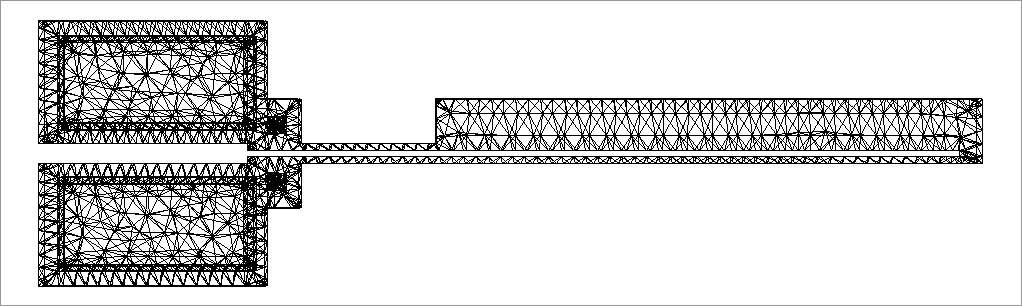
\includegraphics[width=0.8\textwidth]{geometry_wh}}
  \caption{The geometry of the actuator.} 
  \label{geom_thermal}
\end{figure}


\subsection*{Solution procedure}

The problem is solved by first iterating the electrostatic current
solver and heat equation until both are converged. The temperature
distribution is then used as a load for stress analysis solver which
calculates the actual deformation of the structure. The electric
conductivity of the actuator depends on the temperature and thus the
electrostatic - thermal problem is coupled in both directions.

The computational mesh for this particular tutorial is created by
using \Idx{Ansys} software. The details of the mesh are written into
files called \texttt{ExportMesh} by a certain Ansys macro and
converted to Elmer format by the ElmerGrid program. The command to use
is
\ttbegin
ElmerGrid 4 2 ExportMesh -order 1.0 0.1 0.001 -o thermal
\ttend 
The above command reads in the Ansys mesh files, arranges the mesh 
nodes in a reasonable way and saves the mesh in Elmer format in a
directory called \texttt{thermal}.

The geometry of the problem includes only one body and
material. Boundary conditions are defined on the actuator legs, which
are kept at constant electric potential, temperature and
position. Thus, only Dirichlet boundary conditions are used.

The header and simulation blocks of the solver input file are

\ttbegin
Header
  Mesh DB "." "thermal"
End

Simulation
  Coordinate System = Cartesian 3D
  Simulation Type = Steady State
  Steady State Max Iterations = 30
  Output Intervals = 1
  Output File = "actuator.result"
  Post File = "actuator.vtu"
End
\ttend

An initial condition for temperature is defined in order to ease the
convergence of the iterative solvers. Also, a body force for the
heat equation solver defining the Joule heating is needed. These
both have to be declared in the body section as follows:

\ttbegin
Body 1
  Equation = 1
  Material = 1
  Initial Condition = 1
  Body Force = 1
End
\ttend

The solution procedure requires the use of three solvers: Static
current solver, heat equation solver and the stress analysis
solver. The equation block below defines that these solvers are
used. 

\ttbegin
Equation 1
  Active Solvers(3) = Integer 1 2 3
  Calculate Joule Heating = True
End
\ttend

The solver blocks define the parameters of the respecting solvers. The
static current conduction problem is tackled by an iterative conjugate
gradient method (CG). For heat equation, a stabilized biconjugate
gradient method is used. The coupled problem of these two solvers is
difficult since the static current calculated heats the structure on
each step, and the rise of temperature makes the current conduction
more and more difficult. To overcome this problem, a relaxation factor
of 0.5 is defined for the heat equation solver.

\ttbegin
Solver 1
  Equation = Stat Current Solver
  Procedure = "StatCurrentSolve" "StatCurrentSolver"
  Variable = Potential
  Variable DOFs = 1
  Calculate Volume Current = True
  Calculate Electric Conductivity = True
  Linear System Solver = Iterative
  Linear System Iterative Method = CG
  Linear System Preconditioning = ILU3
  Linear System Max Iterations = 300
  Linear System Convergence Tolerance = 1.0e-8
  Nonlinear System Max Iterations = 1
  Nonlinear System Convergence Tolerance = 1.0-6
  Nonlinear System Newton After Iterations = 3
  Nonlinear System Newton After Tolerance = 1.0e-12
  Nonlinear System Relaxation Factor = 1.0
  Steady State Convergence Tolerance = 1.0e-6
End

Solver 2
   Equation = Heat Equation
   Variable = Temperature
   Variable DOFs = 1
   Linear System Solver = Iterative
   Linear System Iterative Method = BiCGStab
   Linear System Preconditioning = ILU1
   Linear System Max Iterations = 350
   Linear System Convergence Tolerance = 1.0e-9
   Nonlinear System Max Iterations = 1
   Nonlinear System Convergence Tolerance = 1.0e-07
   Nonlinear System Newton After Iterations = 3
   Nonlinear System Newton After Tolerance = 1.0e-12
   Nonlinear System Relaxation Factor = 0.5
   Steady State Convergence Tolerance = 1.0e-07
End
\ttend

For stress analysis, a direct solver is used instead of an iterative
solver. It is often difficult for the iterative solver to find a
solution for a structure that contains parts with varying stiffness
properties, which is obviously the case here (try the iterative solver
and see!). The stress analysis solver is called first only after the
coupled iteration of two previous solvers is complete. This is
possible since the deformation of the structure is so small that it
does not change the current density distribution. Defining stress
analysis this way saves computational time. It is possible to
iterate all the three solvers until convergence by commenting the
\texttt{Exec Solver} line.

\ttbegin
Solver 3
  Exec Solver = After All
  Equation = Stress Analysis
  Variable = Displacement
  Variable DOFs = 3
  Linear System Solver = Direct
  Linear System Direct Method = Banded
  Nonlinear System Max Iterations = 1
  Nonlinear System Convergence Tolerance = 1.0e-6
  Nonlinear System Newton After Iterations = 3
  Nonlinear System Newton After Tolerance = 1.0e-12
  Nonlinear System Relaxation Factor = 1.0
  Steady State Convergence Tolerance = 1.0e-6
End
\ttend

The material of the structure has a temperature dependent electric
conductivity. This, as well as other material parameters, is defined
in the material block. Note that a MEMS unit system is used.

\ttbegin
Material 1
  Electric Conductivity = Variable Temperature
      Real
        298.0   4.3478e10
        498.0   1.2043e10
        698.0   5.1781e9
        898.0   2.7582e9
        1098.0  1.6684e9
        1298.0  1.0981e9
        1683.0  1.0
        2000.0  1.0
      End

  Density = 2.3e-15
  Heat Conductivity = 32.0e6
  Youngs Modulus = 169.0e3
  Poisson Ratio = 0.22
  Heat Expansion Coefficient = 2.9e-6
  Reference Temperature = 298.0
End
\ttend

Finally, the initial condition, thermal heat load for stress analysis,
and the boundary conditions are defined.

\ttbegin
Initial Condition 1
   Temperature = 298.0
End

Body Force 1
  Heat Source = Equals Joule Heating
End

Boundary Condition 1
  Target Boundaries = 1
  Potential = 0
  Temperature = 298
  Displacement 1 = 0.0
  Displacement 2 = 0.0
  Displacement 3 = 0.0
End

Boundary Condition 2
  Target Boundaries = 2
  Potential = 7
  Temperature = 298
  Displacement 1 = 0.0
  Displacement 2 = 0.0
  Displacement 3 = 0.0
End
\ttend

\subsection*{Results}

The problem converges after 27 steady state iterations on the
tolerance limits defined above. The calculation takes about 180 cpu
seconds of which 40 cpus is spent in solving the stress analysis
equation. The calculations were performed on a Compaq Alpha Server
with a 1 GHz central processor.

\begin{figure}[tbhp]
  \centerline{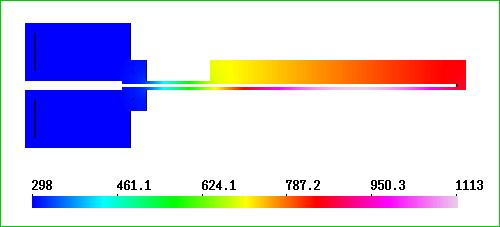
\includegraphics[width=0.8\textwidth]{temp_wh}}
  \caption{Temperature distribution.} 
  \label{temp_thermal}
\end{figure}
\begin{figure}[h]
  \centerline{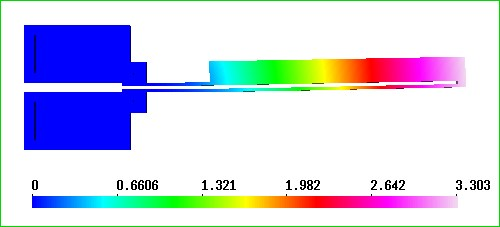
\includegraphics[width=0.8\textwidth]{displ_wh}}
  \caption{The displacement of the actuator.} 
  \label{displ_thermal}
\end{figure}

Result for temperature distribution and the displacement are shown in
Figs~\ref{temp_thermal} and~\ref{displ_thermal}. The temperature rises
unrealistically high in this example because all heat transfer
mechanisms out of the structure are neglected. Presumably at least
the heat radiation is of major importance in this case. For
displacement, the results show a movement of about 3.3 micrometers for
the actuator tip.

\vfill
\mbox{}


\graphicspath{{./}{CoatingProcess/}}
\chapter{Axisymmetric coating process}

\modinfo{Director}{CoatingProcess}
\modinfo{Solvers}{\Idx{FlowSolve}, \Idx{FreeSurfaceReduced}}
\modinfo{Tools}{\Idx{ElmerGrid}, editor}
\modinfo{Dimensions}{2D, Steady-state}

\subsection*{Case definition}

The optical fibers are quite fragile and must therefore be coated with
a layer of polymer before they are stored.  This means that the
coating process must be done with the same speed as the drawing of
optical fibers.  When the diameter of the fiber is only 125 $\mu$m
this sets high demands for the coating geometry since it must provide
even coating at high draw speeds. In Elmer a tailored free surface
boundary condition allows an efficient solution of this particular
problem.


\subsection*{Solution procedure}

The mesh is done with ElmerGrid in the directory coat by the command
%
\ttbegin
ElmerGrid 1 2 coat.grd
\ttend

Therefore the header reads 
\ttbegin
Header
  Mesh DB "." "coat"
End
\ttend
%
The geometry is axisymmetric and the problem is solved in steady state. Typically around 10
iterations is needed to solve the problem but to be on the safe side 30 is set as the maximum.
\ttbegin
Simulation
  Coordinate System = Axi Symmetric
  Simulation Type = Steady State
  Steady State Max Iterations = 30
  Output Intervals = 1
  Output File = "coat.result"
  Post File = "coat.vtu"
End
\ttend
%
In this case there is only one body which comprises of the polymer 
floating between the coating cup and the optical fiber.
\ttbegin
Body 1
  Equation = 1
  Material = 1
End
\ttend

The presented solution used four different solvers. 
The Navier-Stokes solver is required to solve the flow field
for the polymer.
\ttbegin
Solver 1
  Equation = Navier-Stokes
  Stabilize = True
  Internal Move Boundary = Logical False
  Nonlinear System Max Iterations = 5
  Nonlinear System Convergence Tolerance = 1.0e-7
  Nonlinear System Newton After Iterations = 2
  Nonlinear System Newton After Tolerance = 1.0e-2
  Nonlinear System Relaxation Factor = 0.7
  Linear System Solver = Iterative
  Linear System Iterative Method = BiCGStab 
  Linear System Preconditioning = ILU1
  Linear System Max Iterations = 100
  Linear System Convergence Tolerance = 1.0e-10
  Steady State Convergence Tolerance = 1.0e-7
End
\ttend
%
A tailored free surface solver is used to find the 
position of the free surface with a given flow field.
The variable being solved is the displacement of the free surface.
Relaxation is used to avoid over-shooting during the itaration.
This solver does not solve any matrix equations. Instead it solves
the radius from the mass conservation constraint for each node on the
free surface separately. There is a possibility to do the mapping also 
within the solver using a 1D scheme but this is disabled by setting
the \texttt{Perform Mapping} to be \texttt{False}.
\ttbegin
Solver 2
  Equation = "Free Surface Reduced"
  Procedure = "FreeSurfaceReduced" "FreeSurfaceReduced"
  Variable = Dx
  Variable DOFs = 1
  Nonlinear System Relaxation Factor = 0.7
  Nonlinear System Convergence Tolerance = 1.0e-3
  Steady State Convergence Tolerance = 1.0e-3
  Perform Mapping = Logical False
End
\ttend
%
The mesh update solver is required to map the computational mesh
so that it corresponds to the altered geometry.
Here the displacements of the free surface have already been computed
and this solver solves the displacements inside the domain.
Note that solvers 1, 2 and 3 are coupled and therefore the system must be solved iteratively
\ttbegin
Solver 3
  Equation = Mesh Update
  Linear System Solver = Iterative 
  Linear System Iterative Method = BiCGSTAB
  Linear System Preconditioning = ILU
  Linear System Convergence Tolerance = 1.0e-12
  Linear System Max Iterations = 200
  Linear System Symmetric = True
  Steady State Convergence Tolerance = 1.0e-4
End
\ttend
%
In the end, an additional solver is used to compute the forces
acting on the fiber. This does not affect the results.
\ttbegin
Solver 4 
  Equation = Fluidic Force
  Procedure = "FluidicForce" "ForceCompute"
  Calculate Viscous Force = Logical True
End
\ttend
%
Additionally there are two solvers for saving the results in a form
that is more useful than plain pictures. The \texttt{SaveScalars} saves
the scalar values, such as the diameter and force values,
and the \texttt{SaveLine} saves the free surface.
\ttbegin
Solver 5
  Equation = SaveScalars
  Procedure = "SaveData" "SaveScalars"
  Filename = "scalars.dat"
End 

Solver 6
  Equation = SaveLine
  Procedure = "SaveData" "SaveLine"
  Filename = "kurvi.dat"
End
\ttend
%
The equation includes only the solvers that need a permutation vector 
pointing out the active nodes. Therefore the save utilities do not need to belong
to the set of active solvers.
\ttbegin
Equation 1
  Active Solvers(4) = 1 2 3 4
End
\ttend
%
The material parameters are those of the polymer. Additionally elasticity 
parameters are needed because the solver that updates the mesh is actually
a linear elasticity solver.
\ttbegin
Material 1
  Density = 1.0
  Viscosity = 1.0
  Poisson Ratio = 0.3
  Youngs Modulus = 1.0
End
\ttend

Five different boundary conditions are needed.
The origin is a symmetry axis and therefore the radial velocity is 
set to zero. The axial velocity is the draw velocity.
\ttbegin
Boundary Condition 1
  Name = "Symmetry"
  Target Boundaries = 1
  Velocity 2 = -10.0     ! The draw velocity
  Velocity 1 = 0.0
  Compute Fluidic Force = Logical True
  Mesh Update 1 = 0.0
End
\ttend
%
The free surface has a condition stating that the reduced order free 
surface solver should be solved for that. Additionally the 
free surface is a boundary condition for the mesh update,
and a line to be saved.
\ttbegin
Boundary Condition 2
  Name = "Free"
  Target Boundaries = 2
  Mesh Update 1 = Equals Dx
  Mesh Update 2 = 0.0
  Free Surface Reduced = Logical True
  Save Line = Logical True
End
\ttend
%
At the outlet the radial velocity should vanish and the axial coordinate should
be fixed.
\ttbegin
Boundary Condition 3
  Name = "Outlet"
  Target Boundaries = 3
  Velocity 1 = 0.0
  Mesh Update 2 = 0.0
End
\ttend
%
At the inlet it is assumed that there is no radial velocity and that 
the pressure acting on the surface is zero.
\ttbegin
Boundary Condition 4
  Name = "Inlet"
  Target Boundaries = 4
  Velocity 1 = 0.0
  Pressure = 0.0
  Mesh Update 2 = 0.0
End
\ttend
%
Finally, no-slip conditions are set for the boundaries with the walls of the
coater.
\ttbegin
Boundary Condition 5
  Name = "No-slip"
  Target Boundaries = 5
  Velocity 1 = 0.0
  Velocity 2 = 0.0
  Mesh Update 1 = 0.0
  Mesh Update 2 = 0.0
End
\ttend


\subsection*{Results}

\begin{figure}[tbhp]
\begin{center}
  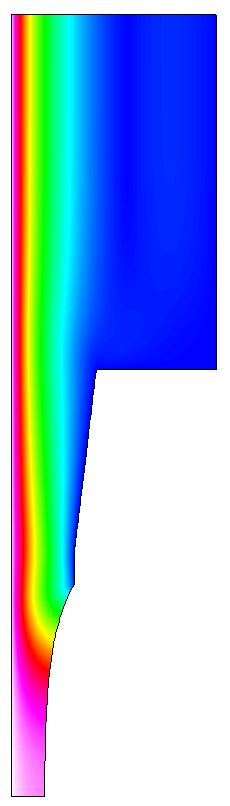
\includegraphics[height=0.6\textwidth,angle=0]{coat_vel}
  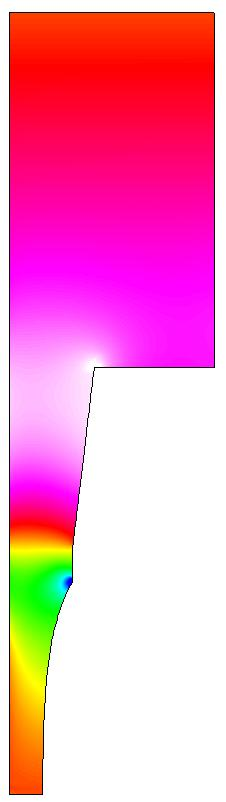
\includegraphics[height=0.6\textwidth,angle=0]{coat_pres}
  \caption{The velocity and pressure fields in a simple coating geometry.
	The solution utilizes the reduced dimensional free surface solver.}
\end{center}
\end{figure}

In the given case solution is obtained after 13 iterations.
The solution gives the final radius, the forces, and the profile of the 
free surface. To visualize the true free surface you may visualize the
last time step using Paraview, or some other software capable of reading
VTU files. 
%ead in the only the last timestep and in \texttt{ElmerPost} give the following
%ommands:
%ttbegin
%ath nodes0 = nodes
%ath nodes = nodes0 + Mesh.Update
%ttend
%ote that this does not work if there is more than one set of variable values.


\vfill
\mbox{}


\graphicspath{{./}{ArteryFlow/}}
\chapter{Blood ejection from a ventricle into aorta}

\modinfo{Test}{ArteryOutlet}
\modinfo{Directory}{ArteryFlow}
\modinfo{Solvers}{\Idx{FlowSolve},\Idx{ElasticSolve}, \Idx{OutletCompute}} 
\modinfo{Tools}{Editor, \Idx{Fortran 90 compiler}, \Idx{ElmerGrid}}
\modinfo{Dimensions}{2D, Transient}

\subsection*{Case description}

This tutorial is about simulating blood ejection in to the elastic human aorta.
The idea is to mimic left ventricle contraction and resulting pulse propagation 
in an elastic conduit. In the simulation about 0.8 
deciliters of blood is ejected to a 50 cm long elastic aorta during a time 
period of 400 ms.  In order to get the outlet of the model behave 
physiologically more realistic way, a one dimensional model is coupled
with the higher order model.
 
\subsection*{Solution procedure}

First we generate the mesh of 366 eight-node quadrilaterals elements with 
the command
\ttbegin
ElmerGrid 1 2 contra
\ttend
Next we generate one dimensional mesh to the outlet of the 2D model.
The program {\tt AddOneDim} is posed to be run in the mesh directory
{\tt contra}.  The length, the number of the elements, 
and the coordinate direction of the 1D section will be asked.

In the simulation block the timestep is set equal to 1 ms and 
total simulation time equal to 600 ms.  The geometry consists of five bodies
of which the first three are for the fluid volume.  Body number 1 os the 
contracting volume.  Body 2 is a short rigid channel between the body 1 and 
the elastic artery. Artificial compressibility
method is used for the fluid volume (body 3) which is in contact with the 
elastic wall (body 4).  One dimensional model is the body 5. 
Material settings for those are 
following:
\ttbegin
! Bodies 1 and 2 (blood)
Material 1
  Density = 1000
  Viscosity = 3.5e-3
  Youngs Modulus = 1
  Poisson Ratio = 0.3
End

! Body 3 (blood)
Material 2
  Density = 1000
  Viscosity = 3.5e-3
  Youngs Modulus = 1
  Poisson Ratio = 0.3
  Compressibility Model = Artificial Compressible
  Artificial Compressibility  = 3.3E-5 
End

! Body 4 (elastic wall)
Material 3
  Density = 1010
  Youngs Modulus = 3.0e5
  Poisson Ratio = 0.45
End

! One dimensional model
Material 4
   Density = 1010.0
   Artery Wall Youngs Modulus = Real 3.0e5 
   Artery Radius = Real 0.0135 
   Artery Wall Thickness = Real 0.002
   Artery Poisson Ratio  = Real 0.45
End
\ttend

Notice that the radius of the one dimensional model ({\tt Artery Radius})
is to the midplane of the wall (inner radius + half of the wall thickness).
The overall FSI iteration scheme is started by one dimensional solver
({\tt OutletCompute}, see the solver manual), after that Navier-Stokes, 
elasticity and mesh update solvers are run.  Steady state convergence tolerance
is set equal to 1.0E-4 for each of the solvers.  The nonlinearities
of each of the solvers are computed within the FSI scheme loop, that is,
the flag {\tt Nonlinear System Max Iterations} is set equal to 1.
Artificial compressibility coefficient is computed by the equation
$c = (1-\nu^2) [D/(E~h)]$, where $\nu$ is the Poisson ratio of the
artery wall, $D$, $E$ and $h$ are the inner diameter, Young's modulus
and the thickness of the artery, respectively.

The only driving force of the system, the wall motion of the contracting 
fluid domain is given by the fortran function {\tt Motion}, see the
figure \ref{fig:contra}.  The boundary condition setting is
\ttbegin
! Moving boundary
Boundary Condition 1
  Target Boundaries = 1
  Velocity 1 = 0
  Velocity 2 = Equals Mesh Velocity 2
  Mesh Update 1 = Real 0
  Mesh Update 2 = Variable Time
       Real Procedure "./Motion" "Motion"
End
\ttend

At the outlet, the pressure boundary condition is given by the
function {\tt OutletPres} and the corresponding radial displacement
of the end wall of the outlet is given by the function {\tt OutletdX}
\ttbegin
! Outlet pressure of the 2D model
Boundary Condition 2
  Target Boundaries = 2
  Flux Integrate = Logical True
  Flow Force BC = True
  Pressure 2 = Variable Time
      Real Procedure "./ArteryOutlet" "OutletPres"
  Mesh Update 2 = Real 0
End

! Radial displacement of the end wall at the outlet of 2D model
Boundary Condition 9
  Target Boundaries = 9
  Displacement 1 = Variable Time
      Real Procedure "ArteryOutlet" "OutletdX"
  Displacement 2 = 0 
End
\ttend
FSI interface boundary is described as following
\ttbegin
! FSI interface boundary
Boundary Condition 11
  Target Boundaries = 11
  Velocity 1 = Equals Mesh Velocity 1
  Velocity 2 = Equals Mesh Velocity 2
  Mesh Update 1 = Equals Displacement 1
  Mesh Update 2 = Equals Displacement 2
  Force BC = Logical True
End
\ttend
Finally, the coupling of the 1D model with the 2D is 
done at the inlet boundary as
\ttbegin
Boundary Condition 16
  Target Boundaries = 16
  Fluid Coupling With Boundary = Integer 2
  Structure Coupling With Boundary = Integer 9
End
\ttend


\subsection*{Results}

The contraction is curve seen in the figure \ref{fig:contra} and
the velocity fields at different time levels are presented
in the figure~\ref{fig:velofields}.  Postprocessing instructions
are given in the file {\tt PostProcessingInstr.txt}.

\begin{figure}[!hb]
\begin{center}
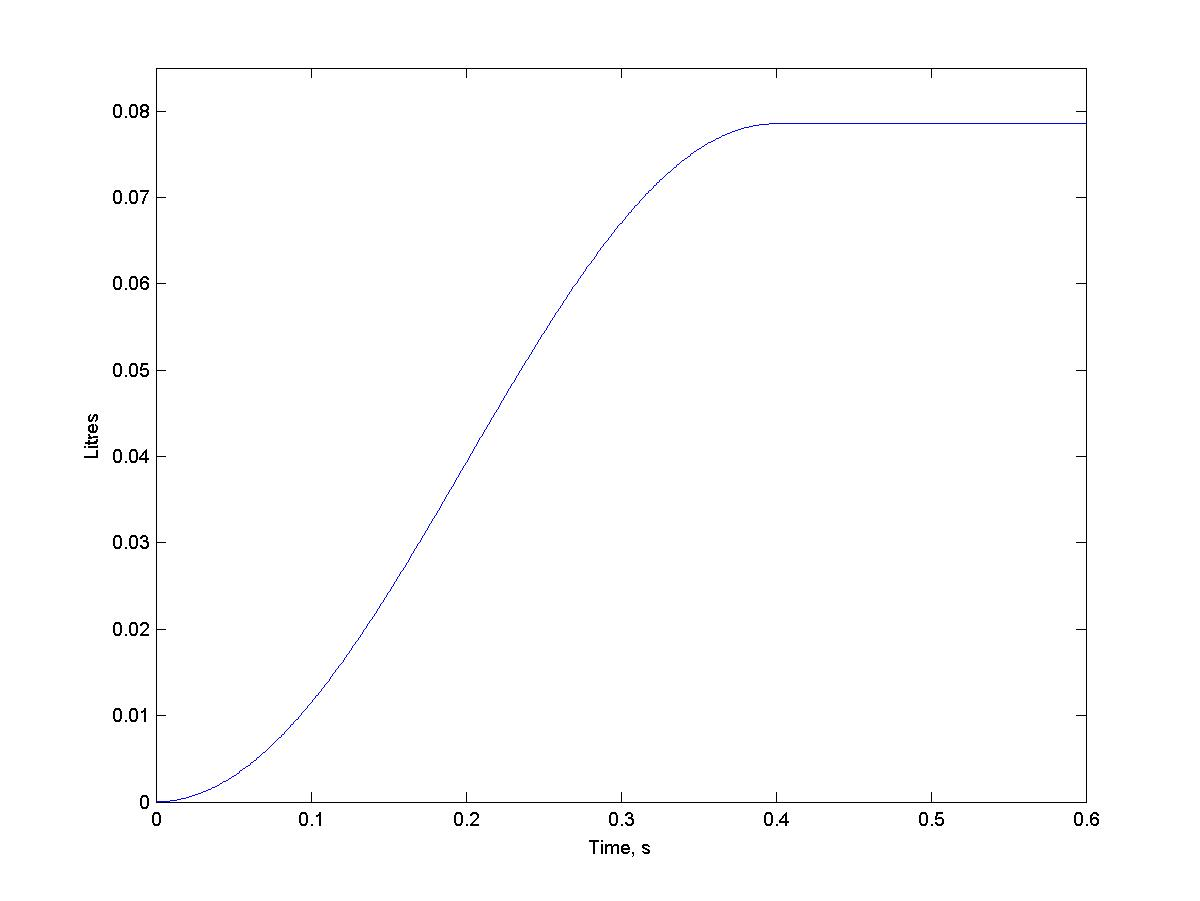
\includegraphics[width=15cm]{motion}
\caption{Contraction curve generated by the function {\tt Motion}.}
\label{fig:contra}
\end{center}
\end{figure}

\begin{figure}[!hb]
\begin{center}
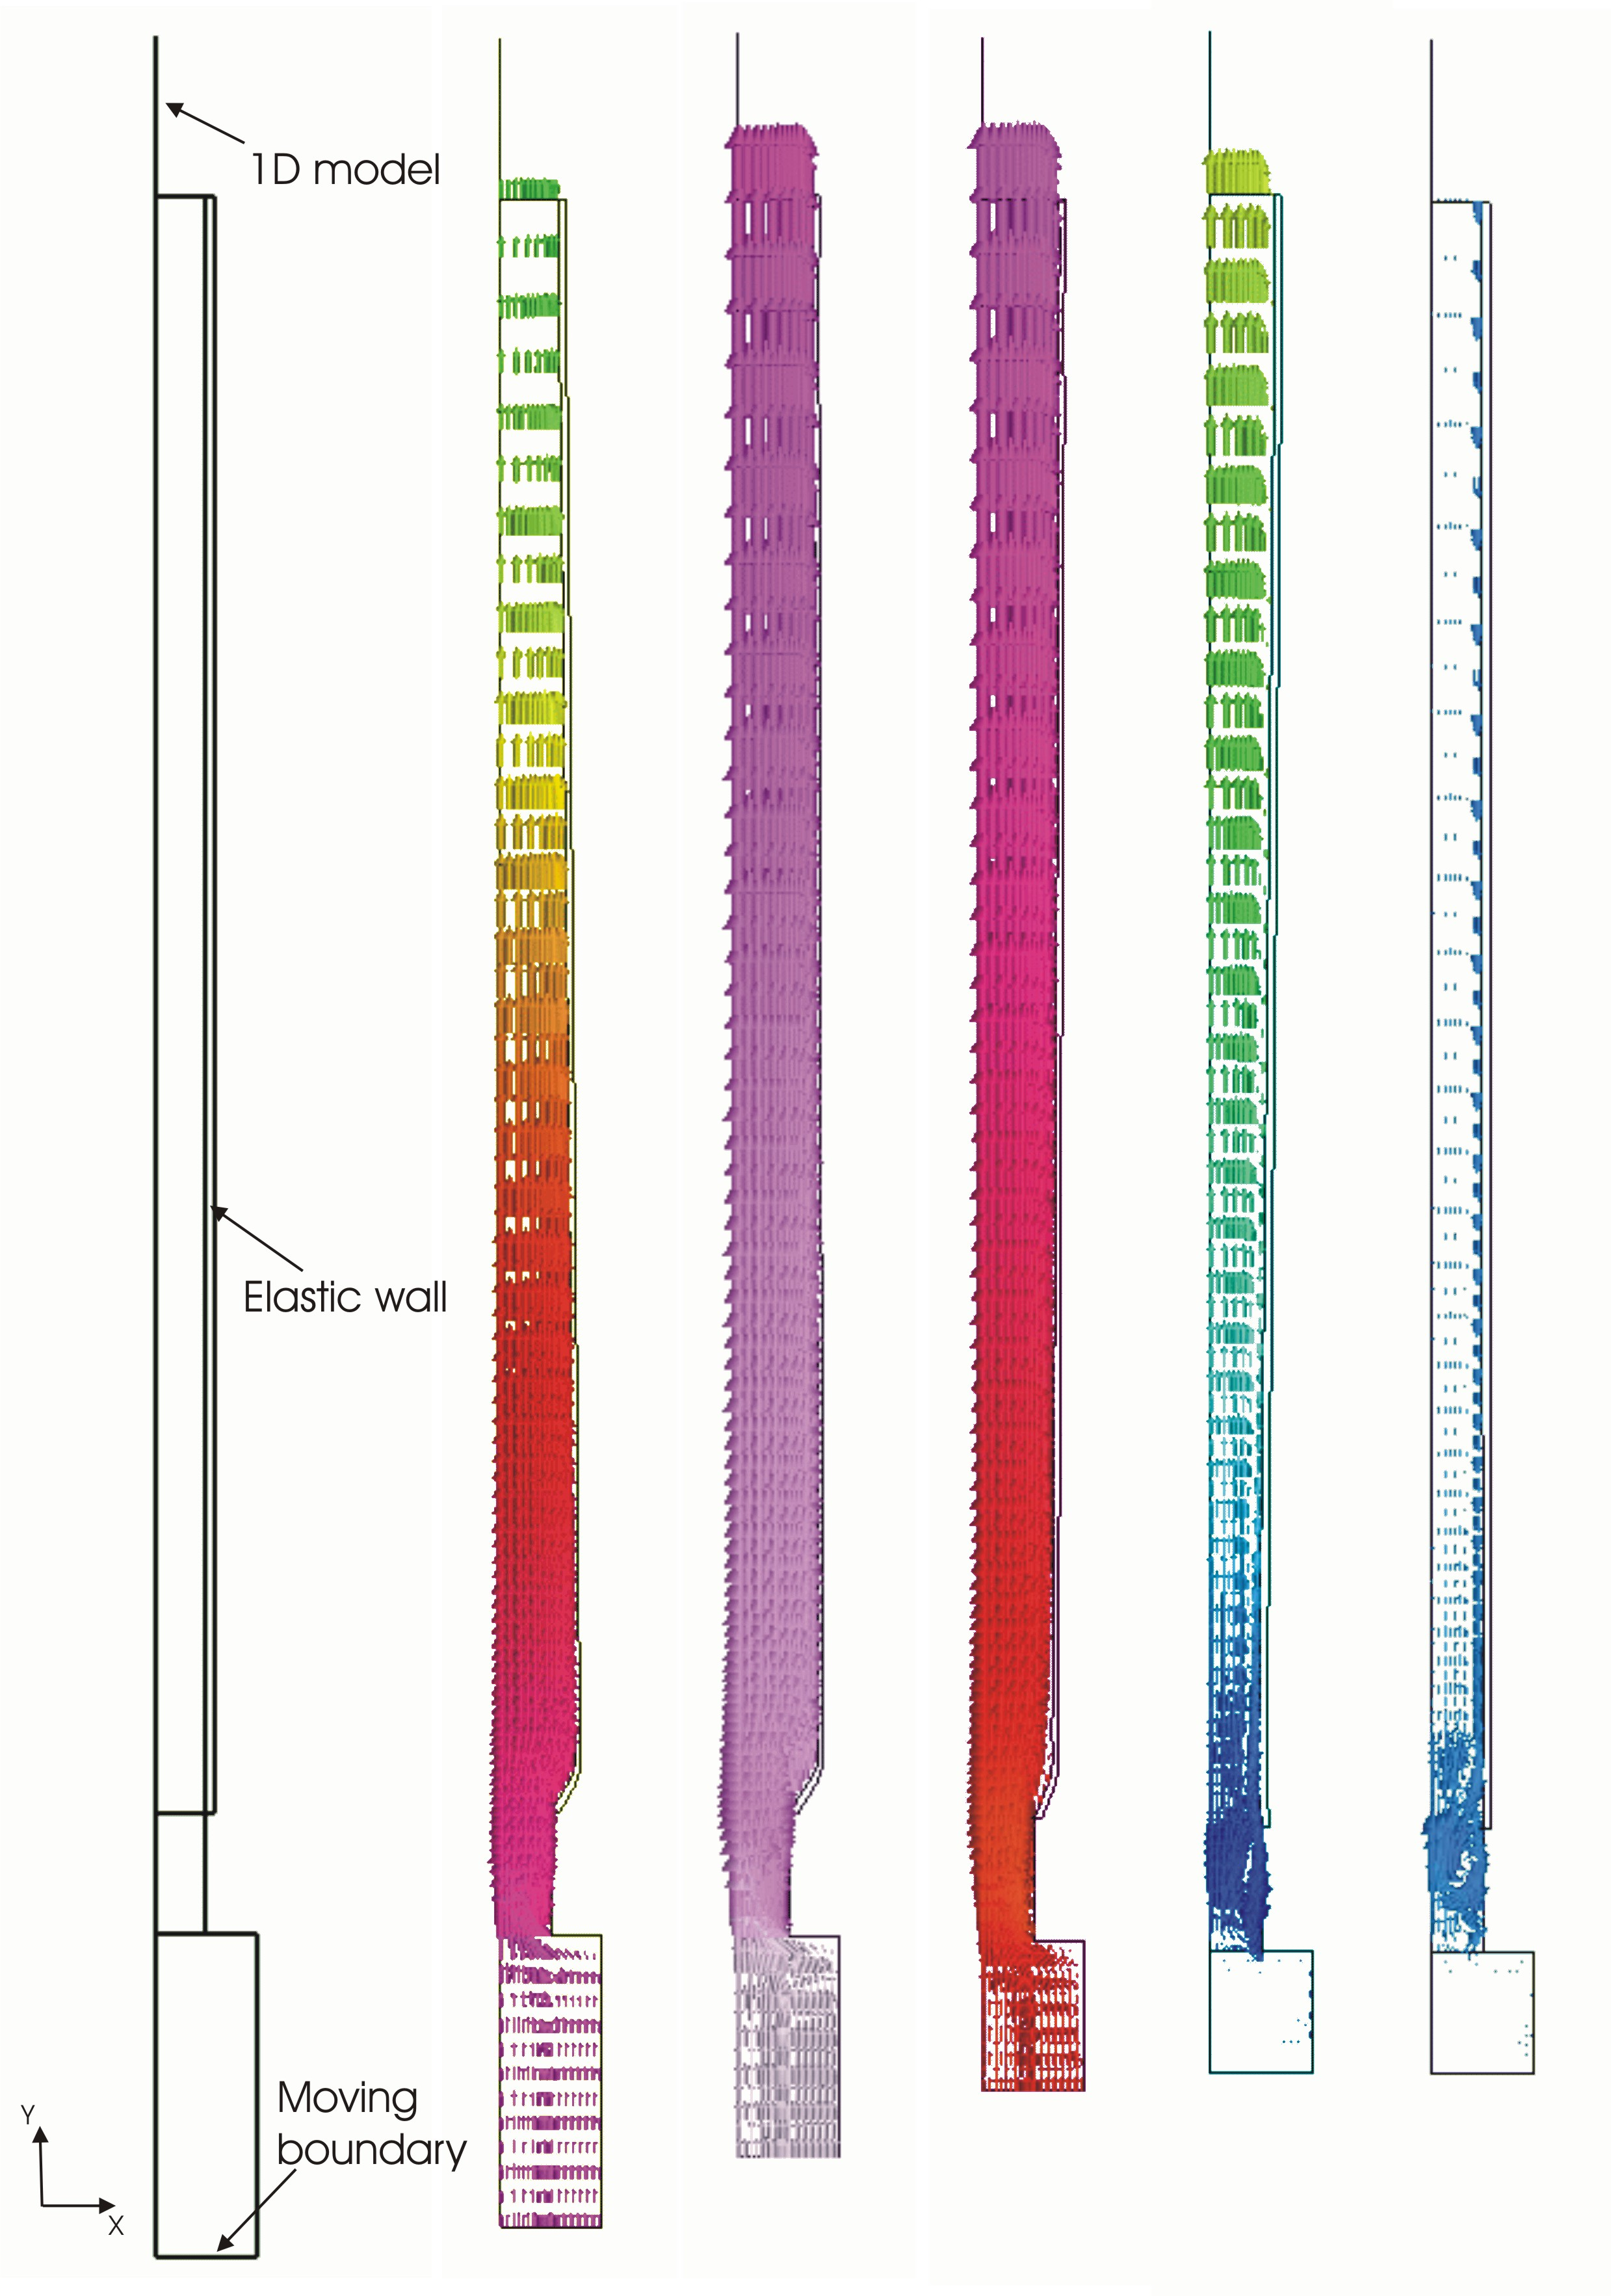
\includegraphics[width=\textwidth]{collage}
\caption{The geometry of the model and velocity fields at 5 time steps, 
100, 200, 300, 400 and 500 ms.  The displacements of the wall are 
magnified by factor of 10.}
\label{fig:velofields}
\end{center}
\end{figure}





%\part{Utility Problems}

%\graphicspath{{./}{TemperatureOperatorSplitting/}}
%\chapter{Operator splitting in the evolutionary heat equation}

\modinfo{Directory}{TemperatureOperatorSplitting}
\modinfo{Solvers}{HeatSolve, TransportEquationSolver, 
RateOfChangeSolver} 
\modinfo{Tools}{Editor} 
\modinfo{Dimensions}{2D, Transient simulation}


\subsection*{Introduction}

The drawback of the stabilized finite element formulations available
in Elmer to solve the convection-diffusion equation and Navier-Stokes
equations is that these methods are computationally expensive, in particular
when the residual-free-bubbles formulation is used.
In evolutionary problems the reduction of computational cost may be attempted
by applying operator splitting techniques in which the original equation at
each time step is split up into subproblems that are
easier to solve numerically.

The aim of this chapter is to provide an illustrative example on
using operator splitting capability in the solution of the 
time-dependent heat equation. 
% and Navier-Stokes equations.   
For the theoretical background of the operator splitting scheme applied here
the reader is referred to Elmer Models Manual and references therein.


%\section{Example I: The evolutionary heat equation}

\subsection*{Case description}

The problem considered here is the solution of the time-dependent 
heat equation in the homogeneous L-shaped plate the geometry of which is shown 
in Figure~\ref{fg:struct1}. 
The density of the material is taken to be unity, while the heat 
conductivity $k$ of the material is taken to be a 
parameter with values ranging between 0.05 and 0.01. The plate is
heated by a constant internal heat source magnitude of which equals to unity. 
The convection velocity field is assumed to be constant with the two 
Cartesian components of the velocity vector equaling to unity. 
The boundaries $\Gamma_i$,
$i=1,4,5,6$, are kept at constant temperature $0$, while the boundaries
$\Gamma_2$ and $\Gamma_3$ are assumed to be insulated, i.e.\ the heat flux
on this part of the boundary vanishes. 

The problem is to solve the temperature distribution in the plate. 
The time interval for the simulation is taken to be [0,2] and the temperature 
of the plate is 0 at the time $t=0$. 


\subsection*{Solution procedure}

Using operator splitting the solution of the heat equation may be replaced 
at each time step by the solution of three subproblems consisting of two 
time-dependent Poisson equations and the convective transport problem.
The effects of diffusion and convection are decoupled by this 
splitting so that 
the diffusion and convection phenomena are taken into account by the steps 
involving the solution of the Poisson equation and the convective transport 
problem, respectively. 

The time-dependent Poisson equations can be solved using the basic heat 
equation solver in Elmer. To avoid the use of stabilized finite element 
formulations in the solution of the convective transport problem this 
subproblem is solved by discretizating an equivalent wave-like equation 
formulation (second order in time equation). 
  
When the operator splitting method is applied,
specific care is needed in prescribing boundary and initial conditions
for the simulation. While the boundary conditions (and initial conditions) 
for the steps involving the solution of the Poisson equation may be defined in 
the usual manner, the boundary conditions for the convective 
transport problem may be prescribed
only on the part of inflow boundary on which the temperature is prescribed. 
In the example the inflow boundary is the union of the boundary segments 
$\Gamma_i$, $i=1,2,5,6$,
so the boundary conditions for the convective transport equation 
should be given on $\Gamma_i$, $i=1,5,6$.
In addition to prescribing the boundary conditions, the rate of change of
the field subject to the convection operator (here temperature) is needed as 
an initial condition at the beginning of pure convection step. This field 
can be solved using a specific solver ({\tt RateOfChangeSolver}) prior to
the solution of the convective transport problem. 
The boundary conditions for this 
solver should be prescribed on the same part of the boundary on which the 
boundary conditions for the convective transport problem are prescribed.    

It should be noted that in connection with the operator splitting method
the user should specify an even number of time steps.
Although the details of implementation need not be known in order to use
the operator splitting ability, it is noted that the the running of two 
successive time steps actually constitutes a single operator splitting scheme
step as described in Elmer Models Manual. 
There are thus three equations (referred to as {\tt Heat Equation},
{\tt Rate Of Change Equation} and {\tt Transport Equation}) which may be 
solved at one time step. 
At odd time steps all these equations are solved meaning that
both the diffusion and convection steps are taken, whereas at even time
steps the solution of the convective transport problem is omitted so that
the diffusion step is performed only. Physically meaningful results
satisfying all the essential boundary conditions may thus be written to
the results file only after even time steps.
 
The mesh for this example was created using Femlab and tools for 
converting meshes from Femlab to Elmer format. The mesh in Elmer format is 
given in the tutorial files. This unstructured mesh
consists of 8458 elements each of which having three nodes.    

The Header section of the solver input file is used to declare the directory
containing the Elmer mesh files:

\ttbegin
Header
  Mesh DB "." "femlab-mesh"
End
\ttend

The Simulation section of the solver input file is used to declare the 
coordinate system and simulation type as well as simulation parameters 
related to the time discretization scheme: 

\ttbegin
Simulation
  Coordinate System = String "Cartesian 2D"
  Simulation Type = String "Transient"
  Timestepping Method = String "Crank-Nicolson"
  Timestep Intervals(1) = Integer 200
  Timestep Sizes(1) = Real 0.01
  Output Intervals(1) = Integer 1
  Steady State Max Iterations = Integer 1
  Post File = File "os-example.ep"
End
\ttend

Here the keyword {\tt Timestepping Method} is used to 
define the time discretization scheme that is used in the solution of the 
time-dependent Poisson equations. Note that one should not use 
multi-step methods in connection with the operator splitting method. 
The time discretization scheme that is used
in the solution of the convective transport problem is fixed and need not
be specified. It should be noted also that
the number of time steps should be even. Since the equations
solved at one time step are not coupled and can thus be solved in sequential 
manner, {\tt Steady State Max Iterations} may be taken to be 1.     

The Body section of the solver input file is used to declare integer 
identifiers for body forces, equations, initial conditions and materials: 

\ttbegin
Body 1
  Body Force = Integer 1
  Equation = Integer 1
  Initial Condition = Integer 1
  Material = Integer 1
End
\ttend

The Equation section of the solver input file in turn has the following 
declaration

\ttbegin
Equation 1
  Active Solvers(3) = Integer 1 2 3
End
\ttend
indicating that three equations are to be solved using solvers with 
the integer identifiers 1, 2 and 3.   
Accordingly, three Solver sections are needed.  
The first Solver section is used for the Poisson equation and has the 
following declarations:

\ttbegin
Solver 1
  Equation = String "Heat Equation"
  Variable = String "Temperature"
  Variable Dofs = Integer 1
  Linear System Solver = String "Iterative"
  Linear System Iterative Method = String "BiCGStab"
  Linear System Max Iterations = Integer 350
  Linear System Convergence Tolerance = Real 1.0e-08
  Linear System Abort Not Converged = Logical True
  Linear System Preconditioning = String "ILU0"
  Steady State Convergence Tolerance = Real 1.0e-05
  Stabilize = Logical False
  Bubbles = Logical False
End
\ttend
Note that there is no need to use stabilization, so the values of the keywords 
{\tt Stabilize} and {\tt Bubbles} may be set to be {\tt False} to reduce the
computational cost. 

The remaining two Solver sections are related to the convective transport
problem. The first one of these sections is used to declare the solver
parameters related to the problem ({\tt Rate Of Change Equation}) the 
solution of which gives the approximation to the rate of change of the 
temperature at the beginning of pure convection step. The contents
of this solver section is 

\ttbegin
Solver 2
  Equation = String "Rate Of Change Equation"
  Procedure = File "RateOfChange" "RateOfChangeSolver"
  Variable = String "Udot0"
  Variable Dofs = Integer 1   
  Advection = String "Constant"
  Advection Variable = String "Temperature" 
  Linear System Solver = String "Iterative"
  Linear System Iterative Method = String "BiCGStab"
  Linear System Max Iterations = Integer 350
  Linear System Convergence Tolerance = Real 1.0e-08
  Linear System Abort Not Converged = Logical True
  Linear System Preconditioning = String "ILU0"
  Steady State Convergence Tolerance = Real 1.0e-05
End
\ttend

Here the keyword {\tt Advection Variable} is used to declare the quantity
which is subject to the convection operator, while the keyword {\tt Advection}
is used to define the type of the velocity vector.
The name {\tt Udot0} is used for the solution of this problem.

Finally, the Solver section for the wave-like equation, which is equivalent to 
the convective transport equation, has the following declarations:

\ttbegin
Solver 3  
  Equation = String "Transport Equation"
  Procedure = File "TransportEquation" "TransportEquationSolver"
  Time Derivative Order = Integer 2
  Variable = String "U"
  Variable Dofs = Integer 1  
  Advection = String "Constant"
  Advection Variable = String "Temperature" 
  Rate Of Change Equation Variable = String "Udot0" 
  Linear System Solver = String "Iterative"
  Linear System Iterative Method = String "BiCGStab"
  Linear System Max Iterations = Integer 350
  Linear System Convergence Tolerance = Real 1.0e-8
  Linear System Abort Not Converged = Logical True
  Linear System Preconditioning = String "ILU0"
  Steady State Convergence Tolerance = Real 1.0e-05
End
\ttend

The name {\tt U} is used for the solution of the convective transport problem. 
The value of the keyword {\tt Time Derivative Order} must be 2.
The use of the keywords {\tt Advection Variable} and {\tt Advection}
is similar to that explained in connection with the second solver section.  

The Material section is used to declare the material properties and,
as the velocity vector in the convection operator is of constant type,
also the components of the velocity vector. In the case $k=0.01$ the contents 
of this section is  

\ttbegin
Material 1
  Density = Real 1
  Heat Capacity = Real 1
  Heat Conductivity = Real 0.01
  Advection Velocity 1 = Real 1
  Advection Velocity 2 = Real 1
End
\ttend

Body Force section is used to declare the body force in the Poisson
equations.

\ttbegin
Body Force 1
  Heat Source = Real 1
End
\ttend

Finally, the initial conditions and boundary conditions are specified. 
The temperature at $t=0$ is defined by giving the declaration  

\ttbegin
Initial Condition 1
  Temperature = Real 0
End
\ttend

Two Boundary Condition sections are needed. The first one is used 
to prescribe the boundary conditions on the part of inflow boundary where
the temperature is given: 

\ttbegin
Boundary Condition 1
  Target Boundaries(3) = Integer 1 2 4 
  Temperature = Real 0
  Udot0 1 = Real 0
  U 1 = Real 0
End
\ttend

The rate of change of the temperature is zero on this part of the boundary 
as the temperature is kept fixed. Thus the zero boundary 
conditions for {\tt Udot0} are defined. The boundary value of the 
solution to the convective transport problem should equal to the
temperature. Therefore zero boundary conditions for {\tt U} are also defined.
  
The second Boundary Condition section is used to define the Dirichlet boundary 
conditions on the outflow boundary: 

\ttbegin
Boundary Condition 2
  Target Boundaries(1) = Integer 3
  Temperature = Real 0
End
\ttend

Note that the zero heat flux condition
need not be specified explicitly. Similarly, the treatment of 
the outflow boundary conditions for the wave-like
equation are handled automatically by the code and need not be specified. 


\subsection*{Results}

From a numerical point of view the solution of the problem becomes 
increasingly difficult as the heat conductivity $k$ tends to zero. 
In order to examine possible dependence on the heat conductivity parameter
the problem was solved in three cases with $k$ taking values 0.05, 0.025 
and 0.01. For comparison the same case was solved using three alternative 
methods. Here the operator splitting scheme is referred to as OS, S is the 
stabilized finite element method and RFB is the method based on the 
residual-free-bubbles formulation. In the case of methods S and RFB the 
simulation was performed using 100 time steps which corresponds to the number 
of 200 time steps used in the case of operator splitting scheme.
 
The maximum temperature at $t=2.0$ is recorded in 
Table~\ref{methodvstemperature}. The CPU time used in the simulation to
obtain solution for a certain value of the heat conductivity is
shown in Table~\ref{methodvscpu}.
   
\begin{table}  
\caption{The maximum temperature at $t=2.0$. For comparison 
the maximum temperature according to the steady state solution is also 
recorded.}
\label{methodvstemperature}
\begin{center}
\begin{tabular}{lccc}\hline
Method            &        &  $k$   &                \\ \hline
                  & 0.05   & 0.025  & 0.01           \\ \hline
OS                & 1.0235 & 1.0424 & 1.0677         \\
S                 & 1.0269 & 1.0436 & 1.0418         \\
S(steady state)   & 1.0279 & 1.0437 & 1.0418         \\
RFB               & 1.0271 & 1.0458 & 1.0853         \\
RFB(steady state) & 1.0286 & 1.0462 & 1.1050         \\ \hline
\end{tabular}
\end{center}
\end{table}

\begin{table} 
\caption{CPU time used by the different methods for simulation ($k=0.01$).}
\label{methodvscpu}
\begin{center}
\begin{tabular}{lc}\hline
Method            & CPU     \\ \hline
OS                & 211.13  \\
S                 & 82.16   \\
RFB               & 340.70  \\ \hline
\end{tabular}
\end{center}
\end{table}


\subsection*{Discussion}

The benefit of the wave-like equation formulation of the convective 
transport problem is that this formulation can be discretized without
using stabilized finite element formulations. Thus all the subproblems
arising from operator splitting can be solved using standard FE
techniques. On the other hand,
the expense of this approach is that one is lead to handle the second
order in time equation. 

In the current implementation of the method the 
wave-like equation is discretized in time
using the Crank-Nicolson scheme which is expected to perform well if 
the solution to the convective transport problem is smooth. Spurious
oscillations may however occur in the case of a rough solution changing 
rapidly in short length scales. The user of the method should be
aware that the deterioration of accuracy may thus occur if the solution is
not smooth and $\epsilon=k/||\vec u ||_\infty \longrightarrow 0$,
meaning that convection dominates.  
   
In the cases considered convection dominates, the parameter $\epsilon$ 
ranging between $3.5\cdot 10^{-2}$ and $7.1\cdot 10^{-3}$,
and the solution has also sharp boundary 
layer near the upper edge. No spurious oscillations are however detected in
the solution. Nevertheless, the results recorded in 
Table~\ref{methodvstemperature} indicate that the differences between the
methods become larger as $\epsilon \longrightarrow 0$. 
 
In view of the results shown in Table~\ref{methodvscpu} the accuracy of the 
operator splitting scheme in predicting the maximum temperature is comparable 
to that of the residual-free-bubbles method while the computational 
cost measured in CPU time is reduced by approximately 40~\% when 
the operator splitting scheme is used. 

It should be noted that the operator splitting scheme has 
the favourable feature that small spurious oscillations present in the 
solution after pure convection step may naturally be damped by the step 
involving diffusion phenomena. Note also that each of the subproblems arising 
from the operator splitting may be
solved very efficiently using multigrid techniques, whereas robust multigrid 
solvers amenable to solving linear systems arising from direct discretization 
of the convection-diffusion equation are still to be found. This makes 
the operator splitting scheme attractive in the solution of problems 
having a very large number of unknowns.   




%\section{Example II: The evolutionary Navier-Stokes equations}





\graphicspath{{./}{PoissonBEM/}}
\chapter{Temperature distribution with BEM}

\modinfo{Directory}{PoissonBEM}
\modinfo{Solvers}{\Idx{PoissonBEMSolver}}
\modinfo{Tools}{\Idx{ElmerGrid}, editor}
\modinfo{Dimensions}{2D}

\subsection*{Case definition}
This tutorial uses boundary element method (\Idx{BEM}) to solve Poisson equation.
Even though Elmer is primarily a finite element software the are limited
support also for BEM computation. One should however note that Elmer does not
include any multilevel strategies essential for a good performance.
For more details about BEM check the Elmer Models Manual.
The simulation setting is described in Figure~\ref{f:simulationSetting}. 
A heater with constant heat flux is placed inside a box and the walls of the box are in 
fixed temperature.
We are interested in the temperature distribution in the medium around the heater ($\Omega$)
and on the surface of the heater ($\Gamma_1$). We also want to know the heat flux through the
walls of the box ($\Gamma_2$).
\begin{figure}[!htb]
\begin{center}
\setlength{\unitlength}{0.17cm}
\begin{picture}(30,30)
% box walls  *****************
\put(0,0){\line(1,0){30}}
\put(0,30){\line(1,0){30}}
\put(0,0){\line(0,1){30}}
\put(30,0){\line(0,1){30}}
% heater walls ***************
\put(10,10){\line(1,0){10}}
\put(10,20){\line(1,0){10}}
\put(10,10){\line(0,1){10}}
\put(20,10){\line(0,1){10}}
% some text ******************
\put(11,25){$\Omega$, medium}
\put(12.5,14.5){heater}
\put(10,7.5){$\Gamma_1$, $-\frac{\partial T}{\partial n} = 1$}
\put(11,1){$\Gamma_2$, $T=0$}
\end{picture}
\end{center}
\caption{Simulation setting}
\label{f:simulationSetting}
\end{figure}

\subsection*{Solution Procedure}
First we create a mesh with ElmerGrid. The mesh is defined in
{\tt heater.grd} and it is created with command
\ttbegin
ElmerGrid 1 2 heater
\ttend
The solver input file {\tt PoissonBEM.sif} starts with 
the definition of the mesh directory. 
\ttbegin
Header
  Mesh DB "." "heater"
End
\ttend
The simulation uses 2D Cartesian geometry, searches a steady state and since
there is no coupled solvers only one iteration is needed.
Numerical results for restart are written to file {\tt BEM\_Temperature.result}
and file for Paraview visualization is {\tt BEM\_Temperature.vtu}.
\ttbegin
Simulation
  Coordinate System =  Cartesian 2D
  Coordinate Mapping(3) = 1 2 3

  Simulation Type = Steady
  Steady State Max Iterations = 1

  Output Intervals = 1
  Post File = "BEM_Temperature.vtu"
  Output File = "BEM_Temperature.result"
End
\ttend
There is just one body, the medium around the heater, and it uses equation 1.
\ttbegin
Body 1
  Name = "medium"
  Equation = 1
End
\ttend
In equation block we say that we use the solver named {\tt PoissonBEM}.
\ttbegin
Equation 1
  PoissonBEM = Logical True
End
\ttend
In solver block the {\tt Equation} keyword must match the one in equation block.
We also need to define the procedure, name the variable ({\tt Temperature}) and tell 
the degrees of freedom of the variable. Keyword {\tt Optimize Bandwidth} must be set to false
with BEM solver. Since we were interested in the flux, we must now export it to the
results. The lines beginning {\tt Exported} must be exactly as below. Keywords beginning
{\tt Linear System} can be used except that the preconditioning cannot be ILU.
\ttbegin
Solver 1
  Equation = PoissonBEM
  Procedure = "PoissonBEM" "PoissonBEMSolver"
  Variable = Temperature
  Variable DOFs = 1

  Optimize Bandwidth = False

  Exported Variable 1 = String Flux
  Exported Variable 1 DOFs = 1

  Linear System Solver = Iterative
  Linear System Iterative Method = BiCGStab
  Linear System Preconditioning = Jacobi
  Linear System Max Iterations = 100
  Linear System Convergence Tolerance = 1.0e-8

  Steady State Convergence Tolerance = 1.0e-6
End
\ttend
Finally we give the boundary conditions for the heater surface and for the walls of the 
box. The keyword {\tt Body Id} tells the reference body of this boundary. Here it is 1. 
The keyword {\tt Normal Target Body} tells the direction of the outer normal. Value -1 
means the side where there are no volume elements. We didn't mesh the inside of 
the heater and so we can use value -1 in both cases. The heat flux from heater to
medium is 1 and the walls of the box are set to zero temperature. The keyword
{\tt Temperature} matches the name of the variable in solver block.
\ttbegin
Boundary Condition 1
  Name = "heater_surface"
  Target Boundaries = 1

  Body Id = 1
  Normal Target Body = Integer -1
  Flux = Real 1
End

Boundary Condition 2
  Name = "box_walls"
  Target Boundaries = 2

  Body Id = 1
  Normal Target Body = Integer -1
  Temperature = 0
End
\ttend
\subsection*{Results}
Problem is solved with command {\tt Solver}. The results are here viewed with
{\tt ElmerPost}. In Figure~\ref{f:temperature} is the temperature distribution.
\begin{figure}[!hb]
\begin{center}
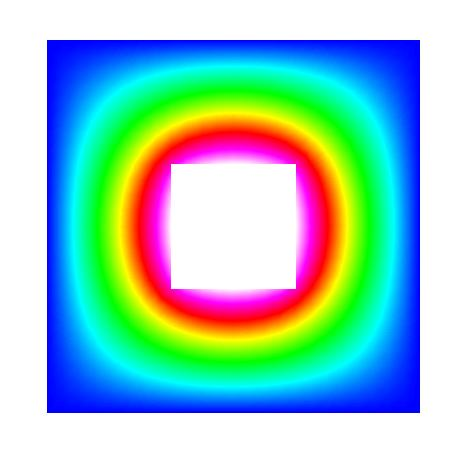
\includegraphics[width=0.4\textwidth]{temperature}
\end{center}
\caption{The temperature distribution.}
\label{f:temperature}
\end{figure}





















\graphicspath{{./}{Temperature1D/}}
\chapter{Adding user defined equation solver}

\modinfo{Directory}{Temperature1D}
\modinfo{Solvers}{\Idx{PoissonSolver}} 
%\modinfo{Files}{1dheat.grd, 1dheat.sif, Poisson.f90}
\modinfo{Tools}{Editor, \Idx{Fortran 90 compiler}, \Idx{ElmerGrid}}
\modinfo{Dimensions}{1D, Steady-state}

\subsection*{Problem description}

This tutorial is about creating the code for a simple poisson equation solver.
The solver is applied to 1d case with internal source term and fixed boundaries.

Mathematically the problem we solve is
\begin{equation}
\left \{
\begin{array}{cccc}
- \Delta \Phi &= &f & \mbox{ in } \Omega \\
\Phi&=&0 & \mbox{ on } \Gamma
\end{array}
\right .
\end{equation}

Allthough this example is in 1d the same solver code also applies to 2D and 3D
problems.

\subsection*{Solution procedure}

Custom Fortran 90 code solving some specific equation may be added dynamically to Elmer 
software. Here we create a very simple equation solver code. The final code
may be found in the tutorial directory as well as the files for running
the example. The solution may be attempted as follows:

\begin{itemize}
\item Copy all the files from tutorial directory to current directory
\item Setup Elmer
\item Give the following commands:
\ttbegin
elmerf90 -o Poisson Poisson.f90
ElmerGrid 1 2 1dheat
ElmerSolver
ElmerPost
\ttend
\end{itemize}

\subsection*{The solver code}

The example Fortran code may be found in the tutorial files under the
name Poisson.f90.  The example run is defined in 1dheat.sif.
Only a rough guideline is given here of both of the files, refer to the
files themselves for more details.

All the  equation solvers in Elmer have the following common interface
\ttbegin
SUBROUTINE PoissonSolver( Model, Solver, dt, TransientSimulation )
  USE SolverUtils

  TYPE(Model) :: Model
  TYPE(Solver_t), POINTER :: Solver
  REAL(KIND=dp) :: dt
  LOGICAL :: TransientSimulation

    ...
END SUBROUTINE PoissonSolver
\ttend

The argument Model contains pointers to the whole definition of the Elmer run.
The argument Solver contains parameters specific to our equation solver.
The argument dt and TransientSimulation are the current time step size, and a
flag if this run is steady or transient. These don't concern us this time.

When starting the ElmerSolver looks in solver input (.sif) file for a
Solver section with keyword "Procedure". This should contain reference to
the compiled code

\ttbegin
   Procedure = "Poisson" "PoissonSolver"
\ttend
where the first string in the right hand side is the file name of the compiled
code, and second argument is the name of the subroutine to look for in the given file.

In the Solver section one also gives the name of the field variable
(here Poisson) and the DOFs/node (here 1).

The basic duty of the equation solver is to solve one or more field variables inside
the time progressing- or steady state iteration-loop of ElmerSolver.  Here we use
FEM to discretize the Poisson equation and finally solve the equation by calling
ElmerSolver utility SolveSystem.

The solution progresses the following way:

\begin{itemize}
\item Get the space for variables and temporaries from ElmerSolver and compiler.
The matrix structure and space for solution and RHS vector have already been
allocated for you before you enter the equation solver.

The matrix is of type Matrix\_t and may be obtained from the arguments as
\ttbegin
TYPE(Matrix_t), POINTER :: StiffMatrix
StiffMatrix => Solver % Matrix
\ttend
Usually one doesn't need to know the internal storage scheme or the fields
of the Matrix type, but one just passes this pointer further to ElmerSolver
utility routines.

Similarly, the force vector may be accessed as follows:
\ttbegin
REAL(KIND=dp), POINTER :: ForceVector(:)
ForceVector => StiffMatrix % RHS
\ttend

The solution vector is obtainable similarly
\ttbegin
TYPE(Variable_t), POINTER :: Solution
Solution => Solver % Variable
\ttend

The Variable\_t structure contains the following fields
\begin{itemize}
\item DOFs: the number of degrees of freedom for one node. This value is for
information only and shouldn't be modified.
\item Perm: an integer array that is non-zero for nodes that belong
to computational volume for this equation. The entry $Perm(i)$ holds
the index of the global matrix row  (for 1 DOF) for nodal point i.
This array  shouldn't be modified by the equation solver.
\item Values: Space for the solution vector values.
Note that the values
are ordered the same way as the matrix rows, .i.e. the value of Potential at node
n is stored at
\ttbegin
  val = Solution % Values( Solution % Perm(n) )
\ttend
\end{itemize}


\item Initialize the global system to zero. Calling the utility routine
\ttbegin
CALL InitializeToZero( StiffMatrix, ForceVector )
\ttend
is usually enough.


\item Go through the elements for which this equation is to 
be solved, get the elemental matrices and vectors and add them to
the global system:

\ttbegin
DO i=1,Solver % NumberOfActiveElements
   CurrentElement => Solver % Mesh % Elements( Solver % ActiveElements(i) )
      ...
   CALL LocalMatrix( ... )
   CALL UpdateGlobalEquations( ... )
END DO
CALL FinishAssembly( ... )
\ttend

Here the LocalMatrix is your own subroutine computing elemental matrices and vectors.
In the example code LocalMatrix uses three routines from ElmerSolver utilities. The function 
\ttbegin
  dim = CoordinateSystemDimension()
\ttend
returns the dimension of the current coordinate system, i.e. the return value is 
1, 2 or 3 depending on the input file setting of keyword "Coordinate System". The function
GaussPoints returns structure containing the integration point local coordinates and weights
\ttbegin
  TYPE(GaussIntegrationPoints_t) :: IntegStuff
  IntegStuff = GaussPoints( Element )
\ttend
The fields of the type GaussIntegrationPoints\_t are
\ttbegin
INTEGER :: n
REAL(KIND=dp) :: u(:), v(:), w(:), s(:)
\ttend
the integer value n is the number of points selected. The arrays u,v and w
are the local coordinates of the points, and the array s contains the weights
of the points. One may call the GaussPoints-routine with second argument,
\ttbegin
  IntegStuff = GaussPoints( Element, n )
\ttend
if the default number of integration points for given element is not suitable.

Inside the integration loop the function ElementInfo is called:
\ttbegin
   TYPE(Element_t), POINTER :: Element
   TYPE(Nodes_t) :: Nodes
   REAL(KIND=dp) :: U,V,W,detJ, Basis(n), dBasisdx(n,3), ddBasisddx(n,3,3)

   stat = ElementInfo( Element, Nodes, U, V, W, detJ,  &
        Basis, dBasisdx, ddBasisddx, .FALSE. )
\ttend
This routine returns determinant of the element jacobian (detJ), basis function values
(Basis(n)), basis function global derivative values (dBasisdx(n,3)), basis function second
derivative values ( ddBasisddx(n,3,3) ). The second derivatives are only computed if the
next logical flag is set to true. All the values are computed at the point U,V,W inside
element defined by structures Element and Nodes.

Refer to the code for more details.

\item Set boundary conditions. Here only dirichlet boundary conditions are used. These
may be set by using the utility routine SetDirichletBoundaries.

\item Solve the system by calling utility routine SolveSystem.
\end{itemize}


\begin{figure}
\begin{center}
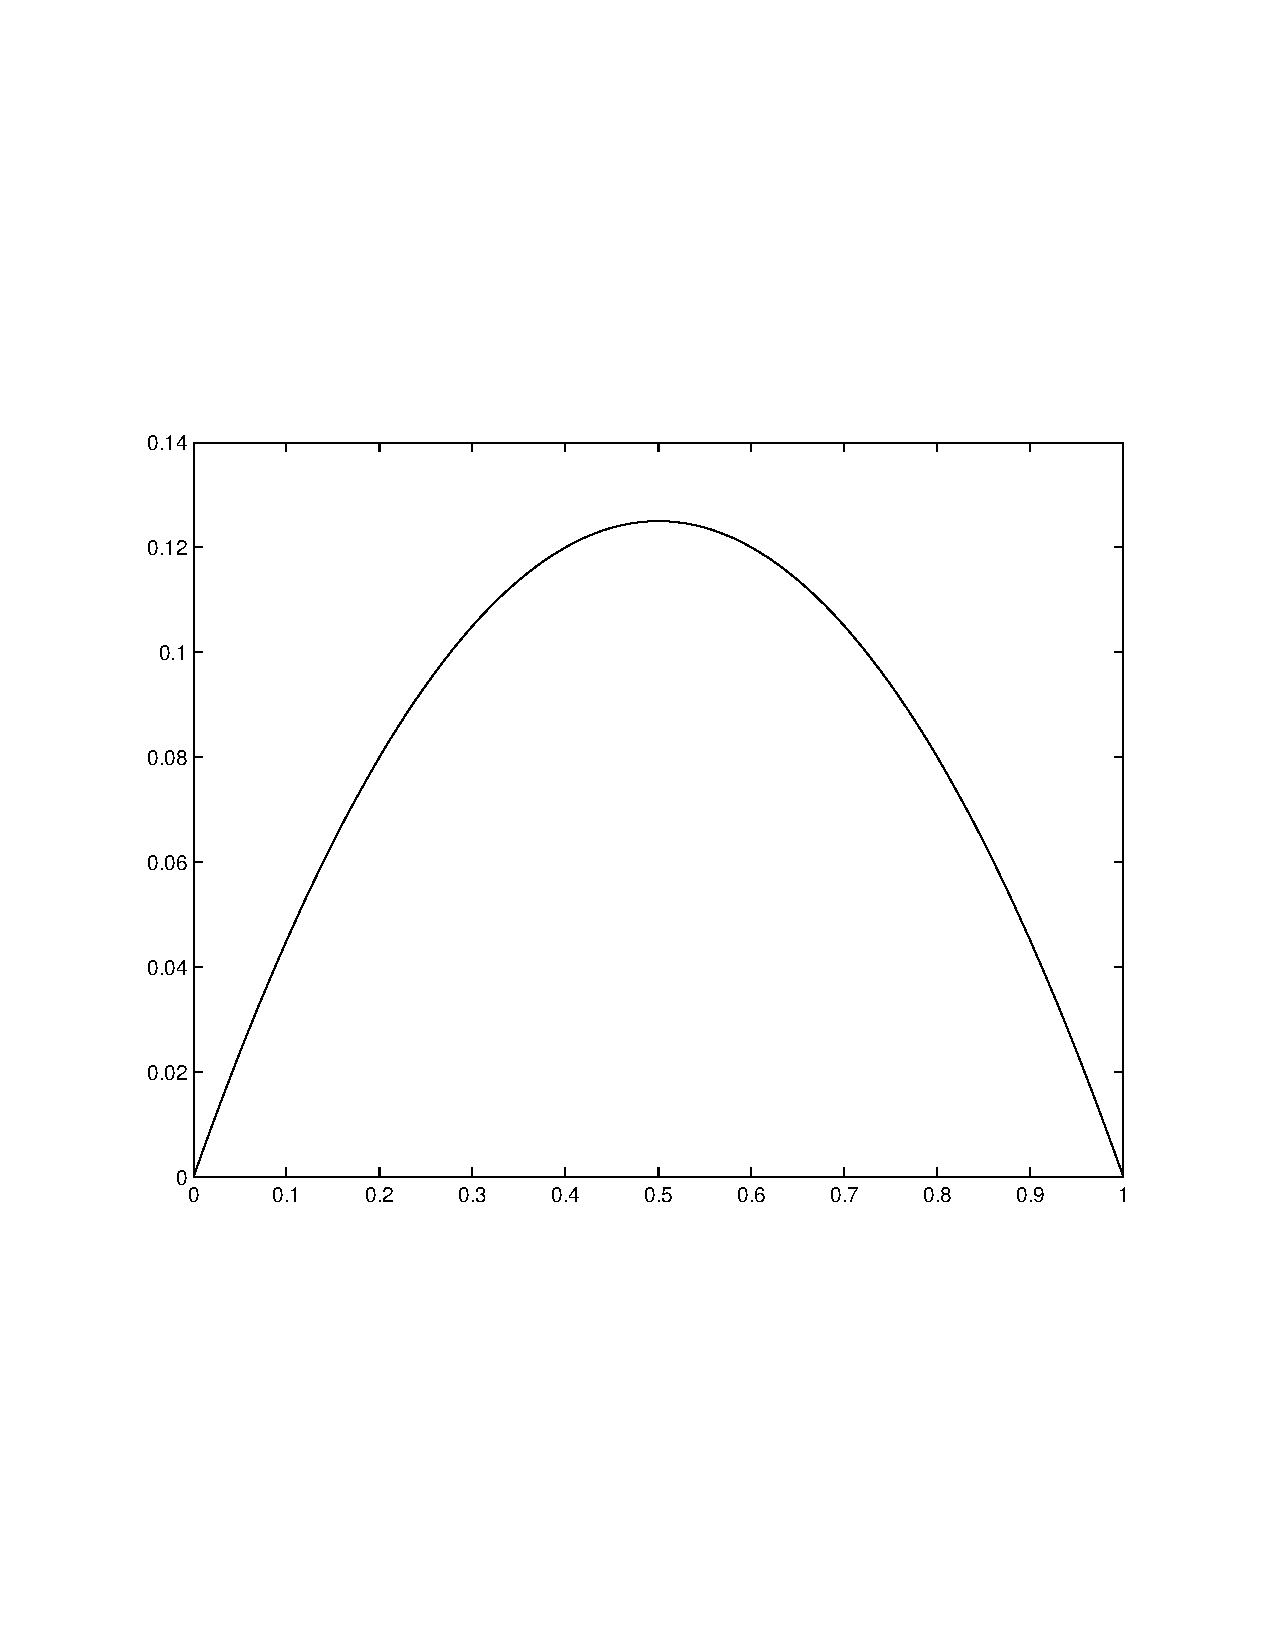
\includegraphics[width=0.6\textwidth]{1dheat}
\caption{Solution of the Poisson Equation.}\label{fg:pot}
\end{center}
\end{figure}
\subsection*{Results}

In the elmerpost file there is a variable called Potential which contains the
solution of this simple example. See figure~\ref{fg:pot}


\graphicspath{{./}{FlowLinearRestriction/}}
\chapter{Volume flow boundary condition}

\modinfo{Directory}{FlowLinearRestriction}
\modinfo{Solvers}{\Idx{FlowSolve}, \Idx{SolveWithLinearRestriction}} 
\modinfo{Tools}{Editor, \Idx{Fortran 90 compiler}, \Idx{ElmerGrid}}
\modinfo{Dimensions}{2D, Transient}

\subsection*{Case definition}

This tutorial gives an example how to use SolveWithLinearRestriction. It also describes
how to execute own functions before the original system is solved. In order to
understant the case reader should be familiar with \Idx{compressed row storage} matrixes and
elmer basics. This tutorial gives only the guidelines and reader is adviced to
read the files in order to get more through understanding.

We simulate the flow of incompressible fluid in a pipe.
The pipe has a length of 5 and a width of 1. On the left end we want to describe
a certain timedependent volume flow. In other words, we don't want to describe the velocity field
here but we want the velocity field be such that it transports certain amount of volume
in timeinterval. We could integrate the correct volume flow, but let's now approximate it
to make the more important aspects more visible. Our approximation here is that the volume
flow is proportional to average velocity on the edge i.e.
\begin{equation}
\frac{1}{N}\sum_{i=1}^{N}u_i = \frac{volume}{time}
\end{equation}
Here $u_i$ are the nodal velocities parallel to the pipe on the left edge and $N$ is the number of nodes on
the left edge. We want to set a nicely scaled sinusoidal volume flow on the edge, which leads to
\begin{equation}
\sum_{i=1}^{N}u_i = 10N\sin(2\Pi t)
\end{equation}
This equation we can (easily) force with lagrange multiplier.

\subsection*{Solution procedure}
First we make a uniform mesh of 800 four-node quadrilaterals with command
\ttbegin
ElmerGrid 1 2 mflow
\ttend
Next we construct the solver input file. Header is simply
\ttbegin
Header
  Mesh DB "." "mflow"
End
\ttend
The simulation block is also very simple. 
Here we need to define the timestepping method and timescale.
\ttbegin
Simulation
  Coordinate System = Cartesian 2D

  Simulation Type = Transient
  Steady State Max Iterations = 1

  Timestepping Method = BDF
  BDF Order = 1

  Timestep Sizes = 0.02
  Timestep Intervals = 100

  Output Intervals = 1

  Output File = "mflow.result"
  Post File = "mflow.ep"
End
\ttend
The body, material and equation blocks are as usual. The material parameters,
of course, have affect on the solution and interested reader is encouraged to
modify these values and recalculate the solution.
\ttbegin
Body 1
  Material = 1
  Equation = 1
End

Material 1
  Density = 3.0
  Viscosity = 0.1
End

Equation 1
  Navier-Stokes = TRUE
  Active Solvers(1) = 1
End
\ttend
The solver block has the usual Navier-Stokes keywords and two keywords
for volume flow boundary. 
The {\tt Before Linsolve} keyword defines binaryfile and function that is
called before the system is solved. This function we must write and
compile and we will come to it shortly. The following keyword,
{\tt Export Lagrange Multiplier}, states that we are not interested in 
the value of the Lagrenge multiplier and it is therefore not saved.
\ttbegin
Solver 1
  Equation = Navier-Stokes
  Stabilize = True

  Before Linsolve = "./AddMassFlow" "AddMassFlow"
  Export Lagrange Multiplier = Logical FALSE

  Linear System Solver = Iterative
  Linear System Iterative Method = BiCGStab
  Linear System Preconditioning = ILU1
  Linear System Max Iterations = 500
  Linear System Scaling = False
  Linear System Convergence Tolerance = 1.0e-8

  Nonlinear System Max Iterations = 15
  Nonlinear System Convergence Tolerance = 1.0e-8
  Nonlinear System Newton After Tolerance = 1.0e-4
  Nonlinear System Newton After Iterations = 8
  Nonlinear System Relaxation Factor = 1.0

  Steady State Convergence Tolerance = 1.0e-7
End
\ttend
In boundary conditions we state that both parallel and perpendiculer velocities
are zero on the pipe sides and on both edges the perpendicular velocity is zero.
Here we also define the number tags for the boundaries. The tag 2 is assigned to
boundary that has number 4 in grd-file, which is the left edge of the pipe.
To this tag number 2 we shall refer in our AddMassFlow-function.
\ttbegin
Boundary Condition 1
  Target Boundaries(2) = 1 3
  Velocity 1 = 0.0
  Velocity 2 = 0.0
End

Boundary Condition 2
  Target Boundaries = 4
  Velocity 2 = 0.0
End

Boundary Condition 3
  Target Boundaries = 2
  Velocity 2 = 0.0
End
\ttend
\subsection*{AddMassFlow function}
Here we shall only give some rough guidelines of the function, for more information
check the code. This function creates the constraint matrix and RHS that forces the
equation mentioned above. Then it calls SolveWithLinearRestriction to solve the system.
The coinstraint matrix is actually only a row-vector and the RHS is only one value. 
\begin{itemize}
\item The function parameters are defined in Elmer so you shouldn't change them.
\item First we set a pointer to EMatrix-field of the given system matrix.
If the pointed matrix is not yet allocated, calculate the number of nodes
on the edge we want to define the volume flow. This gives us the number of non-zeros
in our constraint matrix and we can allocate the matrix.
\item Set the rows, cols and diag -fields of the matrix. This sets the non-zeros
on their right places in the constraint matrix.
\item Set all values of the constraint matrix to unity.
\item Calculate the RHS-value. The current time was checked in the beginning 
of the function, so this is possible.
\item Call SolveWithLinearRestriction
\item Return 1 which tells the ElmerSolver that the system is already solved.
\end{itemize} 
The function is the compiled with command
\ttbegin
elmerf90 -o AddMassFlow AddMassFlow.f90 
\ttend
Here it is assumed that the source file name is AddMassFlow.f90.

\subsection*{Results}
Just say {\tt ElmerSolver} and you should get the solution in few minutes.
The velocity perpendicular to the pipe is practically zero and the velocity
parallel to the pipe is an example of \Idx{Womersley velocity profile}
\footnote{J.Physiol (1955) 127, 553-563}.
An interesting feature of this velocity profile is that on some timesteps 
the fluid flows to both directions, see figure~\ref{f:womersley}.
\begin{figure}[!hb]
\begin{center}
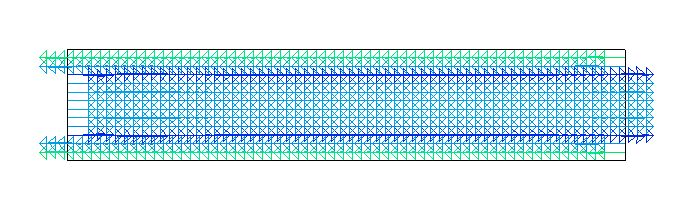
\includegraphics[width=\textwidth]{womersley}
\caption{Solution of the velocity field. Note the flow to both directions.}
\label{f:womersley}
\end{center}
\end{figure}



\graphicspath{{./}{FlowStreamlines/}}
\chapter{Streamlines}

\modinfo{Directory}{FlowStreamlines}
\modinfo{Solvers}{\Idx{StreamSolver}, \Idx{FlowSolve}}
\modinfo{Tools}{\Idx{ElmerGrid}, editor}
\modinfo{Dimensions}{2D}

\subsection*{Case definition}
The case definition is the same as in the incompressible flow passing a step.
The mathematical definition of the stream function $\psi$ is
\begin{equation}
u \, = \, \frac{\partial \psi}{\partial y} \, , \quad
v \, = \, - \frac{\partial \psi}{\partial x} \,.
\end{equation}
where $u,v$ are the velocity components in $x,y$ geometry.
For more info check Elmer Models Manual.

\subsection*{Solution Procedure}
First we create a mesh with ElmerGrid. The mesh is defined in
{\tt step.grd} and it is created with command
\ttbegin
ElmerGrid 1 2 step
\ttend
You may need to compile the StreamSolver yourself. If the Elmer environment is 
successfully setup the compilation command should look like
the following lines, 
\ttbegin
elmerf90 -o StreamSolver StreamSolver.f90
\ttend
The solver input file {\tt streamlines.sif} starts with 
the definition of the mesh directory. 
\ttbegin
Header
  Mesh DB "." "step"
End
\ttend
The simulation uses 2D Cartesian geometry and searches a Steady State.
There are no coupled solvers so only one iteration is needed. 
Numerical results are written to file {\tt streamlines.result}
and ElmerPost file is {\tt streamlines.ep}.
\ttbegin
Simulation
  Coordinate System =  Cartesian 2D
  Coordinate Mapping(3) = 1 2 3

  Simulation Type = Steady
  Steady State Max Iterations = 1

  Output Intervals = 1
  Post File = "streamlines.ep"
  Output File = "streamlines.result"
End
\ttend
There is just one body and it uses equation 1 and
is of material 1.
\ttbegin
Body 1
  Equation = 1
  Material = 1
End
\ttend
The equation block states that we use Solvers 1 and 2 to solve the problem
and that we use Navier-Stokes equations.
\ttbegin
Equation 1
  Active Solvers(2) = 1 2
  Navier-Stokes = True
End
\ttend
In material block we define the density and the viscosity of the fluid.
\ttbegin
Material 1
  Density = 1
  Viscosity = 0.01
End
\ttend
Solver 1 is for the Navier-Stokes equations.
Here we give the linear system solver
\footnote{Biconjugate gradient method with incomplete LU preconditioning}
and convergence criterions for linear, non-linear and steady state 
solution of the Navier-Stokes equations.
\ttbegin
Solver 1
  Equation = "Navier-Stokes"
  Stabilize = True

  Linear System Solver = Iterative
  Linear System Iterative Method = BiCGStab
  Linear System Max Iterations = 500
  Linear System Convergence Tolerance = 1.0e-8
  Linear System Preconditioning = ILU1

  Nonlinear System Convergence Tolerance = 1.0e-6
  Nonlinear System Max Iterations = 15
  Nonlinear System Newton After Iterations = 8
  Nonlinear System Newton After Tolerance = 1.0e-4
  Nonlinear System Relaxation Factor = 1.0

  Steady State Convergence Tolerance = 1.0e-6
End
\ttend
Then the solver for streamlines.
\begin{itemize}
\item Name of the equation. This may be whatever you like.
\item Name of the binary file and the subroutine. If you compiled the StreamSolver yourself,
then you may need to change this to \texttt{Procedure = "./StreamSolver" "StreamSolver"}.
\item Name of the variable. This may be what ever you like.
\item Stream function is scalar, so the degree of freedom is 1.
\end{itemize}
Next set of keywords is for the StreamSolver. More info on keywords is in the Elmer
Models Manual.
\begin{itemize}
\item Name of the flow field variable. The name of the FlowSolves variable is FlowSolution.
\item Global number of the offset node. 1 is always a safe choise.
\item Shift the smallest value to zero.
\item Scale the maximum value to 1.
\item Use the normal stream function i.e. don't use Stokes stream function.
\end{itemize}
Then we define the linear system solver and convergence criterions.
\ttbegin
Solver 2
  Equation = "StreamSolver"
  Procedure = "StreamSolver" "StreamSolver"
  Variable = "StreamFunction"
  Variable DOFs = 1

  Stream Function Velocity Variable = String "Flow Solution"
  Stream Function First Node = Integer 1
  Stream Function Shifting = Logical TRUE
  Stream Function Scaling = Logical TRUE
  Stokes Stream Function = Logical FALSE

  Linear System Solver = Iterative
  Linear System Iterative Method = BiCGStab
  Linear System Max Iterations = 500
  Linear System Convergence Tolerance = 1.0e-8
  Linear System Preconditioning = ILU1

  Steady State Convergence Tolerance = 1.0e-6
End  
\ttend
Finally we give the boundary conditions.
The condition 1 is for the lower and upper side of the step 
($\Gamma_1$,$\Gamma_2$,$\Gamma_3$,$\Gamma_5$ in case definition).
Here both velocities are zero.
The condition 2 is for the output edge ($\Gamma_4$). Here vertical velocity is zero. 
The condition 3 is for the input edge ($\Gamma_6$). Here horizontal velocity is 1 and 
vertical velocity is zero.
\ttbegin
Boundary Condition 1
  Target Boundaries = 1
  Velocity 1 = 0
  Velocity 2 = 0
End

Boundary Condition 2
  Target Boundaries = 2
  Velocity 2 = 0
End

Boundary Condition 3
  Target Boundaries = 3
  Velocity 1 = 1
  Velocity 2 = 0
End
\ttend
\subsection*{Results}
Problem is solved with command {\tt Solver}. The results are then viewed with
ElmerPost.  In figure~\ref{f:streamlines} are some contour lines of the stream
function. These are also flow streamlines. The contour values are manually
selected to get a nice picture. Note the swirl after the step.
\begin{figure}[!hb]
\begin{center}
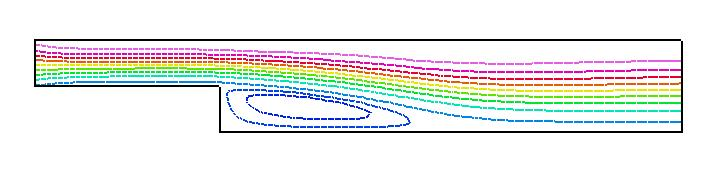
\includegraphics[width=1.0\textwidth]{lines}
\end{center}
\caption{The streamlines of the flow.}
\label{f:streamlines}
\end{figure}









\graphicspath{{./}{TimoshenkoBeamCantilever/}}
\chapter{Timoshenko beam model of a cantilever}

\modinfo{Directory}{TimoshenkoBeamCantilever}
\modinfo{Solvers}{\Idx{BeamSolver3D}}
\modinfo{Tools}{\Idx{ElmerGrid}, \Idx{Python}, \Idx{Gmsh}}
\modinfo{Dimensions}{3D, Steady-state}

\subsection*{Case definition}

In this tutorial, the geometry of a basic cantilever beam is created with Gmsh via its Python interface and simulated with Timoshenko beam elements when the applied force is a constant pressure load. Different numbers of elements for the cantilever are used to demonstrate divergence from the analytical solution for low number of elements. The workflow will be implemented in python and it demonstrates shortly how multiple simulations with different parameters can be created from a pre-existing sif-file.

\subsection*{Requirements}

Before you do this tutorial, you have to do the following things:
\begin{itemize}
   \item install the required python packages (e.g.\ via pip install) found in requirements.txt. If you do not get the exact versions, that should not matter. 
   \item replace in the file create\_geometry.py the variable of the ElmerGrid path
   \item replace in the file total\_workflow.py the variable of the ElmerSolver path
\end{itemize}
We expect the reader to have basic Python skills, but no advanced knowledge except knowing how to run a script and the ability to read the code/syntax.

\subsection*{Workflow}

If you want to see the entire workflow, simply run python total\_workflow.py.  For running its individual parts, run the single subroutines:
\begin{itemize}
    \item \textbf{create\_geometry.py:} Create the geometry via Gmsh and convert it to an Elmer usable format via ElmerGrid. Optional: you can view the geometry via the Gmsh graphical user interface.
    \item \textbf{create\_sif.py:} Take the existing constant\_pressure\_load.sif and modify it for different mesh resolutions for postprocessing files not to overwrite each other.
    \item \textbf{plot\_results.py:} Collect simulations and display them.
\end{itemize}

\subsection*{Geometry Creation}
We import the packages and functions that we need for the task. We need gmsh to create and mesh the geometry, numpy for some basic array functionality (although it could be done without it) and from the subprocess package of the basic libraries of Python the function run to use Elmergrid:
\ttbegin
from subprocess import run

import numpy as np

import gmsh 
\ttend
Enter the path to Elmergrid. If it was added to the system path already, it looks like this
\ttbegin 
elmergrid = r"ElmerGrid"
\ttend
We want to do the geometry creation repeatedly, so we define it as a function of the characteristic mesh length which determines the number of elements in the model and optionally allow the Gmsh graphical user interface (GUI) to be opened to have a final look at the geometry. 
\ttbegin 
def create_geo(lc=1e-2, gui=False):
\ttend
When starting to work on a Gmsh model, you first have to start Gmsh
\ttbegin
gmsh.initialize()
\ttend
and create the empty object 
\ttbegin
gmsh.model()
\ttend
that you will later fill with nodes, lines, surfaces etc.\ that are then meshed. We now create the start and endpoint of our beam at the positions (0,0) and (1,0). 
\ttbegin
i = 0
for x,y in zip([0.,1.],[0.,0.]):
    i = i + 1    
    gmsh.model.geo.addPoint(x, y, 0., lc, i) 
\ttend
Notice that every entity in Gmsh has a tag or index (here i). Indices start always from 1. Next we create a line to connect our nodes. This will later form our physical beam.
\ttbegin
gmsh.model.geo.addLine(1, 2, 1)
\ttend
Before geometric entities can be meshed or manipulated outside the standard Gmsh kernel, they must be synchronized with the Gmsh model creating/updating relevant internal data structures. Synchronizations can be called at any time but they are expensive, so minimize the number of synchronization points for large complicated geometries. 
\ttbegin
gmsh.model.geo.synchronize()
\ttend
In Gmsh, entities are grouped together into Physical Groups to later assign material properties, boundary conditions etc.\ to these. Usually also only the physical groups are explicitly meshed. For each group the dimension of the objects which are to be grouped is first mentioned (0 points, 1 lines, 2 surfaces, 3 bodies), then a list of the tags/ids of the objects and finally a name. Here we define our beam and the point where we apply the boundary condition:
\ttbegin
gmsh.model.addPhysicalGroup(1, [1],name = "beam")
\ttend  
\ttbegin  
gmsh.model.addPhysicalGroup(0, [1], name = "anchor")
\ttend
We then generate a mesh where the dimensionality of the intended mesh must given. As we intend to create line/beam elements, it is 1.
\ttbegin
gmsh.model.mesh.generate(1)
\ttend
As we want to study mesh convergence, we need to know the number of elements. We iterate over all existing Physical Groups, find the ones that are lines by checking the group dimension to be one and count the number of elements tags.
\ttbegin
for phys in gmsh.model.getEntities():
   if phys[0] == 1:
      eltyps, eltags, ndtags = gmsh.model.mesh.getElements(phys[0], 
                                                           phys[1]) 
      nelements = eltags[0].shape[0]
\ttend
We save the number of elements to disk in a simple csv file
\ttbegin
np.savetxt("cantilever-{0}_nelem.csv".format(str(lc)), np.array([nelements]))
\ttend
and save the mesh to the disk as well: 
\ttbegin
filename = "cantilever-{0}.msh".format(str(lc))
gmsh.write(filename)
\ttend
Gmsh automatically infers the format of the file by its ending. Optionally one can start the graphical user interface of Gmsh to inspect the geometry before finishing:
\ttbegin
if gui:
   gmsh.fltk.run()
\ttend 
We clear out the geometry
\ttbegin
gmsh.clear()
\ttend 
and close Gmsh
\ttbegin
gmsh.finalize()
\ttend 
The latter two steps must always be taken as otherwise the geometry is considered open and will linger in the background and may cause strange errors as tags of entities are still assigned and must not be reassigned as it will cause an error. We now need to convert the mesh in Gmsh format to an Elmer friendly one. We do this with ElmerGrid by calling the shell from python
\ttbegin
run([elmergrid, "14", "2", filename], shell=True, check=True)
\ttend
The check flag causes an error if the statement returns an error in the shell. If not present, this program would fail without raising an error. If you encounter problems with the latter statement, you have probably not entered the ElmerGrid path correctly. If for some reason this line does not work despite your best efforts, just comment it out
\ttbegin
#run([elmergrid, "14", "2", filename], shell=True, check=True)
\ttend
and run ElmerGrid by yourself 
\ttbegin
ElmerGrid 14 2 cantilever.msh
\ttend
by adapting the file name accordingly. We now want to see whether this program works, so we enter at the bottom of the program this standard expression
\ttbegin
if __name__ == '__main__':
\ttend 
that ensures, that this routine is only executed when you explicitly call this program file via
\ttbegin
python create_geometry.py
\ttend
and not if you call the function create\_geo from another program. We now perform a simple visual check that everything runs fine
\ttbegin
   lc = 1e0
   create_geo(lc, True)
\ttend
which should result in a geometry with one beam element. Do not get confused as Gmsh also counts the nodes as elements, so its report will mention three. The GUI output should look like Fig. \ref{fig:timoshenko-gmsh-GUI}. 

\begin{figure}[hbt]
  \centerline{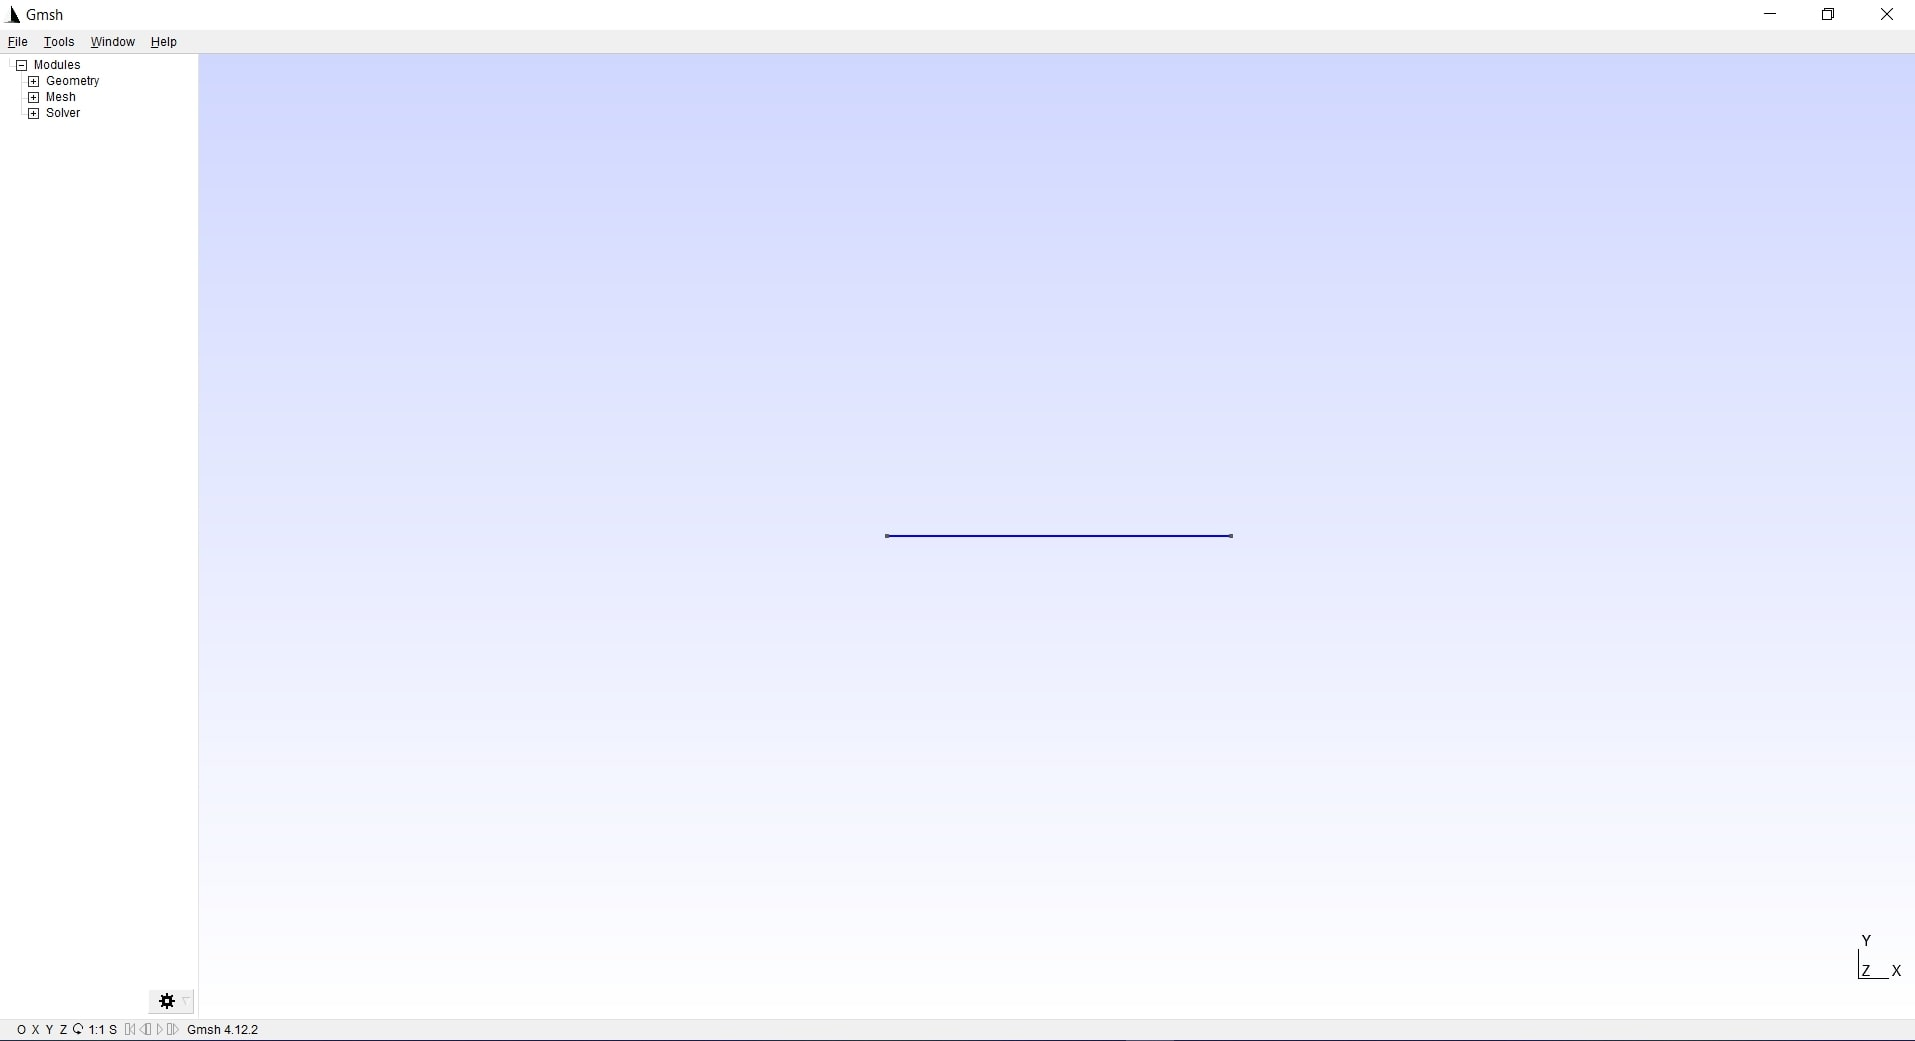
\includegraphics[width=1.0\textwidth]{gmsh-GUI}}
  \caption{Output of the Gmsh GUI.} 
  \label{fig:timoshenko-gmsh-GUI}
\end{figure}

\subsection*{Solution Procedure}
We tell Elmer to find the geometric information in the directory cantilever  
\ttbegin
Header
  Mesh DB "." "cantilever"
End
\ttend
and specify the coordinate system, some general output options and the output file in which displacements will be stored:
\ttbegin
Simulation
  Max Output Level = 5
  Coordinate System = Cartesian 3D
  Simulation Type = Steady
  Output Intervals = 1
  Steady State Max Iterations = 1
  Post File = "cantilever.vtu"
End
\ttend 
We will have later to change this automatically. Now we mention which equations, materials and body forces act on body 1
\ttbegin
Body 1
  Equation = 1
  Material = 1
  Body Force = 1
End
\ttend 
which is our only geometric object here. The material data and the geometric data of the beam have to be entered. We make a simplification here, by assuming that we have a beam shape that does not depend on the orientation of the beam with regards to loading, in other words a cylindrical beam:
\ttbegin
Material 1
 Youngs Modulus = Real 2.0e-1
 Shear Modulus = Real 1.0
 Second Moment of Area 2 = Real 1.0
 Second Moment of Area 3 = Real 1.0
 Cross Section Area = Real 1.0
 Torsional Constant = Real 1.0
 Density = 2700.0
End
\ttend 
The density is not needed here.
We specify the constant pressure load as body force acting in y-direction
\ttbegin
Body Force 1
  Body Force 1 = 0.0
  Body Force 2 = 1.0e-2
  Body Force 3 = 0.0
End
\ttend 
and set up the beam solver.
\ttbegin
Equation 1 :: Active Solvers(1) = 1

Solver 1
  Equation = "Timoshenko Beam Equations"
  Procedure = "BeamSolver3D" "TimoshenkoSolver"

  Linear System Solver = "Direct"
End
\ttend 
We can choose the most simple direct solver here as our system is quite small. Solver 2 is just a way to save some scalar data in the file cantilever.dat of the free end to later compare it with the analytic solution. We will have to change the name of the file later as well.
\ttbegin
Solver 2
  Equation = "Save Scalars"
  Exec Solver = After Timestep
  Procedure = "SaveData" "SaveScalars"
  Filename = cantilever.dat
  Variable 1 = U 1
  Variable 2 = U 2
  Variable 3 = U 3
  Variable 4 = Theta 1
  Variable 5 = Theta 2
  Variable 6 = Theta 3
  Save Points(1) = 2
End
\ttend 
We fix the first node in place
\ttbegin
Boundary Condition 1
  Target Nodes(1) = 1
  U 1 = Real 0.0
  U 2 = Real 0.0
  U 3 = Real 0.0
  Theta 1 = Real 0.0
  Theta 2 = Real 0.0
  Theta 3 = Real 0.0
End
\ttend
and are done with the simulation. No other boundary conditions need to be mentioned as everything else is free. Run the simulation by entering 
\ttbegin
ElmerSolver constant_pressure_load.sif
\ttend 
in the command line, and you should find in the directory cantilever a file called cantilever\_t0001.vtu which you can display with ParaView (Fig. \ref{fig:timoshenko-paraview}). 
\begin{figure}[hbt]
  \centerline{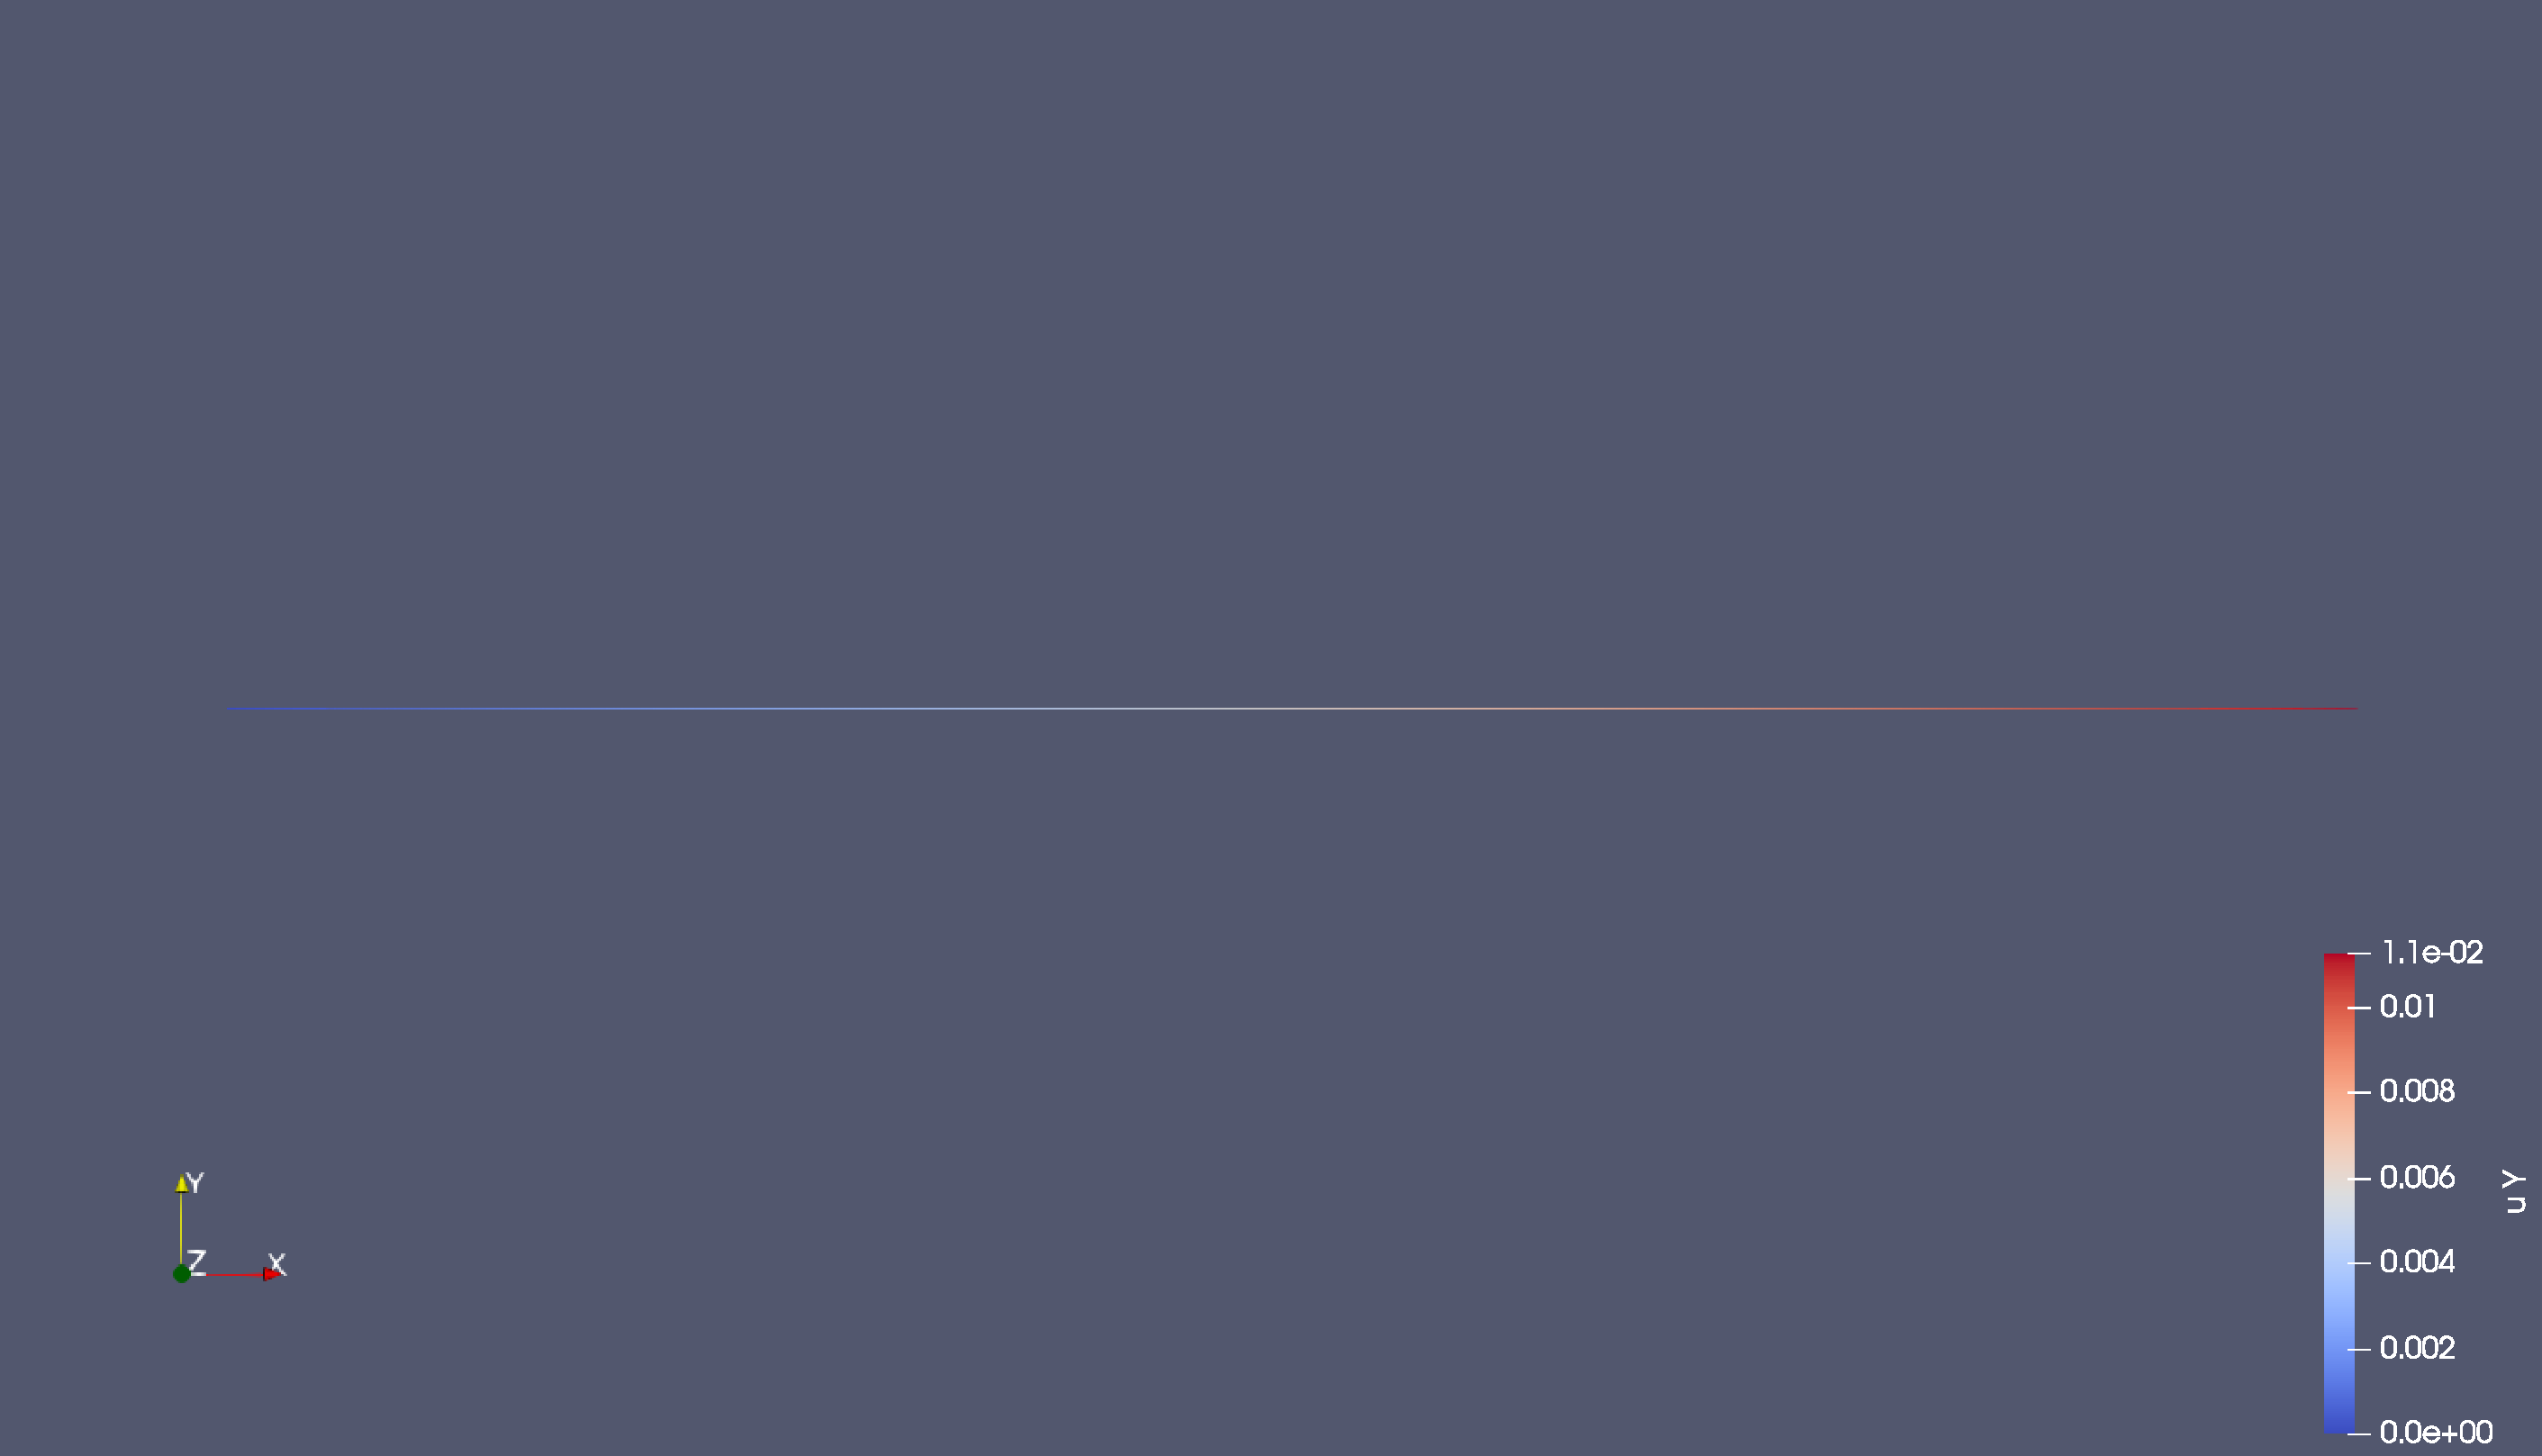
\includegraphics[width=1.0\textwidth]{displacements-paraview.pdf}}
  \caption{Output of ParaView.} 
  \label{fig:timoshenko-paraview}
\end{figure}
\subsection*{Creating New sif-Files}
We do not need to import any packages here, as everything can be done with basic Python functions. We want to update a specific sif file ad replicate it with by changing a few lines and leave 99 \% of the file untouched. Therefore as input for our function we have that file's name, a list of lines that we want to exchange and the replacements of these specific lines. The characteristic mesh length scale is there to change the name of the file. 
\ttbegin
def write_new_sif(file, 
                  search_strings, 
                  replacements,
                  lc):
\ttend 
We read the already existing sif file and all its lines. 
\ttbegin
    with open(file, 'r') as f:
        lines = f.readlines()
\ttend 
We open a new file whose name is a modified version of the already existing sif file.
\ttbegin
   with open(file.split(".")[0]+"-"+str(lc)+".sif", "w") as f:
\ttend
and iterate over all its lines.
\ttbegin
      for line in lines:
\ttend
We check each line whether a string expression is contained in that line. If not, we copy the line. Otherwise we replace it by the corresponding entry in the replacement list
\ttbegin
          flags = [string in line for string in search_strings]
          if any(flags):
             ind = [i for i,flag in enumerate(flags) if flag][0]
             f.write(replacements[ind].format(str(lc)))
          else:
             f.write(line)
    return
\ttend
We quickly test our function with the sif file for the previously generate geometry. 
\ttbegin
if __name__ == '__main__':
    lc = 1e0
\ttend
We exchange the lines that load the geometry, the output file for ParaView and the file containing the displacements of the free end with names changed appropriately for different characteristic mesh length scales.
\ttbegin 
    write_new_sif(file = "constant_pressure_load.sif", 
                  search_strings = ['  Mesh DB "." "cantilever"',
                                    '  Post File = "cantilever.vtu"',
                                    '  Filename = cantilever.dat'], 
                  replacements = ['  Mesh DB "." "cantilever-{0}"\textbackslash n',
                             '  Post File = "cantilever-{0}.vtu"\textbackslash n',
                             '  Filename = cantilever-{0}.dat\textbackslash n'],
                  lc = lc)
\ttend
Check whether the lines have been changed accordingly and move on.
\subsection*{Plotting Results}
We import numpy for some basic array functionality and matplotlib as our standard tool for creating plots in python. 
\ttbegin 
import numpy as np
import matplotlib.pyplot as plt
\ttend 
We define our function for a collection of characteristic length scales and enable optional figure saving as we do not want to dump every figure on our disc.
\ttbegin
def plot\_displacements(lcs,
                       save_fig=False):
\ttend 
For convenience we select a single font size for things like axis labels, etc.
\ttbegin
    font = 14
\ttend 
Set up two lists as collection bags for the number of elements and the displacements and start looping over the characteristic length scales 
\ttbegin
    nelems = []
    displ = []
    for lc in lcs:
\ttend 
We read the number of elements from our previously created csv file when making the geometry, directly put them into the list and do the same for the displacements created by Elmer during the solution process.
\ttbegin
        nelems.append(np.loadtxt("cantilever-{0}_nelem.csv".format(str(lc))))
        displ.append(np.loadtxt("cantilever-{0}.dat".format(str(lc)))[[4,-1]])
\ttend 
After looping we merge the displacements into one array by stacking the list entries on top of each other to receive an array with a variable number of rows and two columns (as we only read two types of displacement). We then split the displacements in two arrays for readability reasons, namely the deflection \(w\) and the rotation \(\Theta\):
\ttbegin
    displ = np.vstack(displ)
    w = displ[:,0]
    theta = displ[:,1]
\ttend 
We create a figure with one row and two columns
\ttbegin 
    fig, axs = plt.subplots(1,2,figsize=(12,8))
\ttend 
and fill each plot with the corresponding element vs.\ displacement data plotted as lines (as an alternative one could use "scatter" instead of plot to have data points instead of lines). 
\ttbegin
    axs[0].plot(nelems,w)
    axs[1].plot(nelems,theta)
\ttend 
We now calculate the analytical solutions and plot them as horizontal red lines to which our simulations should converge with increasing number of elements
\ttbegin
    A,I,G,L,E,f = 1,1,1,1,0.2,1e-2
    axs[0].axhline(y=L**4 * f * ( 1 + 4*E*I / (G*A*L**2) ) / (8*E*I), 
                   color = "r", linestyle="--")
    axs[1].axhline(y=L**3 * f / (6*E*I),
                   color = "r", linestyle="--")
\ttend 
We transform the x-axis to a logarithmic scale as the number of elements may give a large interval and is nonzero
\ttbegin
    axs[0].set_xscale("log")
    axs[1].set_xscale("log")
\ttend 
and adapt the limits of the y scale,
\ttbegin
    axs[0].set_ylim(8e-3,1.2e-2)
    axs[1].set_ylim(8e-3,8.5e-3)
\ttend 
create axis labels
\ttbegin
    axs[0].set_xlabel(r"elements",fontsize=font)
    axs[1].set_xlabel(r"elements",fontsize=font)
    axs[0].set_ylabel(r"deflection \$w\$",fontsize=font)
    axs[1].set_ylabel(r"rotation \$\textbackslash theta\$",fontsize=font)
\ttend 
and allow for the option to save our figure to the disk.
\ttbegin
    if save\_fig:
        plt.savefig("nr-elements-displacements.pdf", format="pdf",
                    bbox_inches="tight")
\ttend 
We now cause our figure to be shown on the screen as so far you should not have seen anything
\ttbegin
    # show the plot as pop up window
    plt.show()
\ttend 
and mark the end of the function by return
\ttbegin
    return 
\ttend 
Strictly speaking the latter is unnecessary as nothing is returned, but helps with readability of the code. As our usual exercise we test our program and you should end up with a single plotted data point.
\ttbegin
if __name__ == '__main__':
    plot_displacements(lcs = np.array([1e0]))
\ttend
\subsection*{Total Workflow for Mesh Convergence Study}
In this section we piece together all our previous programs. We need subprocess.run again for calling Elmersolver and numpy for basic array routines.
\ttbegin
from subprocess import run

from numpy import array
\ttend 
We import all our previously created functions
\ttbegin
from create_geometry import create_geo
from create_sif import write_new_sif
from plot_results import plot_displacements
\ttend 
and add our path to ElmerSolver.
\ttbegin
elmersolver = "ElmerSolver"
\ttend 
We now write the main routine of our solver, create some array with a collection of characteristic length scales that we would like to use and start iteration. (If lc is larger than 1, you will end up with just 1 element, so lc = 1 is the sensible upper bound here)
\ttbegin
if __name__ == '__main__':
    lcs = array([1e0,1e-1,1e-2,1e-3])
    for lc in lcs:
\ttend 
We create the geometry and mesh it with Gmsh to convert it to an Elmer compatible file format
\ttbegin
        create_geo(lc)
\ttend 
and create the corresponding sif file whose geometry input location and its result output files are changed to avoid overwriting previous results.
\ttbegin
        write_new_sif(file = "constant_pressure_load.sif", 
                      search_strings = ['  Mesh DB "." "cantilever"',
                                 '  Post File = "cantilever.vtu"',
                                 '  Filename = cantilever.dat'], 
                      replacements = ['  Mesh DB "." "cantilever-{0}"\textbackslash n',
                                 '  Post File = "cantilever-{0}.vtu"\textbackslash n',
                                 '  Filename = cantilever-{0}.dat\textbackslash n'],
                      lc = lc)
\ttend 
We call Elmer solver to solve the system of equations
\ttbegin
        run([elmersolver,
             "constant_pressure_load-{0}.sif".format(str(lc))],
            shell=True, 
            check=True)
\ttend 
and continue to the next iteration or stop the iteration process. In the end we plot our accumulated results
\ttbegin
    plot_displacements(lcs, True) 
\ttend
which should show a plot similar to Fig.\ \ref{fig:timoshenko-results}. 

\begin{figure}[hbt]
  \centerline{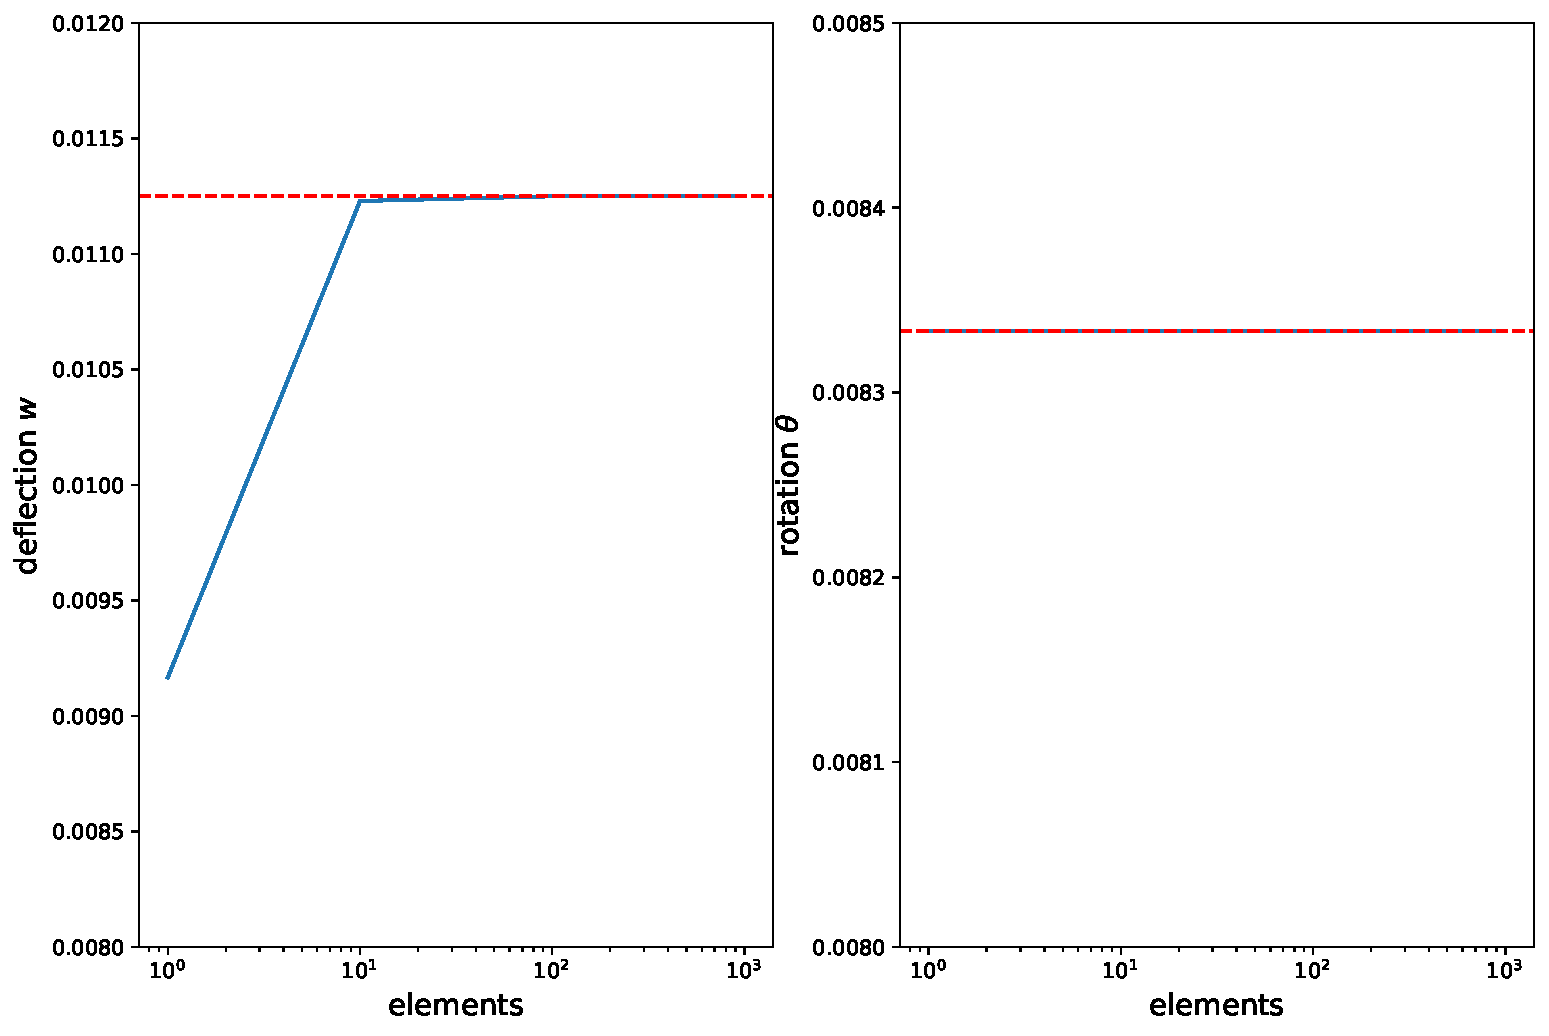
\includegraphics[width=1.0\textwidth]{nr-elements-displacements.pdf}}
  \caption{Collected results.} 
  \label{fig:timoshenko-results}
\end{figure}

\subsection*{Concluding Remarks}

So far this tutorial has presented a minor introduction to the use of the Timoshenko beam solver and applying Elmer in conjunction with Gmsh and also exemplified the usefulness of Python for the construction of workflows to study mesh convergence. For the inexperienced use, we would like to mention that mesh convergence is not usually done with the help of analytical solutions as they are only available in a few cases. Instead one typically analyses the development of the residuals and target outcomes of interest. It goes without saying that if the residuals do not decrease with increasing mesh refinement, you are not converging and you should check the physics and numerics of your problem. 

\vfill
\mbox{}



% Under construction
%\graphicspath{{./}{elast_elstat_beam3d/}}
%\chapter{Electrostatically loaded 3D elastic beam}

\modinfo{Solvers}{\Idx{StressSolve}, Idx{StatElecSolve}}
\modinfo{Tools}{\Idx{ElmerGrid}, editor}
\modinfo{Dimensions}{3D, Steady-state}

\section{Case definition}


\section{Results}

\begin{figure}[h]
  \centerline{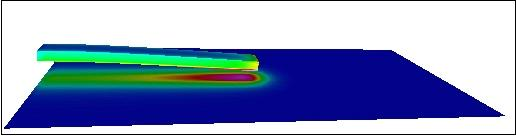
\includegraphics[width=0.8\textwidth]{electric_force}}
  \caption{An elastic beam bended by the electrostatic force due to a
          potential difference between the beam and the bottom
          plate. The electric potential is calculated in the volume
          surrounding the beam although the solution or the mesh are
          not shown.}
\end{figure}



% Now these are truly obsolete so let's not include them any more
%\part{Obsolete Problems}

%These tutorials have become obsolete due to the transition from 
%ElmerFront to ElmerGUI. If you still want to continue using ElmerFront these
%tutorials may be perfectly valid.

%\graphicspath{{./}{TemperatureAngle/}}
%\chapter{Temperature distribution of a toy glacier}

\modinfo{Directory}{ToyGlacierTemperature}
\modinfo{Solvers}{\Idx{HeatSolver}} 
\modinfo{Tools}{\Idx{ElmerGUI},\Idx{nglib}} 
\modinfo{Dimensions}{2D, Steady-state}
\modinfo{Author}{Peter R{\aa}back, Thomas Zwinger}


\subsection*{Introduction}

The purpose of this simple tutorial is to be an introduction into Elmer for people dealing with computational glaceology.
This tutorial shows how to apply one equation and related boundary conditions to just one domain.


\subsection*{Problem description}

Consider a 2D toy model of a glacier with length of 7000~m and thickness of about 1000~m. 
There is a slight declination in the geometry which will make the glacier flow to the left. 
The left-hand-side is rounded to imitate a true glacier while the right-hand-side is 
cut off. 

\begin{figure}
\begin{center}
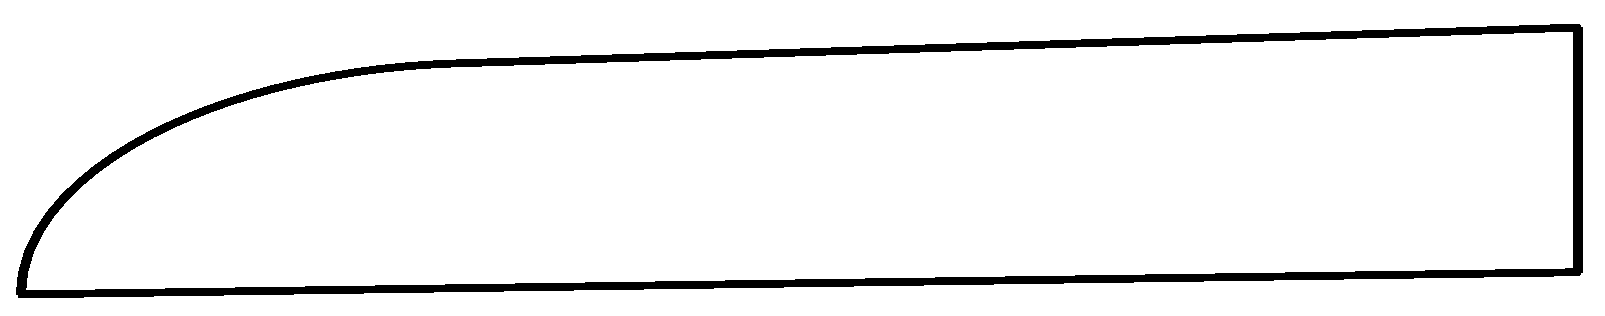
\includegraphics[width=120mm]{glacier_toy_shape}
\caption{The shape of the toy glacier to be studied}\label{glac:shape}
\end{center}
\end{figure}

We solve for the temperature distribution $T$ of the glacier. 
A heat flux of $q=0.02$~W/m$^2$ is applied at the bottom of the glacier while the surface stays at a
fixed temperature of $T_0=-10$~C. The material properties of ice are used for the 
heat conductivity $\kappa(T)$. 
The temperature distribution in the glacier 
may be solved from
\begin{equation}
\left \{
\begin{array}{cccc}
- \kappa \Delta T &= & 0 & \mathrm{ in } \, \, \Omega \\
T&=&T_0 & \mathrm{ on } \, \, \Gamma_D \\
\kappa \frac{\partial T}{\partial n} &=& q & \mathrm{ on } \,\, \Gamma_N \\
\end{array}
\right .
\end{equation}

\subsection*{Starting and meshing}

Start \texttt{ElmerGUI} from command line or by clicking the icon in your desktop (or in the /bin directory of you installation). 
Here we describe the essential steps in the ElmerGUI by writing out the clicking procedure. Tabulation generally means that the 
selections are done within the window chosen at the higher level. 

The mesh is given in ElmerGrid format in file \texttt{glacier\_toy.in2d} in the samples directory of ElmerGUI, 
load this file.
\ttbegin
File 
  Open -> glacier\_toy.in2d
\ttend
You should obtain a mesh consisting of just two triangular elements. The mesh is created by the \texttt{netgen} plugin 
and in order to increase the mesh density the in-line parameters of netgen must be defined in ElmerGUI.
Here we set the maximum element size to 50. 
\ttbegin
Mesh
  Configure... 
    nglib -> Max H: 50
\ttend
The resulting mesh should consist of 3335 nodes and 6355 triangles as may be checked in the 
\texttt{Model summary} window.
%If the mesh was successfully imported your window should look something in figure~\ref{glac:mesh}.

%\begin{figure}
%\begin{center}
%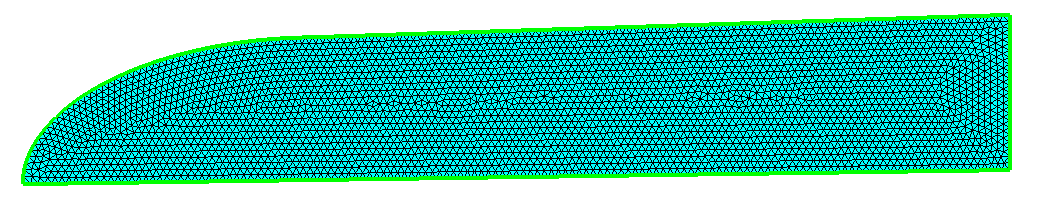
\includegraphics[width=120mm]{glacier_toy_mesh}
%\caption{The finite element mesh in ElmerGUI}\label{glac:mesh}
%\end{center}
%\end{figure}

\subsection*{Command file definition}

After we have the mesh we start to go through the Model menu from the top to bottom. 
In the \texttt{Setup} we choose things related to the whole simulation such as file names, 
time stepping, constants etc.
The simulation is carried out in 2-dimensional cartesian
coordinates and in steady-state. 
Only one steady-state iteration is needed as the case is linear. 
\ttbegin
Model
  Setup 
    Simulation Type = Steady state
    Steady state max. iter = 1
\ttend
Choose \texttt{Accept} to close the window.

In the equation section we choose the relevant equations and parameters related to their solution. 
In this case we'll have one set only one equation -- the heat equation.


When defining Equations and Materials it is possible to assign the to bodies immediately, or to use mouse
selection to assign them later. In this case we have just one body and one boundary and therefore its easier to assign 
the Equation and Material to it directly.

For the linear system solvers we are happy to use the defaults. One may however, try out different
preconditioners (ILU1,\ldots) or direct Umfpack solver, for example.
\ttbegin
Model
  Equation
    Add 
      Name = Heat Equation
      Apply to bodies = 1
      Heat Equation
        Active = on
  Apply   
  OK
\ttend        

The Material section includes all the material parameters.
They are divided to generic parameters which are direct properties of the material
without making any assumptions on the physical model, such as the mass. Other properties assume
a physical law, such heat conductivity.
We choose ice from the Material library which automatically sets for the needed material properties. 
\ttbegin
Model
  Material
    Add 
      Material library
        Water (frozen)
      Apply to bodies = Body 1 
      Add 
      OK
\ttend
This includes, for example, temperature dependent heat conductivity as may be seen under the HeatEquation page of
the material properties. MATC language is used here to define the functional form.


A Body Force represents the right-hand-side of a equation that in this case represents
the heat source. In this case there are no internal heat sources so we do not need one.
Also no Initial Condition is required in steady state case.

\begin{figure}
\begin{center}
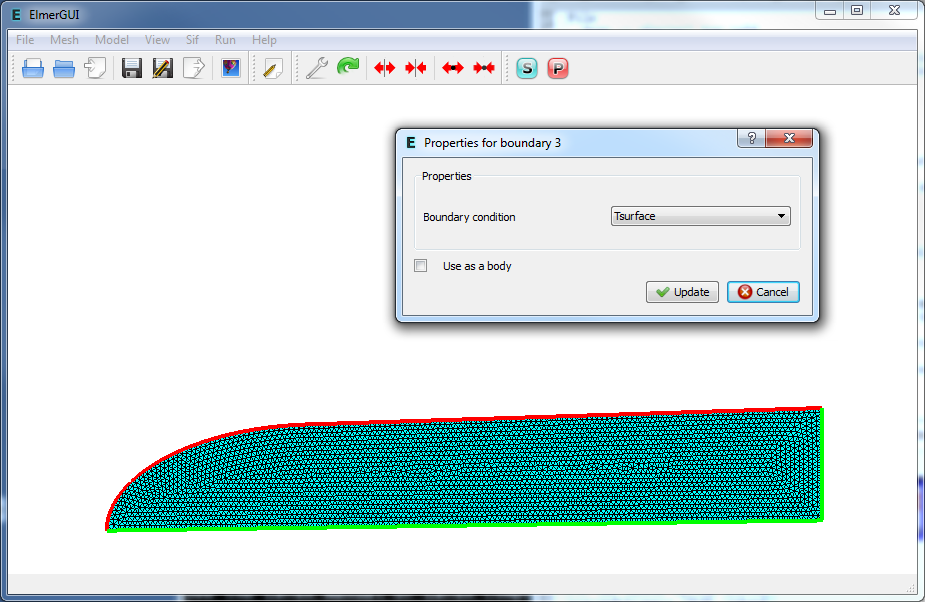
\includegraphics[width=120mm]{glacier_toy_gui}
\caption{Defining boundary conditions in ElmerGUI session}\label{glac:bc}
\end{center}
\end{figure}

We set three different kinds of boundary conditions. A fixed temperature, a fixed 
flux and natural boundary condition (zero flux). As there are several boundaries
we first define the different boundary types, and thereafter assign them using the mouse.
A screenshot of the case when setting the BCs is shown in figure~\ref{glac:bc}.

\ttbegin
Model
  BoundaryCondition
    Add 
      Heat Equation
        Temperature = -10.0
      Name = Tsurface
      OK
    Add 
      Heat Equation
        Heat Flux = 0.02
      Name = Tflux
      OK
    Add 
      Name = Tnatural
      OK
\ttend   
Then we set the boundary properties 
\ttbegin
Model 
  Set boundary properties  
\ttend
Choose the correct boundary by clicking with the mouse
and apply the condition for this boundary.
\ttbegin
Boundary condition
  Click top boundary -> choose Tsurface
  Click bottom boundary -> choose Tflux
  Click r.h.s. boundary -> choose Tnatural
\ttend

\subsection*{Saving and solution}

For the execution 
ElmerSolver needs the mesh files and the command file. We have know basically defined
all the information for ElmerGUI to write the command file. After writing it we may also visually 
inspect the command file.
\ttbegin
Sif 
  Generate
  Edit -> look how your command file came out  
\ttend

Before we can execute the solver we should save the files in a directory. In saving the project all the
necessary files for restarting the case will be saved to the 
destination directory.
\ttbegin
File 
  Save Project
\ttend

After we have successfully saved the files we may start the solver
\ttbegin
Run
  Start solver
\ttend
A convergence view automatically pops up showing relative changes of each iteration.
The heat conductivity of ice is set to be dependent on temperature and this results to a 
nonlinear iteration.
The resulting output is shown in figure~\ref{glac:conv}.

\begin{figure}
\begin{center}
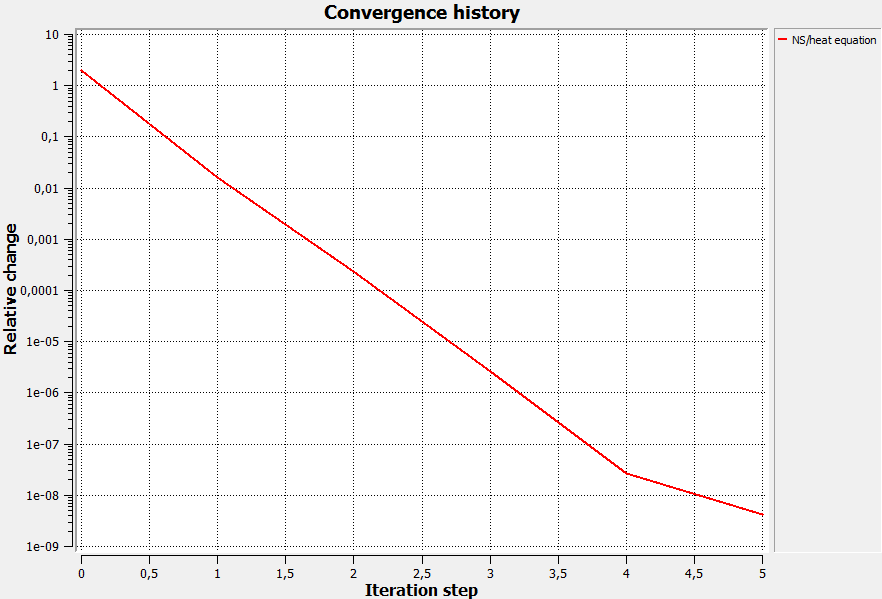
\includegraphics[width=100mm]{glacier_toy_convergence}
\caption{The convergence  ElmerGUI}\label{glac:conv}
\end{center}
\end{figure}

Note: if you face problems in the solution phase and need to edit the setting, always remember to save
the project before execution.

\subsection*{Results}

To view the results we use Paraview,
\ttbegin
Run
  Start Paraview
\ttend
Picture~\ref{glac:figtemp} shows
the surface mesh colored with temperature.
Note that these results were carried out with the obsolite
VTK based tool within ElmerGUI, and therefore look different than in Paraview.

\begin{figure}
\begin{center}
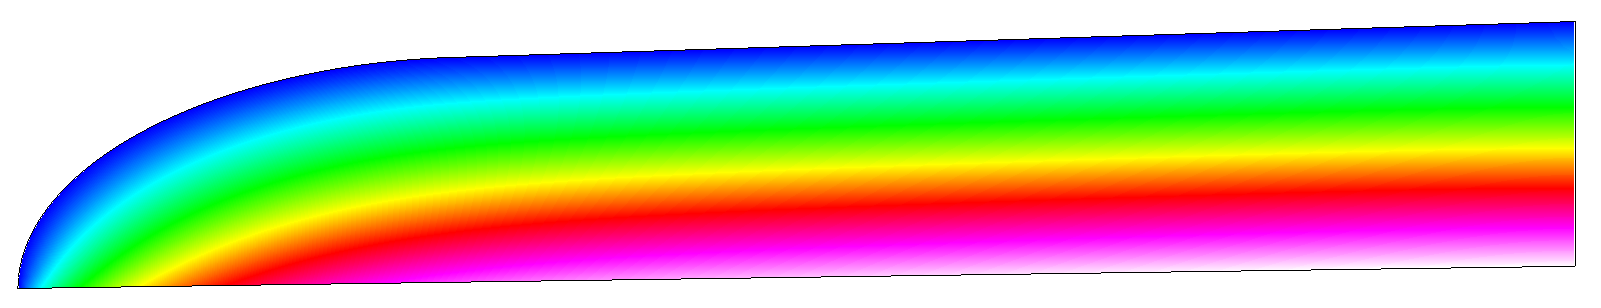
\includegraphics[width=120mm]{glacier_toy_temp}
\caption{The temperature distribution of the toy glacier.}\label{glac:figtemp}
\end{center}
\end{figure}


The maximum temperature obtained with the above choices is 0.11166~C. 
With a denser mesh the result is
naturally more accurate, but solving the problem takes more calculation time.

You may study the effect of mesh refinement by choosing 
a different value for the \texttt{Max H} parameter.
under \texttt{Configure}. After choosing \texttt{Remesh} and saving the mesh 
the solver may be recalled with the modified mesh.


\section*{Transient simulation}

We use the steady-state simulation presented above as our starting point and 
solve a transient version of it. Initially the glacier is assumed to be at -10~C 
and it is gradually heated from below. 


We use 2nd order bdf time-stepping method is selected with 100 steps
and with step size of 100 years - melting the ice from below with such a small flux 
would take quite a few years. 
The mathematical expression followed 
by ``\$'' is evaluated when the command file is read.
Here it is used to transform the time in years to those in one second. 
\ttbegin
Model
  Setup 
    Simulation Type = Transient
    Time Stepping Method = bdf
    BDF Order = 2
    Time Step Intervals = 100
    Time Step Sizes = \$ 3600 * 24 * 365.25 * 100
    Gravity = ...
\ttend

Initial conditions should be given to transient cases. In this case we choose a constant Temperature 
of -10~C. This is consistant with the boundary condition at the top wall.
\ttbegin
Model
  Initial Condition 
    Name = Initial Guess
    Heat Equation
      Temperature = -10.0
\ttend

\begin{figure}
\begin{center}
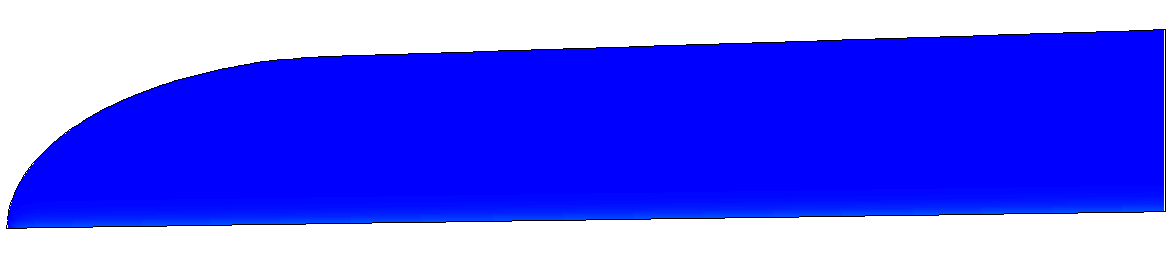
\includegraphics[width=120mm]{glacier_t1}
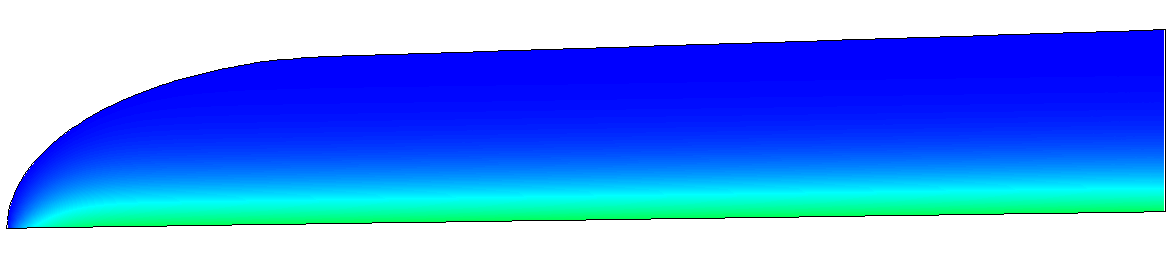
\includegraphics[width=120mm]{glacier_t20}
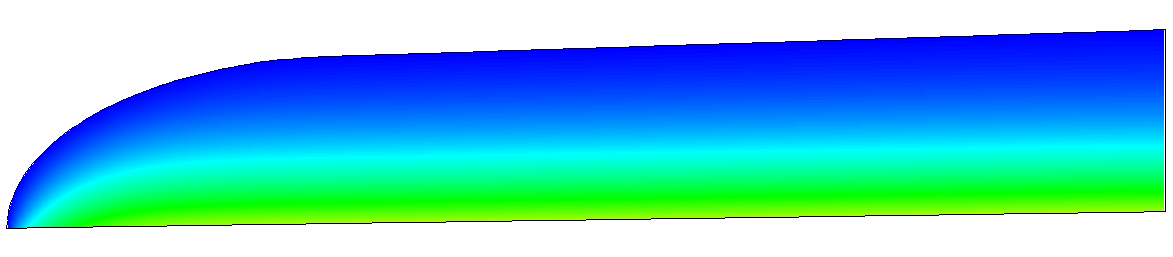
\includegraphics[width=120mm]{glacier_t50}
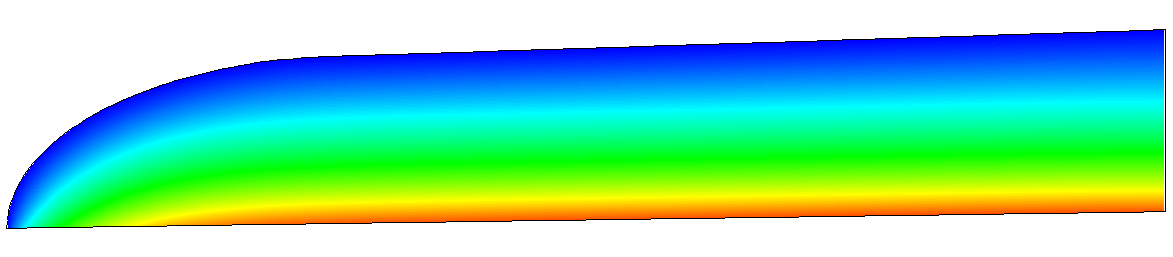
\includegraphics[width=120mm]{glacier_t100}
\caption{Temperature distribution after 1, 20, 50 and 100 timesteps. The temperature scale is the 
same that is used in the steady-state case. The maximum temperature at end should be about -3.7611~C.}
\end{center}
\end{figure}

\hfill
\mbox{}








%\graphicspath{{./}{ElasticBeam/}}
%\chapter{Loaded elastic beam}

\modinfo{Directory}{ElasticBeam}

\section{Solution with linear model} 


\modinfo{Solvers}{\Idx{StressSolve}}
\modinfo{Tools}{\Idx{ElmerFront}}
\modinfo{Dimensions}{2D, Steady-state}

\subsection*{Case definition}

A homogenous, elastic beam ($\Omega$) is rigidly supported on one 
end (boundary $\Gamma_4$). On boundary $\Gamma_3$ the beam is subjected 
to a load $q(x)$, which grows linearly from zero to $q_0$ 
(see figure~\ref{fg:beam}). Material properties of the beam are the Poisson 
ratio 0.3 and Young's modulus $200\cdot 10^9$N/m$^2$. Problem is to solve the 
displacement of the beam.  

\begin{figure}[h]
\centering
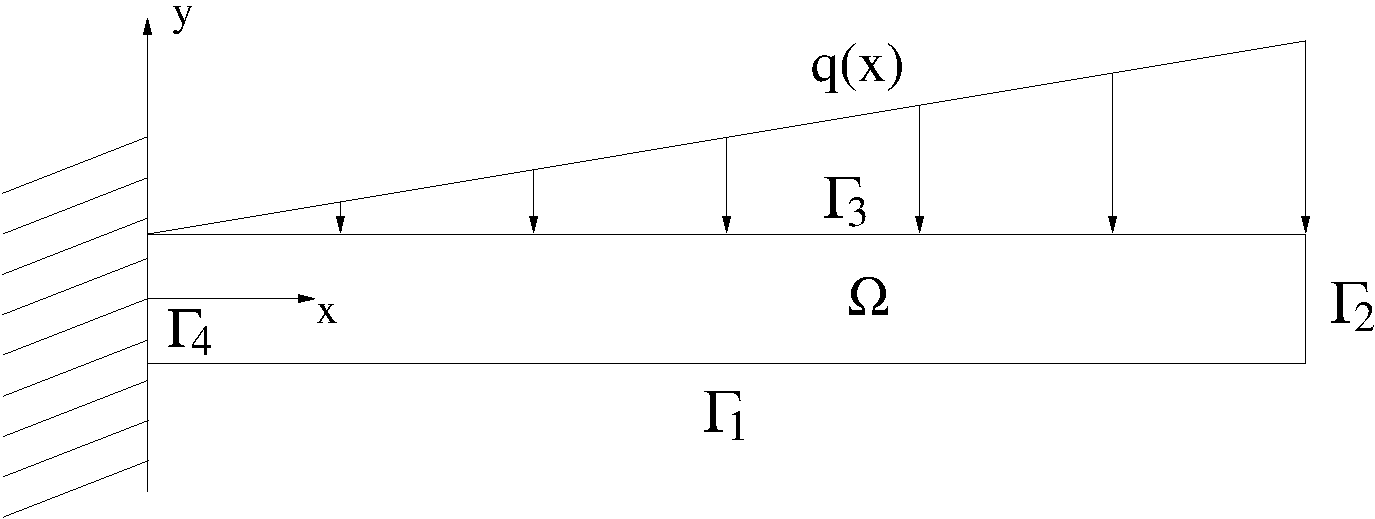
\includegraphics[width=100mm]{Beam}
\caption{Beam and loading.}\label{fg:beam}
\end{figure}

Problem is solved according to linear elasticity theory. Mathematically 
the problem to be solved is
\begin{equation}
\left \{
\begin{array}{rcll}
-div \sigma & = & 0 & \mbox{ in } \Omega \\
\sigma & = & \lambda tr [\varepsilon(u)]I + 2 \mu \varepsilon(u) &
\mbox{ in } \Omega \\
u & = & 0 & \mbox{ on } \Gamma_4 \\
\sigma n & = & 0 & \mbox{ on } \Gamma_1 \cup \Gamma_2 \\
\sigma n & = & -q & \mbox{ on } \Gamma_3 \\
\end{array}
\right .
\end{equation}
where $\lambda$ and $\mu$ are the Lam\'{e} constants (which can be expressed 
in terms of the Poisson ratio and Young's modulus), $\varepsilon$ is the 
linearized strain tensor, $u$ is the displacement vector, $q$ is the given
surface traction and $n$ is the outward unit normal to the boundary.

\subsection*{Solution procedure}

\begin{itemize}
\item Start ElmerFront.
\item Open the file that contains the geometry of the beam from 
the File menu. Select also the working directory for the model.
\ttbegin
File -> Open cad-file 
  File = Beam.egf 
  Model name = Beam 
  Model directory = beam_tutorial
\ttend
\item Select the equations to be solved from the Problem menu. In this 
case stress analysis is selected. It solves the problem according to 
linear elastic theory. 
\ttbegin
Problem -> Equations 
  Stress analysis 
\ttend
\item Define the material properties from the Model menu. Give the values for 
Young's modulus and the Poisson ratio. Add the defined material 
properties to the material property sets so they become attached 
to $\Omega$. 
\ttbegin
Model -> Materials 
  Young's modulus = 200e9 
  Poisson ratio = 0.3
\ttend

\item Define the Dirichlet boundary condition and the load from the
Model menu. Give the value zero for displacements at the boundary
$\Gamma_4$ and press Add. The linearly varying load is defined in the
same panel as follows.  Select the boundary~3, click the cursor on to
the Force-y line, check the box Table, and press finally the Edit
button. A window opens in which the tabular bc entry is
defined. Select first Coordinate 1 as the variable on which the
Force-y depends. Write on the line below entry {\tt 0 0}. Click
Add. Write {\tt 1 -1.0e7} on the line and click again Add. Now, the
space below contains two lines written in two columns. The first
colums holds the values for the Coordinate~1 and the second column for
the Force-y. The value of the force is interpolated according to these
definitions. Now click OK on the Table entry panel. In Boundary
Conditions panel, click Add and then OK.
\ttbegin
Model -> Boundary conditions
Boundary 4
Displacement-X = 0
Displacement-Y = 0
Add
Boundary 3
Force-Y
Table
Edit
Variable = Coordinate 1
0 0
Add
1 -1e7
Add
OK
Add
OK
\ttend

\item Define mesh from the Mesh menu. First give name for the
mesh. Then select ``Mesh structure'' and define element type and the
number of elements. Attach the defined mesh structure to the Body~1
and click OK. Create the mesh by pressing ``Generate mesh'' button.

\ttbegin 
Mesh -> Define mesh 
Mesh name = Mesh1 
Mesh structure 
Element type = Quad 
Nof elements (1st and 3rd edge) = 40 
Nof elements (2nd and 4th edge) = 4 
Add 
OK 
Generate mesh 
\ttend
\item Now to solve the problem defined with the constant load select from 
the Run menu item Solver. 
\ttbegin
Run -> Solver 
\ttend
\item Results may be viewed with the ElmerPost program
\ttbegin
Run -> Postprocessor
\ttend
or click the {\tt Results} button on the main window.
\end{itemize}

\subsection*{Results}

As a result the absolute value of maximum displacement is given. The 
displacements calculated with different load values $q_0$ are tabulated in 
table~\ref{tb:struct3a}. Note that the absolute value of the
displacement varies linearly with respect to the load since the model
is linear.

\begin{figure}[h!]
\begin{center}
  
\includegraphics[width=0.30\textwidth,angle=0]{respic1.png}
  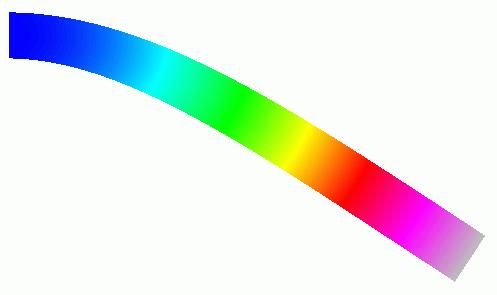
\includegraphics[width=0.28\textwidth,angle=0]{respic2.png}
  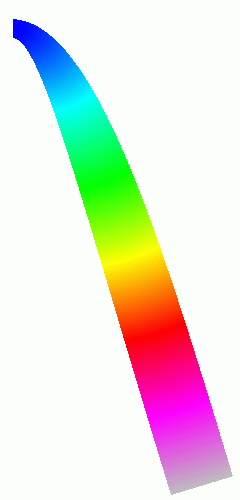
\includegraphics[width=0.25\textwidth,angle=0]{respic3.png}
  \caption{The displacement of an elastic beam with different loads
using a linear model}
  \label{fig:elast_beam1}
\end{center}
\end{figure}

\begin{table}[h]
\caption{Displacements with different load values}
\label{tb:struct3a}
\begin{center}
\begin{tabular}{ll} \hline
$q_0$ [N/m$^2$] & $\max |u|$ [m] \\ \hline
-1.0$e7$ & 0.04862 \\
-1.0$e8$ & 0.4862 \\
-1.0$e9$ & 4.862 \\ \hline
\end{tabular}
\end{center}
\end{table}

If you look at the results you can see that the displacement values
become relatively large. The linear theory is valid only to small 
displacements. From Fig~\ref{fig:elast_beam1} you can also notice that the
beam does not maintain its original form. This means that the linear 
elasticity theory can not take into consideration all the necessary 
phenomenona that are related to the problem, anymore. To be able to 
solve the problem we must use general elasticity theory. This is done 
in the following subsection.


\section{Solution with nonlinear model}

\modinfo{Solvers}{\Idx{ElasticSolve}}
\modinfo{Tools}{editor}
\modinfo{Dimensions}{2D, Steady-state}

\subsection*{Case definition}

In the following the beam problem is solved with general elasticity theory.
That is done by using the nonlinear elasticity solver of Elmer. 
In the case of homogenous 
elastic material the problem can be written into a following mathematical form

\begin{equation}
\left \{
\begin{array}{rcll}
-div [(I+ \nabla u) \Sigma] & = & 0 & \mbox{ in } \Omega \nonumber \\
\Sigma & = & \lambda (tr E)I + 2 \mu E & \mbox{ in } \Omega \nonumber \\
E & = & \frac{1}{2}(\nabla u^{T} + \nabla u + \nabla u^{T} \nabla u) & 
\mbox{ in } \Omega \nonumber \\
u & = & 0 & \mbox{ on } \Gamma_4 \\
(I+ \nabla u)\Sigma n & = & 0 & \mbox{ on } \Gamma_1 \cup \Gamma_2 \\
(I+ \nabla u)\Sigma n & = & -q & \mbox{ on } \Gamma_3 \\
\end{array}
\right .
\end{equation}
where $u$ is the displacement vector, $q$ is the given surface load, $\Sigma$ 
is the second Piola-Kirchhoff stress tensor, $\lambda$ and $\mu$ are the 
Lam\'{e} constants and $E$ is the Green-St Venant strain tensor.


\subsection*{Solution procedure}

The problem is solved here without the graphical user interface.
Open the solver input file of the linear case, Beam.sif, and edit the
following changes. Define nonlinear elasticity as the only equation
\ttbegin
Equation 1
  Name = "Equation1"
  Nonlinear Elasticity = Logical True
End
\ttend

Change the name correspondingly in the Solver block and add
information about the procedure needed. Leave all other keywords on
the solver block unchanged.
\ttbegin
Solver 1
  Equation = "Nonlinear Elasticity"
  Procedure = "ElasticSolve" "ElasticSolver"
...
End
\ttend

Finally, the force load may be changed in boundary condition 2 as
\ttbegin
  Force 2 = Variable Coordinate 1
      0 0
      1 -1.0000e+09
    End
\ttend

The problem may now be solved from the command line by typing {\tt
ElmerSolver}.

\subsection*{Results}

\begin{table}[tbhp]
\caption{Maximum displacements with different load values calculated according to 
general elasticity theory and linear theory.}
\label{tb:struct3b}
\begin{center}
\begin{tabular}{lll} \hline
$q_0$ [N/m$^2$] & 
$\max |u|$ [m] &
$\max |u|$ (linear) [m] \\ \hline
-1.0e$^7$ & 0.04890 & 0.04862 \\
-1.0e$^8$ & 0.4532 & 0.4862  \\
-1.0e$^9$ & 1.297  & 4.861 \\ \hline
\end{tabular}
\end{center}
\end{table}

From table~\ref{tb:struct3b} you can see the difference between the 
results calculated according to nonlinear and linear theory. According to 
the linear theory the displacement increases linearly as the load 
increases. This can be seen clearly from the results. The last loading
level (-1.0e9 N/m$^2$) is fairly large and the beam would probably break 
under that load. So the value of displacement might be unrealistic in that
case.   


\vfill
\mbox{}


%\graphicspath{{./}{FlowStepIncompressible/}}
%\chapter{Incompressible flow passing a step}
\label{tut:stepflow}

\section{Solution with linear triangles}

\modinfo{Directory}{FlowStepIncompressible}
\modinfo{Solvers}{\Idx{FlowSolve}}
\modinfo{Tools}{\Idx{ElmerFront}}
\modinfo{Dimensions}{2D, Steady-state}


\subsection*{Case definition}

A fluid, flowing past a step (see figure~\ref{fg:struct2}), has the density
1~kg/m$�$ and viscosity 0.01~kg/ms. The velocity of the fluid on the 
incoming boundary $\Gamma_6$ in the x-direction is 1~m/s and in 
the y-direction 0~m/s (see figure~\ref{fg:struct2}). On the outcoming boundary 
$\Gamma_4$ the velocity is 0~m/s in the y-direction and the pressure
is 0~Pa. The problem is to solve the velocity field and the pressure 
change in $\Omega$.

\begin{figure}[h]
\centering
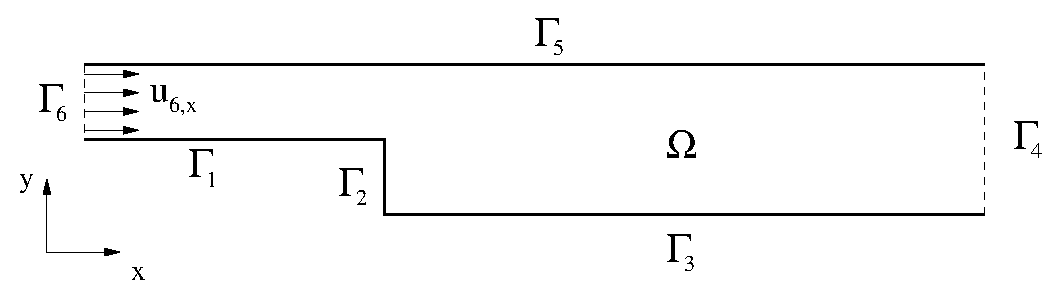
\includegraphics[width=100mm]{Body1}
\caption{Step.}\label{fg:struct2}
\end{figure}

Mathematically the problem to be solved is
\begin{equation}
\left \{
\begin{array}{rccl}
- \nabla \cdot (2 \mu \overline{\overline{\varepsilon}}) + \rho 
\vec{u} \cdot \nabla \vec{u} + \nabla p & = & 0 & \mbox{ in } \Omega \\
\nabla \cdot \vec{u} & = & 0 & \mbox{ in } \Omega \\
\end{array}
\right .
\end{equation}
with the boundary conditions
\begin{equation}
\left \{
\begin{array}{rccl}
\vec{u}_{x} & = & 1 & \mbox{ on } \Gamma_6 \\
\vec{u}_{x} & = & 0 & \mbox{ on } \Gamma_i ,\: i=1,2,3,5 \\
\vec{u}_{y} & = & 0 & \mbox{ on } \Gamma_i ,\: i=1,\ldots,6, 
\end{array}
\right .
\end{equation}
where $\mu$ is the viscosity, $\overline{\overline{\varepsilon}}$ is 
the strain tensor,  $\rho$ is the density, $\vec{u}$ is the velocity and
$p$ is the pressure. It is assumed that the density and viscosity are 
constants. 

\subsection*{Solution procedure}

\begin{itemize}
\item Start ElmerFront.
\item Open the file that contains the geometry of the step from 
the File menu. Select also the working directory for the model.
\ttbegin
File -> Open cad-file 
  File = StepFlow.egf 
  Model name = StepFlow 
  Model directory = step_tutorial
\ttend
\item Select the equations to be solved from the Problem menu. In this 
case we solve the Navier-Stokes equations.
\ttbegin
Problem -> Equations 
  Navier-Stokes 
\ttend
\item Define the material properties from the Model menu. Give the values for 
the density and the viscosity.
\ttbegin
Model -> Materials 
  Density = 1 
  Viscosity = 0.01
\ttend
\item Define boundary conditions from the Model menu. Give the values of 
the velocities at each boundary \begin{math}\Gamma_i\end{math}. Add the 
different boundary conditions to boundary condition sets and attach each 
constraint to a boundary or boundaries \begin{math}\Gamma_i\end{math} that 
the constraint concerns (see figure~\ref{fg:struct2}).
\ttbegin
Model -> Boundary conditions 
  {\it on }\begin{math}{\Gamma_6}\end{math}: Velocity-X = 1 and Velocity-Y = 0 
  {\it on }\begin{math}\Gamma_i,\: i=1,2,3,5\end{math}: Velocity-X = 0 and Velocity-Y = 0 
  {\it on }\begin{math}\Gamma_4\end{math}: Velocity-Y = 0
\ttend
\item Define mesh from the Mesh menu. First give name for 
the mesh and then define the element size. Create the mesh by pressing
``Generate mesh'' button. 
\ttbegin
Mesh -> Define mesh 
  Mesh name = Mesh1 
  Model Mesh H [m] = 0.2 
  Generate mesh
\ttend
\item Now to solve the problem select from the Run menu item Solver. This 
starts the solver. 
\ttbegin
Run -> Solver 
\ttend
\item After the solution is done, view the results by selecting from the Run
menu item Postprocessor. 
\ttbegin
Run -> Postprocessor 
\ttend
\item To save the created model, select from the File menu item Save 
model file. 
\ttbegin
File -> Save model file 
\ttend
\item To exit Elmer select from the File menu item Exit. 
\ttbegin
File -> Exit
\ttend
\end{itemize}

\subsection*{Results}

As a result the maximum pressure difference and maximum velocity is 
given (see table~\ref{tb:struct2}). One special result of interest 
is the point, on the x-axis, at which the direction of the flow changes. 
In this case its position is about 8.3 m. 
   
\begin{table}[h]
\caption{Pressure difference and velocity}
\label{tb:struct2}
\begin{center}
\begin{tabular}{lll} \hline
Elements & $\max (\Delta p)$ [Pa] & $\max |\vec{u}|$ [m/s] \\ \hline
1426  & 1.039  & 1.489 \\ \hline
\end{tabular}
\end{center}
\end{table}



\section{Solution with 2nd order rectangles}

\modinfo{Solvers}{\Idx{FlowSolve}}
\modinfo{Tools}{\Idx{ElmerGrid}, editor}
\modinfo{Dimensions}{2D, Steady-state}

\subsection*{Case definition}

In the following the flow past a step -problem is solved with
eight-noded quadrilateral elements. The mesh is done with ElmerGrid
which is a simple mesh generator that can be downloaded via the Elmer
internet pages. Here a grd file is introduced. It contains the
geometry data and parameters needed in defining the mesh of the
structure. ElmerGrid transforms this file into Elmer mesh files
(mesh.boundary, mesh.nodes, mesh.header and mesh.elements).



\subsection*{Solution procedure}

The problem might be solved using ElmerFront by reading an external
mesh into the program but here instructions for command line usage of
Elmer are given.
\begin{itemize}
\item First generate mesh with ElmerGrid with the following command.
\ttbegin 
ElmerGrid 1 2 Step.grd
\ttend

\item Make the necessary changes to the .sif file. Changes are made to
header section, boundary conditions and boundaries. The sif file is
conveniently edited using a text editor. The sections should be edited
into the following form
\ttbegin 
Header
  CHECK KEYWORDS Warn
  Mesh DB "." "Step"
End

Boundary Condition 1
  Name = "Constraint1"
  Target Boundaries(1) = 1

  Velocity 1 = 1
  Velocity 2 = 0
End

Boundary Condition 2
  Name = "Constraint2"
  Target Boundaries(1) = 3

  Velocity 1 = 0
  Velocity 2 = 0
End

Boundary Condition 3
  Name = "Constraint3"
  Target Boundaries(1) = 2

  Velocity 2 = 0
End
\ttend
\item To solve the problem run the solver by typing {\tt Solver}. 
\end{itemize}


\subsection*{Results}

In Table~\ref{tb:struct2_2} are the results of the problem solved with 
eight-noded quadrilateral (408) and three-noded triangular (303) elements.  

\begin{table}[htbp]
\centering
\begin{tabular}{l l l l} \hline
Element type  & Elements & $\max (\Delta p)$ [Pa] & $\max |\vec{u}|$ [m/s] \\ \hline
408 &  531 & 1.182  & 1.404  \\
303 & 1416 & 1.039  & 1.489  \\ \hline
\end{tabular}
\caption{Pressure difference and maximum velocity with 2nd order
rectangles and first order triangles.}\label{tb:struct2_2}
\end{table}

When the problem is solved with eight-noded quadrilateral elements the point
at which the flowing direction changes is about 8.5 m.









%\graphicspath{{./}{RayleighBenard/}}
%\chapter{Flow and Heat --2D -- Transient -- Rayleigh-Benard instability}

\modinfo{Directory}{RayleighBenardGUI}
\modinfo{Solvers}{\Idx{HeatSolve}, \Idx{FlowSolve}}
\modinfo{Tools}{\Idx{ElmerGUI}}
\modinfo{Dimensions}{2D, Transient}
\modinfo{Author}{Peter R{\aa}back}


\subsection*{Case definition}

%\begin{flushleft}
This tutorial is about simulating the developing of the
\Idx{Rayleigh-Benard} instability in a rectangular domain  (Figure
\ref{fg:rb_geometry}) of dimensions 0.01 m height and 0.06 m
length. The simulation is performed with water and the material
parameters of water required by the Elmer model are presented in 
Table \ref{tb:matpar} and can be loaded from the Material Library. 
The temperature difference between the upper and lower boundary is set to
0.5 so that lower one has the temperature of  293.5 K and the upper
one has the temperature of 293 K.


The density of water is inversely proportional to its
temperature. Thus, heated water starts to flow upwards, and colder
downwards due to gravity.  In this case we assume that the
\Idx{Boussinesq} approximation is valid for thermal incompressible
fluid flow. In other words, the density of the term $\rho$$\vec{f}$ in
the incompressible Navier-Stokes equation can be redefined by the
Boussinesq approximation
\begin{displaymath}
\rho = {\rho}_0(1-\beta(T-{T}_0))
\end{displaymath}
where $\beta$ is the heat expansion coefficient and the subscript 0 
refers to a reference state.


\begin{figure}[h]
\centering
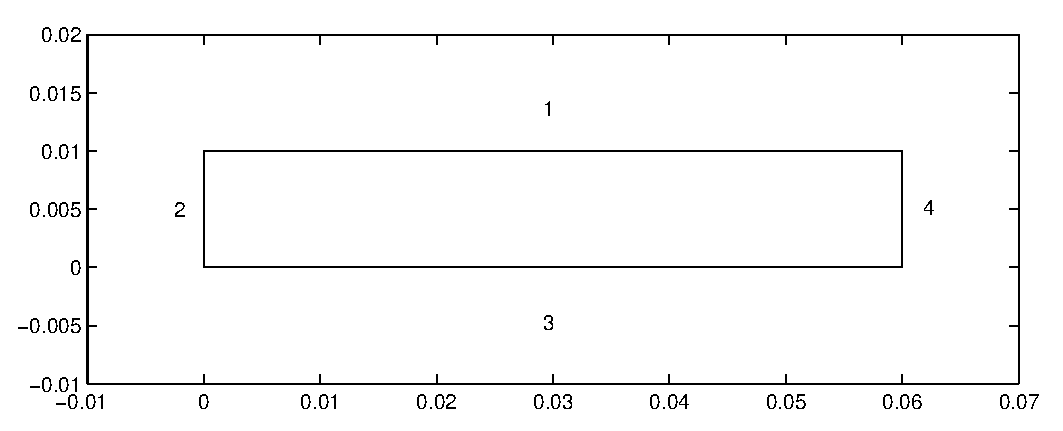
\includegraphics[width=150 mm, height=55 mm]{rb_geometry}
\caption{Domain.}\label{fg:rb_geometry}
\end{figure}  


\begin{table}[h]
\caption{Material parameters for water}
\label{tb:matpar}
\begin{center}
\begin{tabular}{ll} \hline
parameter  & value \\ \hline
density & 998.3 kg/m$^{3}$ \\
viscosity & 1040e-6 Ns/m$^{2}$ \\
heat capacity & 4183 J/(kg$\cdot$K) \\
heat conductivity & 0.58 W/(m$\cdot$K)       \\
heat expansion coefficient & 2.07e-4 K$^{-1}$      \\ 
reference temperature & 293 K       \\ \hline
\end{tabular}
\end{center}
\end{table}


\subsection*{Solution procedure}

The mesh is given in ElmerGrid format in file \texttt{rectangle.grd}, load this file.
\ttbegin
File 
  Open -> rectangle.grd
\ttend
You should obtain your mesh and may check \texttt{Model Summary...} that it consists 
of 3036 bilinear elements.  The geometry and mesh should look like 
figure \ref{fg:rb_geometry}.

There is a possibility to divide and unify edges to simplify the case definition in the future.
\ttbegin
Choose (left wall + right wall (Ctrl down)) -> unify edge
\ttend

After we have the mesh we start to go through the Model menu from the top to bottom. 
In the Setup we choose things related to the whole simulation such as file names, 
time stepping, constants etc.
The simulation is carried out in 2-dimensional Cartesian
coordinates. 2nd order bdf time stepping method is selected with 200 steps
and with step size of two seconds.
Gravity is needed for the buoyancy force and it is defined by a vector with four components. 
The first three components define a unit vector and the fourth its magnitude. 
\ttbegin
Model
  Setup 
    Simulation Type = Transient
    Steady state max. iter = 20
    Time Stepping Method = bdf
    BDF Order = 2
    Time Step Intervals = 200
    Time Step Sizes = 2.0
    Gravity = 0 -1 0 9.82
\ttend
In the equation section we choose the relevant equations and parameters related to their solution. 
In this case we'll have one set of equations (named ``Natural Convection'') which 
consists of the heat equation and of the Navier-Stokes equation.

When defining Equations and Materials it is possible to assign to the bodies immediately, or to use mouse
selection to assign them later. In this case we have just one body and therefore its easier to assign 
the Equation and Material to it directly.
It is important to select the 
convection to be computed since that couples the velocity field to the heat equation.

The system may include non-linear iterations of each equation and steady state iterations 
to obtain convergence of the coupled system. It is often a good idea to keep the number of 
non-linear iterations in a coupled case low. Here we select just one non-linear iteration
for both equations.

For the linear system solvers we are happy to use the defaults. One may however, try out different
preconditioners (ILU1,\ldots) or direct Umfpack solver, for example.
\ttbegin
Model
  Equation
    Name = Natural Convection
    Apply to Bodies = 1
    Heat Equation
      Active = on
      Convection = Computed
      Edit Solver Setting
        Nonlinear System
          Max. iterations = 1
    Navier-Stokes 
      Active = on
      Edit Solver Setting
        Nonlinear System
          Max. iterations = 1
    Add 
    OK
\ttend        
The Material section includes all the material parameters.
They are divided into generic parameters which are direct properties of the material
without making any assumptions on the physical model, such as the mass. Other properties assume
a physical law, such as conductivities and viscosity. 

Here we choose water at room temperature from the Material Library.
You may click through the material parameters of the various solvers to ensure that
the properties are indeed as they should be. Any consistent set of units may be used in Elmer.
The natural choice is of course to perform the computations in SI units. 

Apart from the properties from the material database, we enter a
reference temperature for the Boussinesq approximation.    

\ttbegin
Model
  Material
    Apply to Bodies = 1 
    Material library    
      Water (room temperature)
    General 
      Reference Temperature = 293
    Add
    OK
\ttend

A Body Force represents the right-hand-side of a equation. It is generally 
not a required field for a body. In this case, however, we apply the buoyancy resulting from
heat expansion as a body force to the Navier-Stokes equation.
\ttbegin
Model
  Body Force
    Name = Buoyancy
    Apply to Bodies = 1
    Navier-Stokes
      Boussinesq = on
    Add 
    OK
\ttend    

Initial conditions should be given to transient cases. In this case we choose a 
constant Temperature field and an small initial velocity that initializes the symmetry break. 
\ttbegin
Model
  Initial Condition 
    Name = Initial Guess
    Heat Equation
      Temperature = 293
    Navier-Stokes
      Velocity 1 = 1.0e-9
      Velocity 2 = 0.0
\ttend

Only one boundary condition may be applied to each boundary and therefore all the 
different physical BCs for a boundary should be grouped together. In this case the
Temperature and Velocity. The side walls are assumed to be adiabatic.
\ttbegin
Model
  BoundaryCondition
    Name = Bottom
    Heat Equation
      Temperature = 293.5
    Navier-Stokes 
      Velocity 1 = 0.0
      Velocity 2 = 0.0
    Add
    New

    Name = Top
    Heat Equation
      Temperature = 293
    Navier-Stokes 
      Velocity 1 = 0.0
      Velocity 2 = 0.0
    Add 
    New
 
    Name = Sides
    Navier-Stokes 
      Velocity 1 = 0.0
      Velocity 2 = 0.0
    Add
\ttend   

The conditions may also be assigned to boundaries in the Boundary condition menu, or 
by clicking with the mouse. Here we use the latter approach as that spares us of the 
need to know the indexes of each boundary.
\ttbegin
Model
  Set boundary properties
    Choose Bottom -> set boundary condition Bottom
    Choose Top -> set boundary condition Top
    Choose Sides -> set boundary condition Sides
\ttend

For the execution ElmerSolver needs the mesh files and the command file. 
We have now basically defined all the information for ElmerGUI to write 
the command file. After writing it we may also visually inspect the command file.
\ttbegin
Sif 
  Generate
  Edit -> look how your command file came out  
\ttend

Before we can execute the solver we should save the files in a directory. 
The ElmerGUI project includes all the files needed to restart the case.
\ttbegin
File 
  Save Project
\ttend

After we have successfully saved the files we may start the solver
\ttbegin
Run
  Start solver
\ttend
A convergence view automatically pops up showing relative changes of each iteration.

When there are some results to view we may start the postprocessor also
\ttbegin
Run
  Start ParaView
\ttend


\subsection*{Results}

Due to the number of the time steps the simulation may take around ten minutes.
You may inspect the results with Paraview as the time steps are computed, or
wait until all time steps have been computed. You must reload the files if their number has changed. 
The time series can be automatically animated and even saved to an animation file.

In Figures \ref{fg:rb_temp}  through \ref{fg:rb_velo} the obtained temperature 
and  velocity distribution are presented.  The maximum velocity in the system 
should be about 0.516~mm/s. 

\begin{figure}[h]
\centering
\includegraphics[width=150mm]{rb_temp}
\caption{Temperature distribution}\label{fg:rb_temp}
\end{figure} 

\begin{figure}[h]
\centering
\includegraphics[width=150mm]{rb_velo}
\caption{Velocity magnitudes}\label{fg:rb_velo}
\end{figure} 


\newpage

\subsection*{Extra task: Sensitivity to temperature difference}

If you have time you may try to solve the case with different parameters. Changing the temperature difference
is one way of affecting the instability of the system. Decreasing the temperature differences the system eventually becomes 
steady state and the convection rolls vanish altogether. Increasing the temperature difference may increase the 
number of convection rolls and eventually the system becomes fully chaotic. 
Note that changing the temperature difference also affects to the time scale of the wake. 

\hfill


% ElasticPlateLinear has been converted to ElmerGUI
%\graphicspath{{./}{ElasticPlateLinear/}}
%\chapter{Elastic linear plate}

\modinfo{Directory}{ElasticPlateLinear}
\modinfo{Solvers}{\Idx{SmitcSolver}}
\modinfo{Tools}{\Idx{ElmerGrid}, editor}
\modinfo{Dimensions}{2D}

\subsection*{Case definition}

This tutorial demonstrates how to use the Smitc solver to solve
small deflections of plates.
The Smitc solver is for elastic linear plates and
uses the theory of Reissner and Mindlin.

The case under investigation is a L-shaped steel plate under pressure.
The plate is shown in figure~\ref{fig:simplePlate}
The longer sides have the length of $2\,m$ and the shorter $1\,m$. 
So the area of the plate is $3\,m^2$. The plate has a thickness of
$1\,cm$. We assume that on the plate
there is about $15300\,kg$ of sand. The sand is uniformly distributed
on the plate and the sand stays uniformly distributed even if the 
plate undergoes small deflection. The sand exerts to the plate
a pressure of $50000\,Pa$. The plate is clamped from all sides
meaning that both deflection and rotation are zero on all edges.
%
\begin{figure}[tbhp]
\begin{center}
\includegraphics[width=0.4\textwidth]{simplePlate}
\end{center}
\caption{The geometry of plate and the numbering of edges.}
\label{fig:simplePlate}
\end{figure}

\subsection*{Solution Procedure}

The first thing to do is create a mesh with ElmerGrid.
The definition of mesh is in the file \texttt{simple\_plate.grd}.
The mesh is about uniform and consist of 1000 linear square elements.
The mesh is created with command
\ttbegin
ElmerGrid 1 2 simple_plate
\ttend
One thousand element should easily do the trick in this case
but if more elements is needed you can edit the file 
\texttt{simple\_plate.grd}.
More specifically the line
\ttbegin
Surface Elements = 1000
\ttend

The solver input file \texttt{simple\_plate.sif} starts with turning on 
the warnings and the definition of the proper mesh directory. 
%
\ttbegin
check keywords warn

Header
  Mesh DB "." "simple_plate"
End
\ttend
The simulation uses 2D cartesian geometry. The simulation is not
time dependent i.e. Steady State. 
There is no coupled solvers so only one iteration is needed. 
The output interval is one meaning all intervals (now there is only one
interval). Numerical results are written to file \texttt{simple\_plate.result}
and ElmerPost file is \texttt{simple\_plate.vtu}.
\ttbegin
Simulation
  Coordinate System = Cartesian 2D
  Simulation Type = Steady State
  Steady State Max Iterations = 1
  Output Intervals = 1
  Output File = "simple_plate.result"
  Post File = "simple_plate.vtu"
End
\ttend
There is just one body, the plate, and it uses Equation and  Body Force 1 and
is of Material 1.
\ttbegin
Body 1
  Equation = 1
  Body Force = 1
  Material = 1
End
\ttend
The equation block is now more than easy. 
It only states that we use Solver 1 to solve the equation.
\ttbegin
Equation 1
  Active Solvers(1) = 1
End
\ttend
In Body Force block we give the equations right hand side. 
It is the sands pressure and it is the same constant in every point.
\ttbegin
Body Force 1
  Pressure = 5.0e4
End
\ttend
In Material block we define the plates properties i.e. Poisson ratio,
Young's modulus and density. We also give the plates thickness and
possible pretension. Now there is no pretension.
\ttbegin
Material 1   
  Poisson ratio = 0.3
  Youngs modulus = 209e9
  Density = 7800.0

  Thickness = 1.0e-2
  Tension = 0.0
End
\ttend
Next the Solver block.
\begin{itemize}
\item First we define that we use SmitcSolver  
and give the name of the subroutine file \texttt{Smitc} and
subroutine name \texttt{SmitcSolver}. 
\item We name the variable Deflection and state that it has 3 degrees of freedom. 
First degree is the deflection and the remaining two are actually 
the components of rotation vector. 
\item We don't need eigen analysis nor is there any holes in the plate. 
\item We solve the matrix equation iteratively with stabilized biconjugate 
gradient method. We precondition the iteration with incomplete 
LU-factorization. 
\item Tolerance for the matrix system is $1\cdot10^{-8}$
and the tolerance should be achieved in less than 300 iteration.
\end{itemize}
\ttbegin
Solver 1
  Equation = "SmitcSolver"
  Procedure = "Smitc" "SmitcSolver"

  Variable = Deflection
  Variable DOFs = 3

  Eigen Analysis = False
  Hole Correction = False

  Linear System Solver = Iterative
  Linear System Iterative Method = BiCGStab
  Linear System Preconditioning = ILU2
  Linear System Convergence Tolerance = 1.0e-8
  Linear System Max Iterations = 300
End
\ttend
Finally we give the boundary conditions. The plate has 6 edges and
the edge numbering is in figure~\ref{fig:simplePlate}. All the edges are
clamped i.e. no deflection (Deflection 1) and  no rotation (Deflection 2 and 3).
\ttbegin
Boundary Condition 1
  Target Boundaries(6) = 1 2 3 4 5 6
  Deflection 1 = 0.0
  Deflection 2 = 0.0
  Deflection 3 = 0.0
End
\ttend

\subsection*{Results}

The problem is solved in few seconds and the results are viewed historically with ElmerPost. Currently you would use Paraview or something that can read the
VTU files. Here the results are still shown as originally done in ElmerPost.

Note that the 1st component of Deflection is the displacement to normal
direction whereas the 2nd and 3rd components are the x- and y-components of
rotation vector.

Result is shown in figure~\ref{fig:simplePlateDeflection}.
%
\begin{figure}[tbhp]
\begin{center}
\includegraphics[width=0.48\textwidth]{simplePlateDeflection}
\includegraphics[width=0.48\textwidth]{simplePlateRotation}
\end{center}
\caption{The deflection of the plate and the corresponding rotation.}
\label{fig:simplePlateDeflection}
\end{figure}
%
%\begin{figure}[tbhp]
%\begin{center}
%\includegraphics[width=0.5\textwidth]{simplePlateRotation}
%\end{center}
%\caption{The rotation of the plate.}
%\label{fig:simplePlateRotation}
%\end{figure}



% Radiation example has been converted to ElmerGUI
%\graphicspath{{./}{TemperatureRadiation/}}
%\chapter{Heat Equation -- 2D -- Axi Symmetric Steady State Radiation}

\modinfo{Directory}{Radiation}
\modinfo{Solvers}{\Idx{HeatSolve}}
\modinfo{Tools}{\Idx{ElmerGUI}}
\modinfo{Dimensions}{2D, Axi-Symmetric}
\modinfo{Author}{not listed in original}


\subsection*{Case definition}

At high temperature the radiation heat transfer between walls 
is often the dominating heat transfer mechanism. In this
tutorial we examine how radiation heat transfer between 
concentric cylinders is modelled.\\

The problem is a pure heat transfer problem that may be solved
with \texttt{HeatSolve}. The view and Gebhart factors 
associated with the radiation are solved as a first step 
in solving the equations. Thereafter the non-linear heat equation 
is solved until convergence is reached.


\begin{figure}
\begin{center}
\includegraphics[width=100 mm]{geometry}
\caption{Geometry and mesh}\label{fg:geometry}
\end{center}
\end{figure}  


\subsection*{Solution procedure}

The mesh is given in ElmerGrid format in file \texttt{radiation.grd}, load this file.
\ttbegin
File 
  Open -> radiation.grd
\ttend
You should obtain your mesh and may check \texttt{Model Summary...} that 
it consists of 1231 surface elements.  Your geometry and mesh should look something
like as shown in figure \ref{fg:geometry}\\


After we have the mesh we start to go through the Model menu from the top to bottom. 
In the Setup we choose things related to the whole simulation such as file names, 
time stepping, constants etc.  

The simulation is carried out in Axi Symmetric coordinates. The only constant 
required is the Stefan-Boltzmann constant that gives the
relationship between temperature and radiation power, and this
constant is predefined in the \texttt{Setup} menu.

\ttbegin
Model
  Setup 
     Coordinate System = Axi Symmetric
     Simulation Type = Steady State
     Steady State Max Iterations = 1
     Output Intervals = 1
  Apply
\ttend
In the equation section we choose the relevant equations and parameters related to their solution. 
In this case we'll have the Heat equation.

When defining Equations and Materials it is possible to assign to the bodies 
immediately, or to use mouse selection to assign them later. In this case we 
have just two bodies and therefore its easier to assign the Equation and 
Material to it directly.

For the linear system solvers we are happy to use the defaults. One may however, try out different
preconditioners (ILU1,\ldots) or direct Umfpack solver, for example.
\ttbegin
Model
  Equation
   Name = Radiation
    Apply to Bodies = 1 2
    Heat Equation
      Active = on
    Edit Solver Settings
       Steady State
         Convergence Tolerance = 1.0e-8
       Non-linear system
        Convergence Tolerance = 1.0e-8
        Max Iterations = 50
        Relaxation Factor = 0.7
        Newton After Iterations = 1
        Newton After Tolerance = 1.0e-4
      Linear system
        Convergence Tolerance = 1.0e-12
        Preconditioning = ILU1
    Add 
    OK
\ttend        
The Material section includes all the material parameters. They are divided into 
generic parameters which are direct properties of the material without making 
any assumptions on the physical model, such as the mass. Other properties 
assume a physical law, such as conductivities and viscosity. 

The material properties differ only in heat conductivity. Heat capacity is not
actually needed since the case is not transient. The inner body has ten times
higher conductivity than the outer body.

\ttbegin
Model
  Material
    Name = Inner
    Apply to Bodies = 1 
    General 
      Density = 1.0
      Heat capacity = 1.0
    Heat Equation
      Heat Conductivity = 10.0
    Add
    New

    Name = Outer
    Apply to Bodies = 2 
    General 
      Density = 1.0
      Heat capacity = 1.0
    Heat Equation
      Heat Conductivity = 1.0
    Add
    OK
\ttend

A Body Force represents the right-hand-side of a equation. The body 
force is the heating power in units W/kg. 
 

\ttbegin
Model
  Body Force
    Name = Power
    Apply to Bodies = 1
    Heat Equation
       Volume Heat Source = 10000
    Add 
    OK
\ttend    

Initial conditions are needed in this case. We choose a 
constant Temperature field of 250C. 
\ttbegin
Model
  Initial Condition 
    Name = Initial
    Apply to Bodies = 1 2
    Heat Equation
      Temperature = 250.0
    Add 
    OK
\ttend

Only one boundary condition may be applied to each boundary and therefore all the 
different physical BCs for a boundary should be grouped together. 

The radiation boundary conditions are set for two different boundaries. The first one
is for the internal heated object and the second one for the outer insulating body. 
The normal direction of the surfaces is important since a wrong direction may 
result to a badly set problem for the view factor computation. Internal and 
external surfaces are very different.  The normal direction may be switched 
with the input box \texttt{Radiation Target Body}. A good sign of a properly 
set case is that the view factors add up to about one.

The third boundary condition is the Dirichtlet condition for the external boundary.
Dirichtlet conditions boost up the convergence even though the heat equation 
is basically well defined also with external radiation conditions.
\ttbegin
Model
  BoundaryCondition
    Name = Inner
    Apply to Bodies = 1
    Heat Equation
      Radiation Settings = Diffuse Gray
      Emissivity = 0.6
      Radiation Target Body = -1
    Add
    New

    Name = Outer
    Apply to Bodies = 2
    Heat Equation
      Radiation Settings = Diffuse Gray
      Emissivity = 0.1
      Radiation Target Body = -1
    Add 
    New

    Name = Exterior
    Apply to Bodies = 3
    Heat Equation
      Temperature = 100.0
    Add 
    OK
\ttend   

The conditions may also be assigned to boundaries in the Boundary condition menu, or 
by clicking with the mouse. Here we use the latter approach as that spares us of the 
need to know the indexes of each boundary.
\ttbegin
Model
  Set boundary properties
   Choose Inner -> set boundary condition Inner
   Choose Outer -> set boundary condition Outer
   Choose Exterior -> set boundary condition Exterior
  Update
\ttend


For the execution ElmerSolver needs the mesh files and the command file. 
We have now basically defined all the information for ElmerGUI to write the 
command file. After writing it we may also visually inspect the command file.
\ttbegin
Sif 
  Generate
  Edit -> look how your command file came out  
\ttend

Before we can execute the solver we should save the files in a directory. 
The ElmerGUI project includes all the files needed to restart the case.
\ttbegin
File 
  Save Project
\ttend

After we have successfully saved the files we may start the solver
\ttbegin
Run
  Start solver
\ttend
A convergence view automatically pops up showing relative changes of each iteration.

When there are some results to view we may start the postprocessor also
\ttbegin
Run
  Start ParaView
\ttend

\subsection*{Results}

With the given computational mesh the problem is solved in 
a few seconds. With 1,231 second order 9-noded
rectangular elements the maximum temperature is 565.7~K.
The corresponding results are shown in Fig.~\ref{fig:temp_rad1}.

\begin{figure}
\begin{center}
  \includegraphics[width=100mm]{temp_rad1}
\end{center}
\caption{Temperature distribution in the radiation heat transfer
problem}
\label{fig:temp_rad1}
\end{figure}
 



\hfill


% FlowStepCompressible example has been converted to ElmerGUI
%\graphicspath{{./}{FlowStepCompressible/}}
%\chapter{Compressible flow passing a step}

\modinfo{Directory}{FlowStepCompressible}
\modinfo{Solvers}{\Idx{FlowSolve}, \Idx{HeatSolve}}
\modinfo{Tools}{\Idx{ElmerGrid}, Editor}
\modinfo{Dimensions}{2D, Steady-state}

\subsection*{Case definition}

This tutorial demonstrates how to simulate compressible air flowing past a step. The whole step has length of 1.4 m and the height of 0.2 m and the first part of it has length of 0.4 m and the height of 0.1 m (Figure \ref{fg:step_geometry}). The needed material parameters of air are shown in Table \ref{tb:matpam}. 
The model has three sets of boundary conditions.
The air flows into the step from the inlet region and withdraws from the outlet region. The other edges of the step compose the third boundary. The flowing air is considered as an ideal gas in this case, and its density $\rho$  depends on the pressure $p$ and temperature $T$ through the equation of state
\begin{displaymath}
\rho = \frac{p}{RT},
\end{displaymath}
where $R$ is the gas constant.

\begin{figure}[h]
\centering
\includegraphics[height=80mm]{step_geometry.png}
\caption{Step.}\label{fg:step_geometry}
\end{figure}

\begin{table}[h]
\caption{Material parameters.}
\label{tb:matpam}
\begin{center}
\begin{tabular}{ll} \hline
parameter  & value \\ \hline
viscosity & 16.7e-6 Ns/m$^{2}$  \\
heat conductivity & 0.026 W/(m$\cdot$K) \\
heat capacity & 1.01e3 J/(kg$\cdot$K) \\
specific heat ratio & 1.4        \\
reference pressure & 1e5 Pa      \\ \hline
\end{tabular}
\end{center}
\end{table}


\subsection*{Solution procedure}

\begin{flushleft}

The mesh consists of 500 rectangular elements and it is constructed using ElmerGrid with the following command

\ttbegin
ElmerGrid 1 2 mesh.grd
\ttend

This command creates the sub-directory {\tt mesh} which contains the Elmer mesh files.

\ttbegin
Header
  Mesh DB "." "mesh"
  Include Path ""
  Results Directory ""
End
\ttend

The simulation uses 2D Cartesian geometry and the problem is solved in steady state using no more than twenty steady state iterations.

\ttbegin
Simulation
  Coordinate System =  Cartesian 2D
  Coordinate Mapping(3) = 1 2 3
  Simulation Type = Steady
  Steady State Max Iterations = 20
  Solver Input File = "compress_step.sif"
  Post File = "compress_step.vtu"
  Output File = "compress_step.dat"
End
\ttend

The solvers are coupled and therefore the convection is computed. 

\ttbegin
Equation 1
  Navier-Stokes = True
  Heat Equation = True
  Convection = "Computed"
End
\ttend

Due to the simplicity of the model only one body is needed.

\ttbegin
Body 1
  Equation = 1
  Material = 1
  Initial Condition = 1
End
\ttend

Our intention is to model compressible flow and that is why we have to set the value ''Perfect Gas'' for the keyword {\tt Compressibility Model}. Furthermore, because perfect gas model has been chosen the settings {\tt Reference Pressure} and {\tt Specific Heat Ratio} must also be given. The Navier-Stokes equation also needs the value of viscosity and the heat equation needs the values of heat capacity and heat conductivity.

\ttbegin
Material 1
  Compressibility Model = String "Perfect Gas"
  Reference Pressure = 1e5
  Specific Heat Ratio = 1.4
  Viscosity = 16.7e-6
  Heat Conductivity = 0.026
  Heat Capacity = 1.01e3
End
\ttend

For the initial value of temperature we have chosen 300 K.

\ttbegin
Initial Condition 1
  Temperature = 300
End
\ttend

The Navier-Stokes equation is solved first. Here we give the linear system solver and convergence criterions for linear, nonlinear and steady state solution of the Navier-stokes equation. Note that we are solving for the compressible Navier-stokes equation and that is why a bubble function formulation is used for stabilization of the equation.


\ttbegin
Solver 1
  Equation = "Navier-Stokes"
  Linear System Solver = "Iterative"
  Linear System Iterative Method = "BiCGStab"
  Linear System Max Iterations = 500
  Linear System Convergence Tolerance = 1.0e-08
  Linear System Abort Not Converged = True
  Linear System Preconditioning = "ILU2"
  Linear System Residual Output = 1
  Steady State Convergence Tolerance = 1.0e-05
  Bubbles = Logical True
  Nonlinear System Convergence Tolerance = 1.0e-05
  Nonlinear System Max Iterations = 1
  Nonlinear System Newton After Iterations = 3
  Nonlinear System Newton After Tolerance = 1.0e-02
  Nonlinear System Relaxation Factor = 1
End
\ttend

The corresponding parameters for the solver of the heat equation are defined in the following solver section.

\ttbegin
Solver 2
  Equation = "Heat Equation"
  Variable = "Temperature"
  Linear System Solver = "Iterative"
  Linear System Iterative Method = "BiCGStab"
  Linear System Max Iterations = 350
  Linear System Convergence Tolerance = 1.0e-08
  Linear System Preconditioning = "ILU0"
  Linear System Residual Output = 1
  Steady State Convergence Tolerance = 1.0e-05
  Bubbles = Logical True
  Nonlinear System Convergence Tolerance = 1.0e-05
  Nonlinear System Max Iterations = 1
  Nonlinear System Newton After Iterations = 3
  Nonlinear System Newton After Tolerance = 1.0e-02
  Nonlinear System Relaxation Factor = 1
End
\ttend

Finally, the boundary conditions are specified. There are three sets of boundary conditions, so three {\tt Boundary Condition} sections are needed. The first one is used to prescribe the boundary conditions in the inlet region. Note that we have defined the x-velocity and temperature as a variable of y-coordinate. 
This is done by setting different values for the x-velocity and temperature 
(the numerical values of the second column between the words {\tt Real} and {\tt End})
in the different y-points
(the numerical values of the first column between words {\tt Real} and {\tt End})
of the inlet region.
This kind of procedure prevents singularities from occurring in the corner points of the inlet region. In addition, this kind of definition is more realistic than a constant condition, in which the values of the x-velocity and temperature remain the same in the whole inlet region. 

\ttbegin
Boundary Condition 1
  Target Boundaries = 1
  Velocity 1 = Variable Coordinate 2
    Real 
      0.1    0
      0.15   0.02
      0.2    0
    End

  Velocity 2 = 0
  Temperature = Variable Coordinate 2
    Real 
      0.1    300
      0.15   350
      0.2    300
    End
End
\ttend

After the rest of the boundary conditions have been defined the problem is ready to solve.

\ttbegin
Boundary Condition 2
  Target Boundaries = 2
  Velocity 2 = 0
End

Boundary Condition 3
  Target Boundaries = 3
  Velocity 1 = 0
  Velocity 2 = 0
  Temperature = 300
End
\ttend

\subsection*{Results}

Figure \ref{fg:comp_step_temp} presents the temperature distribution of the step in steady state. The maximum and minimum values of x- and y-velocities are also given as a result and they are shown in Table \ref{tb:velocities}.

\begin{figure}[h]
\centering
\includegraphics[height=80mm]{comp_step_temp.png}
\caption{Step.}\label{fg:comp_step_temp}
\end{figure}

\begin{table}[h]
\caption{Computed velocities.}
\label{tb:velocities}
\begin{center}
\begin{tabular}{ll} \hline
velocity  & value \\ \hline
min x-velocity & -0.0014 m/s\\
min y-velocity & -0.0016 m/s        \\
max y-velocity & 0.0008 m/s      \\ \hline
\end{tabular}
\end{center}
\end{table}

\end{flushleft}

\vfill


% Acoustic Waves has been converted to ElmerGUI
%\graphicspath{{./}{AcousticWaves/}}
%\chapter{Lossless \Idx{acoustic waves}}

\modinfo{Directory}{AcousticWaves}
\modinfo{Solvers}{\Idx{HelmholtzSolve}} 
\modinfo{Tools}{\Idx{ElmerFront}} 
\modinfo{Dimensions}{2D, Harmonic}


\subsection*{Introduction}

Note: this case cannot be performed as of today since ElmerFront is
since long obsolite. To mimic the ideas look at files domain.grd and
helmholtz-new.sif to try to do the case without ElmerFront.

To run the updated case just say:
\ttbegin
ElmerGrid 1 2 domain.grd
ElmerSolver helmholtz-new.sif
\ttend

Elmer provides two alternative ways of conducting acoustic analyses in the
frequency domain. Firstly, one may simply use the Helmholtz equation which 
is based on the assumption of lossless flow, i.e.\ the effects of viscosity 
and heat conduction are assumed to be negligible. More refined analyses where 
these effects are taken into account may be carried out by using the specific 
solver for the set of time-harmonic dissipative acoustic equations. 
The aim of this tutorial is to demonstrate the usage of the solver
for the basic Helmholtz equation, which is frequently taken as the starting
point in acoustic analyses. 

\subsection*{Case description}

In this problem the fluctuations of the pressure in an air-filled
cavity shown in Figure~\ref{cavity.fig} are considered. The cavity is 
connected with the surrounding air by an open narrow pipe. The pressure 
fluctuations are generated by a vibrating membrane on the boundary $\Gamma_S$ 
with the frequency of the motion being $f=100$ Hz. 
The remaining parts of the boundary are assumed to be rigid walls. 
In addition, the effects of gravity are assumed to be negligible.

\begin{figure}
\setlength{\unitlength}{1mm}
\begin{center}
\begin{picture}(60,50)(0,-10)
\put(0,0){\line(1,0){50}}
\put(0,0){\line(0,1){30}}
\put(0,30){\line(1,0){21}}
\put(29,30){\line(1,0){21}}
\put(29,30){\line(0,1){10}}
\put(21,30){\line(0,1){10}}
\put(21,40){\line(1,0){8}}
\put(50,0){\line(0,1){30}}
\put(25,-1){\line(0,1){2}}
\put(40,-1){\line(0,1){2}}
\put(31,2){$\Gamma_S$}
\put(23,42){$\Gamma_0$}
\put(55,15){\vector(0,1){15}}
\put(55,15){\vector(0,-1){15}}
\put(55,35){\vector(0,1){5}}
\put(55,35){\vector(0,-1){5}}
\put(15,-5){\vector(-1,0){15}}
\put(15,-5){\vector(1,0){10}}
\put(33,-5){\vector(-1,0){8}}
\put(33,-5){\vector(1,0){7}}
\put(45,-5){\vector(-1,0){5}}
\put(45,-5){\vector(1,0){5}}
\put(15,22){\vector(-1,0){15}}
\put(15,22){\vector(1,0){6}}
\put(25,22){\vector(-1,0){4}}
\put(25,22){\vector(1,0){4}}
\put(10,-4){0.25}
\put(30,-4){0.15}
\put(43,-4){0.1}
\put(57,14){0.3}
\put(57,34){0.1}
\put(10,23){0.3}
\put(22,23){0.08}
\end{picture}
\end{center}
\caption{The geometry of the cavity.}
\label{cavity.fig}
\end{figure}

Suitable boundary conditions in terms of the pressure must be given. 
On the rigid walls the pressure flux is prescribed to vanish which 
corresponds to the assumption that there is no velocity in the direction 
normal to the boundary. At the open end $\Gamma_0$ the impedance boundary 
condition suitable for forward traveling plane waves is given by setting 
$Z=-c$ with $c$ being the sound speed. We assume that $c=343$ (m/s). 
Finally, the wave source is given by defining a non-vanishing pressure
flux on the corresponding part of the boundary. We take simply 
$\nabla P \cdot \vec n = 1$ where $P$ is the (complex)
amplitude of the pressure and $\vec n$ is the outward unit normal to the
boundary. 


\subsection*{Solution procedure}

\begin{itemize}

\item Before starting Elmer copy the geometry file ({\tt domain.egf}) to the 
working directory and then launch Elmer Front by giving the command
\ttbegin
ElmerFront
\ttend 

\item Open the geometry file by choosing Open Cad-file in the  
File menu. To enable browsing with the mouse click the button on the 
right-hand side of the field where the file name may be written. Here
the correct Cad file type is Elmer. Give also the model name (for example
{\tt helmholtz}) and write the path of the working directory in the
Model directory field.  

\item Select the equation to be solved by selecting Equations in
the Problem menu. Choose the Helmholtz equation and press 
{\tt Add} button. 

\item Define the angular frequency for the simulation by selecting 
Simulation parameters in the Problem menu. Enter the value
628.3 to the field and accept the value by clicking {\tt OK} button.

\item Define the sound speed for the medium by selecting 
Materials in the Model menu. Enter the value
343 for the sound speed and press {\tt Add} button.

\item Prescribe the boundary conditions by selecting 
Boundary conditions in the Model menu. Select (with the mouse)
Boundary1 and give the value for the boundary flux: 
\ttbegin
Wave flux Re = 1
Wave flux Re = 0
\ttend 
Finally, press {\tt Add} button. Then proceed to give 
the other boundary conditions in a similar manner (the value for the 
pressure is prescribed).

\item Create a finite element mesh  by selecting 
Define mesh in the Mesh menu. To begin with give a name for the mesh.
Define the number of element
edges on each boundary and then create the mesh by pressing
{\tt Generate Mesh} button.   

\item The problem may now be solved by selecting Solver in the Run menu.

\item After the solution is done, view the results by selecting the
Postprocessor from the Run menu.
\ttbegin
Run -> Postprocessor
\ttend
\item To save the created model, select Save model file from the File menu.
\ttbegin
File -> Save model file
\ttend
\end{itemize}


   

\subsection*{Results}

Using a mesh consisting of 3900 (quadratic) elements with 7601 nodes
the difference of the maximum and the minimum value of the pressure 
is found to be $\Delta p \approx 0.205$


   























% Passive Elements has been converted to ElmerGUI
%\graphicspath{{./}{PassiveElements/}}
%\chapter{Active and passive elements}

\modinfo{Directory}{PassiveElements}
\modinfo{Solvers}{\Idx{HeatSolve}}
\modinfo{Tools}{\Idx{ElmerGrid}, editor}
\modinfo{Dimensions}{2D}

\subsection*{Case definition}

This tutorial shows an example of using \Idx{passive elements} in
Elmer. This feature allows the activation and deactivation of
parts of the geometry during the simulation. This tutorial uses the
heat equation solver to demonstrate this capability. Use with other
solvers is analogous.

The geometry of the problem consists of two parts. The lower edge of
the lower part is held at constant temperature of 1 degrees. The upper
body is heated with a constant heating power. Between time steps 5 and
6 the two bodies are connected by two heat conductors, and the heat is
conducted from the higher body to the lower one. The goal of the
simulation is to model the temperature distribution in the system over
time. 

The problem is a pure heat transfer problem that may be solved
with \texttt{HeatSolve}. 


\subsection*{Solution Procedure}

The computational mesh is done with \texttt{ElmerGrid} in directory \texttt{tmesh} 
with the command 
%
\ttbegin
ElmerGrid 1 2 tmesh
\ttend
%
The command file may be written with a text editor. The file includes
the following information. 

The mesh directory is given in the header of the command file
%
\ttbegin
Header
  Mesh DB "." "tmesh"
End
\ttend
%
The simulation block of the command file defines, eg., the case to be time
dependent (transient) with 1 second time steps and altogether 15 time
intervals.  
%
\ttbegin
Simulation
  Max Output Level = 32
  Coordinate System = Cartesian 2D
  Simulation Type = Transient
  Timestepping Method = BDF
  BDF Order = 2
  Timestep Intervals = 15
  Timestep Sizes = 1
  Output Intervals = 1
  Steady State Max Iterations = 1
  Output Version Numbers = Logical True
  Output File = heat.res
  Post File = heat.ep
End
\ttend
%
The heat equation solver asks for the Stefan-Boltzmann constant that
gives the relationship between temperature and radiation power,
although radiation is not needed here. Let us define it anyway to
avoid warnings of missing parameters.
%
\ttbegin
Constants
  Stefan Boltzmann = 5.67e-8
End
\ttend
%
There are three bodies with the same equation but different material
properties. Body 3 is heated by a constant body force. Body 2 forms
the connecting parts of the system. An initial condition as well as a
body force is defined for this body. The body force contains the
initial deactivation, and later activation, of the connecting
part. Note that this part is included in the geometry all the time,
but the command file is used to define when they are included into the
simulation.
%
\ttbegin
Body 1
  Equation = 1
  Material = 1
End

Body 2
  Equation = 1
  Material = 2
  Body Force = 2
  Initial Condition = 1
End

Body 3
  Equation = 1
  Material = 1
  Body Force = 1
End
\ttend
%
The only solver is the heat solver (Solver 1)
%
\ttbegin
Equation 1
  Active Solvers = 1
End
\ttend
%
The initial condition for the initially passive elements is taken to
be 1 degree; the same temperature than the colder part of the system
has as a boundary condition.
%
\ttbegin
Initial Condition 1
  Temperature = 1.0
End
\ttend
%
The heating power is defined to be 10 W/kg
%
\ttbegin
Body Force 1
  Heat Source = 10
End
\ttend
%
Now the passive condition for the connecting part is defined. When the
parameter \texttt{Temperature Passive} has a value larger than zero,
the current element is excluded from the solution, otherwise it is
included as a normal element. The parameter may depend on variables,
coordinates or time. Here it is defined to depend on time using a
tabular format.
%
\ttbegin
Body Force 2
  Temperature Passive = Variable Time
    Real
      0.0    1.0
      5.0    1.0
      5.2   -1.0
      8.0   -1.0
    End

End
\ttend
%
The material properties of the system are artificial. The following
three properties are needed for each material.
%
\ttbegin
Material 1
  Heat Capacity = 1
  Heat Conductivity = 1
  Density = 1
End

Material 2
  Heat Capacity = 10
  Heat Conductivity = 1
  Density = 1
End
\ttend
%
The heat equation is solved with an iterative method. The system is
linear, thus multiple non-linear iterations are not needed.
%
\ttbegin
Solver 1
  Equation = heat equation
  Linear System Solver = Iterative
  Linear System Iterative Method = BiCGStab
  Linear System Preconditioning = ILU0
  Linear System Max Iterations = 300
  Linear System Convergence Tolerance = 1.0e-6
  Linear System Abort Not Converged = Logical False
  Nonlinear System Max Iterations = 1
  Nonlinear System Convergence Tolerance = 1.0e-5
  Steady State Convergence Tolerance = 1.0e-5
End
\ttend
%
The boundary conditions are simple. The lower boundary of the lower
body is held at 1 degree and the upper boundary of the upper body at
10 degrees.
%
\ttbegin
Boundary Condition 1
  Target Boundaries = 1

  Temperature = 1
End

Boundary Condition 2
  Target Boundaries = 4

  Temperature = 10
End
\ttend

After writing the command file is finished, the problem can be solved
by entering the command \texttt{ElmerSolver} on the command line. The
results can be examined with \texttt{ElmerPost}.


\subsection*{Results}

\begin{figure}
\begin{center}
  \includegraphics[height=0.5\textwidth]{heat.png}
\end{center}
\caption{Temperature distribution of the system at the final time
  instant (with spectral\_32 color map).}
\label{fig:temp_passive}
\end{figure}
 
With the given computational mesh the problem is solved in a few
seconds. The maximum and minimum temperatures in the system over the
whole simulation are 15.466 degrees and 0.6525 degrees
respectively. The maximum and minimum temperature at the final time
instant are 14.207 degrees and 1.000 degrees, respectively.  The
results at the time instant of 15 seconds are shown in
Fig.~\ref{fig:temp_passive}.


\subsection*{Notes}

For equations with more than one components (such as displacement for
Stress Analysis solver in 2D or 3D) the passive elements feature apply
to all the components. The feature is activated by defining, eg.,
\texttt{Displacement Passive} in the Body Force section. Note that
for Navier-Stokes equations one should use \texttt{Flow Solution
  Passive}, and that this affects the Pressure as well as the Velocity
components. 

However, when using multiple solvers, one can define some of them
passive and some of them active at the same time.


\hfill

% Microfluidics has been converted to ElmerGUI and renamed to be Electrokinetics
%\graphicspath{{./}{Microfluidic/}}
%\chapter{Electroosmotic flow and advected species}

\modinfo{Directory}{Microfluidic}
\modinfo{Solvers}{\Idx{StatElecSolve}, \Idx{FlowSolve },
  \Idx{AdvectionDiffusion}, \Idx{Electrokinetics}}
\modinfo{Tools}{\Idx{ElmerGrid}, editor}
\modinfo{Dimensions}{2D}


\subsection*{Case definition}

This tutorial is an example of setting up a simulation for
(microfluidic) electroosmotic flow advecting a passive scalar
quantity. Diffusion of the species is also included. The geometry of
the system is a simple 2D microchannel with T crossing. The flow is
induced by the applied electric field and the electric double layer at
the channel walls. The analyte (species) is inserted into the system
from the left hand side inlet.

More details on the electrokinetic capabilities of Elmer are found on
the Models Manual, chapter ``Electrokinetics''.


\subsection*{Solution Procedure}

The computatonal mesh is done with \texttt{ElmerGrid} in directory
\texttt{Tcross} with the command 
%
\ttbegin
ElmerGrid 1 2 Tcross -scale 1e-5 1e-5 1e-5
\ttend
%
The scale option above is used to obtain appropriate dimensions from a
geometry template defined in nondimensional units.

The command file may be written with a text editor. The file includes
the following information. 

The mesh directory is given in the header of the command file
%
\ttbegin
Header
  Mesh DB "." "Tcross"
End
\ttend
%
The simulation block of the command file defines, eg., the case to be time
dependent (transient) with $10^{-5}$ second time steps and altogether
120 time intervals. Results from every second time step are saved into
the files \texttt{diffusion1.*}.
%
\ttbegin
Simulation
  Coordinate System = Cartesian 2D

  Simulation Type = "Transient"
  Steady State Max Iterations = 20

  Timestep Intervals = 120
  Timestep Sizes = 1e-5  
  Output Intervals = 2

  Timestepping Method = BDF
  BDF Order = 2

  Binary Output = Logical True

  Output File = "diffusion1.res"
  Post File = "diffusion1.ep"

  Output Version Numbers = Logical True
  Max Output Level = 32
End
\ttend
%
The electrostatics and electrokinetics solvers require the value of
the permittivity of vacuum. This is actually not even needed here
since the case deals with conducting media. Thus the value has been
fixed as 1.0 to avoid warnings on missing constant definitions.
%
\ttbegin
Constants
!  Permittivity Of Vacuum = 8.8542e-12  ! C\verb|^2|/Nm\verb*|^2|
  Permittivity Of Vacuum = 1.0 ! manipulation for conducting material
End
\ttend
%
The case includes only one body. The corresponding equation definitions are
found in section \texttt{Equation 1} and material parameters from
section \texttt{Material 1}.
%
\ttbegin
Body 1
  Equation = 1
  Material = 1
End
\ttend
%
All three solvers are active in this equation set. Further definitions
include, first, that the convection of the species is switched on
(besides diffusion). Then that for Navier-Stokes equations the
convective term may be left out resulting in laminar Stokes flow, and
finally that the electric field is computed by the electrostatics
rather than given by the user.
%
\ttbegin
Equation 1
  Active Solvers(3) = 1 2 3
  Convection = Computed
  NS Convect = False
  Electric Field = String "computed"
End
\ttend
%
Following are the solver definitions. Solver 1 is the electrostatics
solver. The equation is linear and thus no non-linear iterations are
needed. The equation is solved using a fast direct method UMFPack.
%
\ttbegin
Solver 1  
  Equation = "Stat Elec Solver"
  Procedure = "StatElecSolve" "StatElecSolver"
  Variable = String "Potential"
  Variable DOFs = 1

  Calculate Electric Field = True
  Calculate Electric Flux = False
  Linear System Convergence Tolerance = 1.0E-10

  Linear System Solver = Direct
  Linear System Direct Method = UMFPack 
  Linear System Preconditioning = ILU1
  Linear System Residual Output = 1

  Nonlinear System Max Iterations = 1
  Nonlinear System Convergence Tolerance = 1.0e-10
  Steady State Convergence Tolerance =  1.0E-10
End
\ttend
%
The next solver is for the Navier-Stokes equations. Here non-linear
iterations are required.
\ttbegin
Solver 2
  Equation = "Navier-Stokes"

  Linear System Convergence Tolerance = 1.0D-08
  Linear System Solver = Iterative
  Linear System Iterative Method = "BiCGStab"
  Linear System Max Iterations = 500
  Linear System Abort Not Converged = False  ! True
  Linear System Preconditioning = ILU1 
  Linear System Residual Output = 10  

  Nonlinear System Convergence Tolerance = 1.0e-6
  Nonlinear System Max Iterations = 30
  Nonlinear System Newton After Iterations = 10
  Nonlinear System Newton After Tolerance =  Real 1.0D-8
  Nonlinear System Relaxation Factor = 1.0
  Steady State Convergence Tolerance =  1.0D-03

  Stabilize = True
End
\ttend
%
The advection-diffusion equation does not affect either the
electrostatic field or the flow, thus it may be solved only after a
converged solution for the previous two equations is available. This
is achieved with the \texttt{Exec Solver} definition below. The
advected quantity is given the name Analyte.
The advection-diffusion solver uses bubble stabilization method to
avoid numerical problems associated with convection type equations.
%
\ttbegin
Solver 3
  Exec Solver = After Timestep
  Equation = "Analyte transfer"
  Procedure = "AdvectionDiffusion" "AdvectionDiffusionSolver"
  Variable = String "Analyte"
  Variable DOFs = 1

  Bubbles = True

  Linear System Convergence Tolerance = 1.0E-06
  Linear System Solver = "Iterative"
  Linear System Iterative Method = "BiCGStab"
  Linear System Max Iterations = 500
  Linear System Preconditioning = ILU2
  Linear System Residual Output = 1

  Nonlinear System Max Iterations = 1
  Nonlinear System Convergence Tolerance = 1.0e-5
  Steady State Convergence Tolerance =  1.0D-06
End
\ttend
%
The material parameters are given below.
%
\ttbegin
Material 1
  Density = 1e3  
  
  Viscosity = 1e-03

  Relative Permittivity = 1.0    !  this is actually electric conductivity

  Analyte Diffusivity = Real 1e-10 
End
\ttend
%
Finally the boundary conditions are defined. The first BC is given for
the channel walls. Here, tangential velocity (velocity components 1
and 2) is computed by the Helmholtz-Smoluchowski slip velocity
condition, which means that the velocity is computed using the
computed electric field and the electroosmotic mobility as inputs. 
%
\ttbegin
Boundary Condition 1
  Name = "channel-walls"
  Target Boundaries(2) = 4 5

  EO Mobility = Real 5e-08 

  Velocity 1 = Variable Pressure
      Real Procedure  "Electrokinetics" "helmholtz_smoluchowski1"
  Velocity 2 = Variable Pressure
      Real Procedure  "Electrokinetics" "helmholtz_smoluchowski2"
End
\ttend
%
The next BC is the inlet condition. We give a potential of 100 Volts
and define that there is no flow in $y$-direction. The analyte
concentration at the inlet is defined as a function of time using
table format. The concentration is 1.0 up until time instant $3\cdot
10^{-5}$, is zero after $4\cdot 10^{-5}$s and decreases linearly
between these two time instants.
%
\ttbegin
Boundary Condition 2
  Name = "el_A"
  Target Boundaries = 1

  Potential = 100.0

  Velocity 2 = 0.0

  Analyte = Variable Time
    Real
      0.0      1.0
      3.0e-5   1.0
      4.0e-5   0.0
      0.5      0.0
    End

End
\ttend
% 
The final two boundary conditions are for the outlets. Different
potentials for these are defined as well as a condition for velocity
component.
%
\ttbegin
Boundary Condition 3
  Name = "el_B"
  Target Boundaries = 2

  Potential = 30.0

  Velocity 1 = 0.0
End

Boundary Condition 4
  Name = "el_C"
  Target Boundaries = 3

  Potential = 0.0 

  Velocity 1 = 0.0
End
\ttend
%
After writing the command file is finished, the problem can be solved
by entering the command \texttt{ElmerSolver} on the command line. The
results can be examined with \texttt{ElmerPost}.


\subsection*{Results}

Solving the problems takes less than a minute cpu time on a PC. The
maximum and minimum concentration over the whole simulation are 1.0235
and -0.075748. The solution of this problem should be between 0 and
1. This shows that some numerical discretization errors are present in
the simulation. The errors would diminish when using smaller time steps
and also with denser mesh. Simulation results at the time
instant of 0.00025 seconds are shown in Fig.~\ref{fig:analyte_ek}.

\begin{figure}[bht]
\begin{center}
  \includegraphics[height=0.55\textwidth]{analyte_tutorial.png}
\end{center}
\caption{Analyte concentration on time instant 0.00025 seconds.}
\label{fig:analyte_ek}
\end{figure}
 
The maximum value of the magnitude of the velocity in the results is
0.105 m/s.

The electric field is written into the output only component wise. The
magnitude of the field may be visualised after giving the following
commands on the ElmerPost command line (assuming one has read in all
61 time steps):
%
\ttbegin
math E(0,time(0):time(61)-1) = Electric.field.1
math E(1,time(0):time(61)-1) = Electric.field.2
math E(2,time(0):time(61)-1) = 0
math E_abs = sqrt(vdot(E,E))
\ttend
%
Now visualising the variable \texttt{E\_abs} reveals that the electric
field magnitude is between 2453 and $2.18\cdot10^6$.


\subsection*{Notes}

When checking the simulation results the user will notice that the
electric potential does not change in time and that the flow reaches
steady-state within a few time steps. This is quite clear also from the
problem setup: the electric field is due to unvarying potential with
constant material parameters. Also the flow in microchannels is
usually laminar.

Thus the most efficient way to simulate the current case would be to
compute first the steady-state solution for the electrokinetic flow
and use the steady flow to advect the analyte. This would be done by
running two separate simulations; resolve first the steady flow,
and to use this flow solution as restart for the advection-diffusion
equation.



\hfill

%%%%%%%%%%%%%%%%%%%%%%%%%%%%%%%%%%%%%%%%%%%%%%%%%%%%%%%%%%%%
% Appendices 

\appendix

%\graphicspath{{./}{units/}}
%\include{units/units}

%%%%%%%%%%%%%%%%%%%%%%%%%%%%%%%%%%%%%%%%%%%%%%%%%%%%%%%%%%%%

%\cleardoublepage 
\phantomsection % sets an anchor
\addcontentsline{toc}{part}{Index}

% Include the index
\printindex

%%%%%%%%%%%%%%%%%%%%%%%%%%%%%%%%%%%%%%%%%%%%%%%%%%%%%%%%%%%%

\end{document}

%%%%%%%%%%%%%%%%%%%%%%%%%%%%%%%%%%%%%%%%%%%%%%%%%%%%%%%%%%%%
